%%
%% This is file `gabaritmem.tex',
%% generated with the docstrip utility.
%%
%% The original source files were:
%%
%% dms.dtx  (with options: `memoire,gabarit')
%% Example TeX file for the documentation
%% of the jurabib package
%% Copyright (C) 1999, 2000, 2001 Jens Berger
%% See dms.ins  for the copyright details.
%% 
%%% ====================================================================
%%%  @LaTeX-file{
%%%     filename        = "dms.dtx",
%%%     author    = "Nicolas Beauchemin, Damien Rioux-Lavoie, Victor Fardel, Jonathan Godin",
%%%     copyright = "Copyright (C) 2000 , DMS
%%%                  all rights reserved.  Copying of this file is
%%%                  authorized only if either:
%%%                  (1) you make absolutely no changes to your copy,
%%%                  including name; OR
%%%                  (2) if you do make changes, you first rename it
%%%                  to some other name.",
%%%     address   = "Département de Mathématiques et de Statistique",
%%%     telephone = "514-343-6705",
%%%     FAX       = "514-343-5700",
%%%     email     = "aide@dms.umontreal.ca (Internet)",
%%%     keywords  = "latex, amslatex, ams-latex, theorem",
%%%     abstract  = " Ce fichier est un package conçu pour être
%%%                  utilisé avec la version de LaTeX2e 1995/06/01. Il
%%%                  est prévue pour la classe ``amsbook''. Il en
%%%                  modifie le format des pages, l'entête des
%%%                  sections, etc, afin d'être  conforme au modèle de
%%%                  mémoire de maîtrise de l'Université de
%%%                  Montréal. Finalement ce fichier est grandement
%%%                  inspiré du fichier amsclass.dtx.",
%%%     docstring = "The checksum field contains: CRC-16 checksum,
%%%                  word count, line count, and character count, as
%%%                  produced by Robert Solovay's checksum utility."}
%%%  ====================================================================

%% Pour voir les accents de ce fichier, assurez-vous que votre
%% éditeur de texte lise le fichier en utf-8!

%% La classe <dms> est construite au-dessus de <amsbook>, donc
%% <amsmath>, <amsfonts> et <amsthm> sont automatiquement chargés.
%% Pour un mémoire
\documentclass[12pt,twoside,maitrise]{dms}
%% Pour une thèse
%%\documentclass[12pt,twoside,phd]{dms}

\usepackage[utf8]{inputenc} %Obligatoires
\usepackage[T1]{fontenc}    %

%% <lmodern> incorpore les fontes en T1, pour
%% faciliter le dépôt final. Ceci n'est pas la
%% seule option :
%%  1. Si cm-super est installé, vous pouvez enlever <lmodern>
%%     (à ce moment, la police est un peu plus fidèle
%%      au Computer Modern orginal);
%%  2. Si vous avez une police préférée, par exemple,
%%     <times> ou <euler> ou <mathpazo> (et bien d'autres),
%%     alors vous pouvez remplacer <lmodern> ci-bas.
%% Par contre, si vous faîtes face à un problème d'encapsulation
%% lors dépôt final, il se peut que la solution soit d'utiliser <lmodern>.
%% (Parfois le problème est au niveau de l'installation, donc
%%  essayez de compiler sur un autre ordinateur sur lequel vous êtes
%%  certain·e que l'installation est bonne.)
\usepackage{lmodern}
\DeclareSymbolFont{largesymbols}{OMX}{cmex}{m}{n}

%% Il n'est pas nécessaire d'utiliser <babel>, car
%% les commandes intégrées par la classe <dms>
%% \francais et \anglais font le travail. Néanmoins,
%% certains autres packages nécessitent <babel> (comme
%% <natbib>), donc simplement enlever les % devant <babel>
%% dans ce cas. Attention! Certains packages sont sensibles
%% à l'ordre dans lequel ils sont chargés.
%% \francais % or
\anglais
%%
%%\usepackage[english,frenchb]{babel}

 % ENGLISH OPTION
 % If you call \anglais here before the \begin{document},
 % all the chater's header will be in english, even if you
 % call \francais. To change this, use
 % \entetedynamique

%% La commande \sloppy peut avoir des effets étranges sur les
%% lignes de certains paragraphes.  Dans ce cas, essayez \fussy
%% qui suppresse les effets de \sloppy.
%% (\fussy est normalement le comportement par défaut.)
%% On redéfinit \sloppy, pour tenter de réduire les comportements
%% étranges. Le seul changement apporté à la version originale
%% est la valeur de \tolerance.
\def\sloppy{%
  \tolerance 500%  %9999 dans LaTeX ordinaire, mauvaise idée.
  \emergencystretch 3em%
  \hfuzz .5pt
  \vfuzz\hfuzz}
\sloppy   %appel de \sloppy pour le document
%%\fussy  %ou \fussy


%% Packages - START
\usepackage{amsmath,amsfonts,amssymb}
\usepackage{hyperref} % Ajoute les hyperlien
\hypersetup{colorlinks=true,allcolors=black}
\usepackage{hypcap}   % Corrige la position du lien pour les images
\usepackage{bookmark} % Remédie à des petits problème
                      % de <hyperref> (important qu'il
                      % apparaisse APRÈS <hyperref>)
%% pour que la largeur de la légende des figures soit = \textwidth
\usepackage[labelfont=bf, width=\linewidth]{caption}

\usepackage{mathpartir,mdframed,empheq}
\usepackage{mathtools}
\usepackage{ebproof}
\usepackage{braket} % Easy angle-bracket notation
\usepackage{parskip} %% Skips new paragraph indentation
\usepackage{bbm}
\usepackage{listings} % To typeset code
\lstset{
  basicstyle=\ttfamily,
  mathescape,
  breaklines=true
}
\usepackage{minted} %% Typeset code
\setminted{fontsize=\small}
\usepackage{bbold} %% For blackboard font
\usepackage{tikz} %% For drawing diagrams

\tikzset{every picture/.style={line width=0.75pt}} %set default line width to 0.75pt

\usepackage{booktabs} %% Nicer tables
\usepackage{multirow} %% Combines rows and columns in tables
\usepackage{mdframed} %% Nice frames
\usepackage{cite}

%% Packages - END.

  % Enlever les commentaires du prochaine \hypersetup et
  % le remplir avec l'information pertinente.
  % Ceci ajoute des « méta-données » au pdf.  C'est optionnel,
  % mais recommandé. Vous pouvez voir ces méta-données en
  % ouvrant un visionneur de pdf et en cherchant les propriétés
  % du pdf. (Vous pouvez aussi tapez ' pdfinfo <nom-du-pdf> '
  % dans un terminal.) Ces données sont utiles, par exemple,
  % pour augmenter les chances qu'un algorithme de recherche
  % trouve votre document sur Internet, une fois diffusé.
\hypersetup{
 pdftitle = {Quotients Types in Typer?},
 pdfauthor = {James Tan Juan Whei},
 pdfsubject = {Quotient types},
 pdfkeywords = {dependent types, quotient type}
}

%% Définition des environnements utiles pour un mémoire scientifique.
%% La numérotation est laissée à la discrétion de l'auteur·e. L'exemple
%% illustré ici produit « Définition x.y.z »
%%   x = no. chapitre
%%   y = no. section
%%   z = no. définition
%% et la numérotation des corollaires, définitions, etc. se fait
%% successivement.
%%
%% Les macros \<type>name sont telles qu'ils suivent
%% la langue actuelle. (P.ex. si \francais est utilisé,
%% alors \begin{theo} va faire un Théorème et si \anglais
%% est utilisé, \begin{theo} fera un Theorem.)
%%
\newtheorem{cor}{\corollaryname}[section]
\newtheorem{deff}[cor]{\definitionname}
\newtheorem{ex}[cor]{\examplename}
\newtheorem{lem}[cor]{\lemmaname}
\newtheorem{prop}[cor]{Proposition}
\newtheorem{rem}[cor]{\remarkname}
\newtheorem{theo}[cor]{\theoremname}
\theoremstyle{definition}
\newtheorem{algo}[cor]{\algoname}
%% NOTE : Il peut être commode de redéfinir \the<type> pour
%% obtenir la numérotation désirée. Par exemple, pour
%% que les corollaires soit numérotés #section.#sous-section.#sous-sous-section.#paragraphe.#corollaire,
%% on fait
%% \renewcommand\thecor{\theparagraph.\arabic{cor}}

%%%
%%% Si vous préférez que les corollaires, définitions, théorèmes,
%%% etc. soient numérotés séparément, utilisez plutôt un bloc de
%%% commandes de la forme :
%%%

%%\newtheorem{cor}{\corollaryname}[section]
%%\newtheorem{deff}{\definitionname}[section]
%%\newtheorem{ex}{\examplename}[section]
%%\newtheorem{lem}{\lemmaname}[section]
%%\newtheorem{prop}{Proposition}[section]
%%\newtheorem{rem}{\remarkname}[section]
%%\newtheorem{theo}{\theoremname}[section]

%%
%% Numérotation des équations par section
%% et des  tableaux et figures par chapitre.
%% Ceci peut être modifié selon les préférences de l'utilisateur.
\numberwithin{equation}{section}
\numberwithin{table}{chapter}
\numberwithin{figure}{chapter}

%%
%% Si on veut faire un index, il faut décommenter la ligne
%% suivante. Ajouter des mots à l'index avec la commande \index{mot cle} au
%% fur et à mesure dans le texte.  Compiler, puis taper la commande
%% makeindex pour creer les indexs.  Après une nouvelle compilation,
%% vous aurez votre index.
%%

%%\makeindex

%% Il est obligatoire d'écrire à double interligne
%% ou à interligne et demi. On peut soit utiliser
%% le package <setspace> ou \baselinestretch.
%% Le package a tendance a créé des grands espaces blancs,
%% le gabarit décourage son utilisation, mais il en
%% reste à la discrétion de l'utilisateur·e.
%% \usepackage[onehalfspacing]{setspace}
 % ou
\renewcommand{\baselinestretch}{1.286} %Interligne et demi (environ 18pt (12pt+6pt) entre les lignes)

%% Other macros and commands
%% Macro to facilitate the definition of variadic macros
%% from https://saswat.padhi.me/blog/2019-09_variadic-macros-in-latex/index.html
%% USAGE :: \VARIADIC {name} {start_sym} {mid_sym} {stop_sym}
\newcommand{\VARIADIC}[4]{%
  \expandafter\newcommand\csname Gobble#1Arg\endcsname[1]{%
    #3##1\csname Check#1Arg\endcsname%
  }%
  \expandafter\newcommand\csname Check#1Arg\endcsname{%
    \csname @ifnextchar\endcsname\bgroup{\csname Gobble#1Arg\endcsname}{#4}%
  }%
  \expandafter\newcommand\csname #1\endcsname[1]{%
    #2##1\csname Check#1Arg\endcsname%
  }%
}

\VARIADIC{Funapp} {} { \ } {} %% Function application by juxtaposition

\DeclarePairedDelimiter{\norm}{\lVert}{\rVert}

\newcommand\kw[1] {\textsf{#1}}
\newcommand\id[1] {\textsl{#1}}
\newcommand\fn[1] {\texttt{#1}}
\newcommand\type[1] {\textsf{#1}} %% Type names
\newcommand\latinphrase{\textit}

\NewDocumentCommand{\bI}{}{\mathrm{I}} %% Bold Interval I
\NewDocumentCommand{\ileft}{}{\id{i}_0} %% Interval i0
\NewDocumentCommand{\iright}{}{\id{i}_1} %% Interval i1
\NewDocumentCommand{\refl}{mg}{\IfValueTF{#2}{\kw{refl}_{#1} (#2)}{\kw{refl} (#1)}}

\NewDocumentCommand{\zpair}{}{\mathbb{Z}{\times}\mathbb{Z}{\ne}0}
\NewDocumentCommand{\equalq}{}{equal\mathbb{Q}}
\NewDocumentCommand{\zpairplus}{}{\mathbb{Z}{\times}\mathbb{Z}+}

\NewDocumentCommand{\oftype}{mmg}{\IfValueTF{#3}{#1\vdash#2:#3}{#1:#2}}
\NewDocumentCommand{\eqterm}{mmmg}{\IfValueTF{#4}{#1\vdash#2\equiv#3:#4}{#1\equiv#2:#3}}
\NewDocumentCommand{\eqtype}{mmg}{\IfValueTF{#3}{#1\vdash#2\equiv#3}{#1\equiv#2}}
\NewDocumentCommand{\ctx}{}{\Gamma}
\NewDocumentCommand{\earg}{mg}{\IfValueTF{#2}{#1:=#2}{\_:=#1}} %% Erasable argument

%% \newcommand\qed {\square}

%%%%%%%%%%%%%%%%%%%%%%%%%%%%%%%%%%%%%%%%%%%%%%%%%%%%%%%%%%%%
%%%%%%%%%%%%%%%%%%%%%%%%%%%%%%%%%%%%%%%%%%%%%%%%%%%%%%%%%%%%
%%%%%%%%%%                                     %%%%%%%%%%%%%
%%%%%%%%%% D é b u t    d u    d o c u m e n t %%%%%%%%%%%%%
%%%%%%%%%%                                     %%%%%%%%%%%%%
%%%%%%%%%%%%%%%%%%%%%%%%%%%%%%%%%%%%%%%%%%%%%%%%%%%%%%%%%%%%
%%%%%%%%%%%%%%%%%%%%%%%%%%%%%%%%%%%%%%%%%%%%%%%%%%%%%%%%%%%%
\begin{document}

%%
%% Voici des options pour annoter les différentes versions de votre
%% mémoire. La commande \brouillon imprime, au bas de chacune des pages, la
%% date ainsi que l'heure de la dernière compilation de votre fichier.
%%
%%\brouillon
%%
%%
%% \version est la version de votre manuscrit
%%
\version{1}
\pagenumbering{roman}

%%------------------------------------------------- %
%%              pages i et ii                       %
%%------------------------------------------------- %

%%%
%%% Voici les variables à définir pour les deux premières pages de votre
%%% mémoire.
%%%

\title{Quotients Types in Typer}

\author{James Tan Juan Whei}

\copyrightyear{2024}

\department{Département de mathématiques et de statistique}

\date{\today} %Date du DÉPÔT INITIAL (ou du 2e dépôt s'il y a corrections majeures)

\sujet{Discipline}
%%\orientation{orientation}%Ce champ est optionnel
%%
%% Voici les disciplines possibles (voir avec votre directeur):
%% \sujet{statistique},
%% \sujet{mathématiques}, \orientation{mathématiques appliquées},
%% \orientation{mathématiques fondamentales}
%% \orientation{mathématiques de l'ingénieur} et
%% \orientation{mathématiques appliquées}

\president{Nom du président du jury}

\directeur{Nom du directeur de recherche}

%%\codirecteur{Nom du 1er codirecteur}         % s'il y a lieu
%%\codirecteurs{Nom du 2e codirecteur}         % s'il y a lieu

\membrejury{Nom du membre de jury}

%%\examinateur{Nom de l'examinateur externe}   %obligatoire pour la these

%% \membresjury{Deuxième membre du jury}  % s'il y a lieu

%%  \plusmembresjury{Troisième membre du jury}    % s'il y a lieu

 % Cette option existe encore, mais elle n'a plus sa place
 % dans la page titre. L'utiliser seulement si le directeur
 % insiste...
%%\repdoyen{Nom du représentant du doyen} %(thèse seulement)

%%
%% Fin des variables à définir. La commande \maketitle créera votre
%% page titre.

%% Pour mettre bouton qui mène à la page titre
%% dans le visionneur de pdf. Peut être enlever.
\pdfbookmark[chapter]{Couverture}{PageUn}

\maketitle

 % Pour générer la deuxième page titre, il faut appeler à nouveau \maketitle
 % Cette page est obligatoire.
\maketitle

%%------------------------------------------------- %
%%              pages iii                           %
%%------------------------------------------------- %

\francais

\chapter*{Résumé}

...sommaire et mots clés en français...

%%------------------------------------------------- %
%%              pages iv                            %
%%------------------------------------------------- %

\anglais
\chapter*{Abstract}

Contributions:

- Modified the Eq type by basing it on an Interval type

  - Somewhat different version of transp that seems to still do the job

- Demonstrate that a `cubical' equality makes it easier to manipulate equality proofs

  - Some proofs are clearer and are more intuitive

- Add heterogenous equality, required to make depelim of quotients possible

    - Notably this allows us to represent path overs

- Added quotient types to Typer

- Explored the usability and convenenience of Typer's quotients for programming tasks

    - Demonstrate also that such quotients have little to no runtime cost

- Developed a library to facilitate the usage of quotients

    - Convenience functions, macros etc

- Explore the writing of proofs in Typer, this is the first ever attempt to really write a substantial amount of proofs in Typer

- Added some constructs that facilitate the writing of proofs in general in Typer

    - Macros such as equational reasoning

    - Integer axioms

%%------------------------------------------------- %
%%        page v --- Table de matieres              %
%%------------------------------------------------- %

 % Pour un mémoire en anglais, changer pour
 % \anglais. Noter qu'il faut une permission
 % pour écrire son mémoire en anglais.
\anglais
%% \francais
 % \cleardoublepage termine la page actuel et force TeX
 % a poussé les éléments flottant (fig., tables, etc.) sur
 % la page (normalement TeX les garde en suspend jusqu'à ce
 % qu'il trouve un endroit approprié). Avec l'option <twoside>,
 % la commande s'assure que la prochaine page de texte est sur
 % le recto, pour l'impression. On l'utilise ici
 % pour que TeX sache que la table des matières etc. soit
 % sur la page qui suit.

\setcounter{tocdepth}{1} %% only part,chapters,sections in TOC
%% Only chapters in the appendix appear in the TOC
\appto\appendix{\addtocontents{toc}{\protect\setcounter{tocdepth}{0}}}

%% TABLE DES MATIÈRES
\cleardoublepage
\pdfbookmark[chapter]{\contentsname}{toc}  % Crée un bouton sur
                                           % la bar de navigation
\tableofcontents
 % LISTE DES TABLES
\cleardoublepage
\phantomsection  % Crée une section invisible (utile pour les hyperliens)
\listoftables

%%  % LISTE DES FIGURES
%% \cleardoublepage
%% \phantomsection
%% \listoffigures

%%%%%%%%%%%%%%%%%%%%%%%%%%%%%%%%%%%%%
%% LISTE DES SIGLES ET ABRÉVIATION %
%%%%%%%%%%%%%%%%%%%%%%%%%%%%%%%%%%%%%
%% Il est obligatoire, selon les directives de la FESP,
%% pour une thèse ou un mémoire d'avoir une liste des sigles et
%% des abréviations.  Si vous considérez que de telles listes ne seraient pas
%% pertinentes (si, par exemple, vous n'utilisez aucun sigle ou abré.), son
%% inclusion ou omission est laissé à votre discrétion.  En cas de doute,
%% parlez-en à votre directeur de recherche, le coadministrateur ou au/à la
%% bibliothécaire.
%%
%% Le gabarit inclut un exemple d'une liste « fait à la main ».  Il existe des outils
%% plus sophistiqués si vous devez inclure une multitude de sigles et abréviations.
%% Par exemple, le package <glossaries> peut faire des index élaborés.  Comme
%% son utilisation est technique, il n'y a pas d'exemple directement dans ce gabarit.
%% On invite les gens qui aurait à l'utiliser à lire la documentation officielle,
%% soit en allant sur https://www.ctan.org/, soit en tapant dans un terminal :
%%
%% texdoc glossaries
%%

\chapter*{Liste des sigles et des abréviations}
 % Option de colonnes: definir \colun ou \coldeux
%%% Exemple
%%% \def\colun{\bf} % Première colonne en gras
%%% Pour numéroté les entrées, on peut faire
%%% \newcount\abbrlist
%%% \abbrlist=0
%%% \def\plusun{\global\advance\abbrlist by 1\relax}
%%% \def\colun{\plusun\the\abbrlist. }
%%\def\coldeux{\relax}

%% TODO: Find all the other abbreviations and add them here

\begin{twocolumnlist}{.2\textwidth}{.7\textwidth}
  ETT & Extensional Type Theory\\
  HoTT & Homotopy Type Theory\\
  UIP & Uniqueness of Identity Types\\
\end{twocolumnlist}
%% L'environnement <threecolumnlist> existe aussi pour trois colonnes.

%%------------------------------------------------- %
%%              pages vi                            %
%%------------------------------------------------- %

\chapter*{Remerciements}

...remerciements...

 %
 % Fin des pages liminaires.  À partir d'ici, les
 % premières pages des chapitres ne doivent pas
 % être numérotées
 %

\NoChapterPageNumber
\cleardoublepage
\pagenumbering{arabic}

%%%%%%%%%%%%%%%%%%%%%%%%%%%%%%%%%%%%%%%%%%%%%%%%%%%%%
%%                                                  %
%%   TEXTE DU MÉMOIRE :  introduction page 1,...    %
%%                                                  %
%%%%%%%%%%%%%%%%%%%%%%%%%%%%%%%%%%%%%%%%%%%%%%%%%%%%%

\chapter*{Introduction}

The `propositions as types' paradigm states that proofs are analogous to
programs. Writing programs in the form of code is equivalent to writing
mathematical proofs. For instance, a function of the type \fn{A $\rightarrow$ B}
is analogous to an implication \fn{A $\supset$ B}. If we think of the types
\fn{A} and \fn{B} as propositions, then such a function transforms all proofs of
\fn{A} to proofs of \fn{B}\footnote{We only consider total functions.}. Such a
function corresponds directly to our intuition of `A implies B', its existence
is thus a proof of \fn{A $\supset$ B}. A conjunction \fn{A $\wedge$ B} is
represented by a pair \fn{A $\times$ B}. In order to prove that \fn{A} and
\fn{B} are both true, we need a proof of \fn{A} and \fn{B} respectively, which
is precisely what we need a construct the pair \fn{A $\times$ B}. In the same
vein, a disjunction \fn{A $\vee$ B} is interpreted as a sum type \fn{A + B}. A
sum type has two constructors, one of them requires a proof of \fn{A} while the
other requires a proof of \fn{B}, this corresponds to our interpretation of
\fn{A $\vee$ B} that either \fn{A} or \fn{B} is true.


However, in order to do anything meaningful, we would need a way
to express the notion equality, i.e. a crucial ingredient in expressing
mathematical truths. Since equalities are mathematical propositions, we require
a type that plays the role of equality in mathematical proofs. For instance, we
might want to state the theorem that the addition of natural numbers is
commutative, i.e. $\forall xy. x + y \equiv y + x$. To this end, our system
requires an equality type\footnote{In this paper, we shall use the terms
`equality type', `identity type' and sometimes `path' interchangeably. (TODO:
Could be a bad idea, maybe I should choose one and stick to it, in which case
I'm leaning towards `equality type'.)} that allows us to make statements such as
the above. Such a type provides us with a proof object that can be manipulated
like any other. This implies that we can manipulate it with other operations
such as logical negation, conjunction, disjunction etc. This is in stark
contrast to judgemental equality which only exists in the metatheory and cannot
be manipulated directly in programs.

%% TODO: I could add one more example if something good comes to mind.
%% SM: A bit of motivation for why we care about proofs in programs
%% would be welcome.

Not only can we write mathematical proofs, we may also prove properties about
our programs. In general, proofs are not executed during runtime, they are
merely verified at compile time, or more precisely, during type-checking. This
allows us to prove that our programs have the right behaviour, and this is
achieved without incurring additional runtime cost. Consider a function that
accesses the i-th element of an array with the below type:

\begin{minted}[escapeinside=@@,mathescape=true]{haskell}
arrayGet : (a : Array A) @$\rightarrow$@ (i : Nat) @$\rightarrow$@ i < length a @$\rightarrow$@ A
\end{minted}

In order to invoke this function, the user would need to provide a proof that
the index $\id{i}$ is indeed within the bounds of the array. This gives us a
guarantee that array accesses will never lead to a runtime error. Additionally,
this could also allow us to skip runtime bounds-checking as the index is
necessarily valid as long as the program is well-typed.

Equality proofs are also used extensionally in the internal language of the
Glasgow Haskell Compiler (GHC) as they form the backbone of features such as
generalised algebraic data types, functional dependencies and associated
types\cite{sulzmann2007systemfeq}. Another notable example of the usage of
proofs in real world programs is the CompCert project that worked on the formal
verification of a C compiler\cite{Leroy-Compcert-CACM}.

\section{Equality}

For two terms $x$ and $y$ of the same type $A$, we would like to be able to
state the proposition that the two terms are equal. For now, we merely consider
equality between terms of the same type. This gives us a type former that takes
a type as input, along with two terms of that type. In Typer, equality between
terms is represented by the $\kw{Eq}$ type former\footnote{A type former can be
thought of as a constructor that constructs a Type.} which has the below type
signature.

\begin{minted}[escapeinside=@@,mathescape=true]{haskell}
Eq : (A : Type) @$\Rrightarrow$@ (x y : A) @$\rightarrow$@ Type
\end{minted}

The $\kw{Eq}$ type former takes a type as input, along with two terms of that
type that we wish to claim are equal\footnote{For aesthetic purposes, we shall
use the operator $\equiv$ to represent the $\kw{Eq}$ type throughout the rest of
the paper.}. We could then construct the type that stipulates that the addition
of natural numbers is commutative by using the $\kw{Eq}$ type former.

\begin{minted}[escapeinside=@@,mathescape=true]{haskell}
Nat+_comm : (m : Nat) @$\rightarrow$@ (n : Nat) @$\rightarrow$@ m + n @$\equiv$@ n + m;
\end{minted}

$m + n \equiv n + m$ is merely a type and can be seen as a statement of the
proposition that $m + n$ and $n + m$ are equal. In order to prove that the
proposition is actually true, we would need to construct a term of this type.
Such a term may be seen as a proof object that witnesses the validity of the
proposition. Interested readers may find the complete proof of the commutativity
of addition of natural numbers in \autoref{app:other-proofs}.

%% SM: you could give examples of uses of equality, ideally examples
%% of code rather than examples of proofs (Remember that your audience
%% are primarily programmers rather than mathematicians).
%% Maybe show how to encode GADTs such as the classical "length indexed list"
%% and then show how to convert a list of length (a + b) to a list of length
%% (b + a).

To see how such a proof may be utilised, consider the following definition of a
length indexed vector:

%% TODO: I used Agda/Haskell-like syntax to simplify the presentation of this,
%% maybe encode this in Typer later, i.e. in the spirit of ''System F with type
%% equality coercions`? Is it a bit heavy to do it here? I could do it in the
%% Appendix maybe? Decisions, decisions...
\begin{minted}[]{agda}
data Vector (A : Type) : Nat → Type where
    Vnil : Vector A 0
    Vcons : {n : Nat} → A → Vector A n → Vector A (suc n)
\end{minted}

As its name would suggest, the length of such a vector is found in its type
itself. Since we are able to prove that the addition of natural numbers is
commutative, we would like to be able to say something regarding the types
$\Funapp{\id{Vector}}{\id{A}}{(\id{m} + \id{n})}$ and
$\Funapp{\id{Vector}}{\id{A}}{(\id{n} + \id{m})}$. Since we expect that it
should be possible to prove that the two types are equal, this then implies that
we should also be able to convert a vector of type
$\Funapp{\id{Vector}}{\id{A}}{(\id{m} + \id{n})}$ to one of type
$\Funapp{\id{Vector}}{\id{A}}{(\id{n} + \id{m})}$.

\begin{minted}[escapeinside=@@,mathescape=true]{agda}
Vlength-comm+ : (m n : Nat) @$\Rrightarrow$@ Vector ?A (m + n) → Vector ?A (n + m)
Vlength-comm+ = lambda A m n @$\Rrightarrow$@ Eq_cast (p := Nat+_comm m n) (f := Vector A)
\end{minted}

By making use of a proof that $m + n \equiv n + m$, we are able to perform type
casting on a vector of type $\Funapp{\id{Vector}}{\id{A}}{(\id{m} + \id{n})}$ to
produce one of the desired type. This makes use of the fact that the equality
type satisfies substitution, i.e. if two terms are equal, then if a predicate is
true of the first term, then it is necessarily also true for the second term.


Now that we have seen how equality proofs may be used in programs, the next
question that ought to be answered is how are such terms introduced. The one and
only constructor of the $\kw{Eq}$ type is the following:

\begin{minted}[escapeinside=@@,mathescape=true]{haskell}
Eq_refl : (x : ?A) @$\Rrightarrow$@ x @$\equiv$@ x;
\end{minted}

Given a term $x$ of an arbitrary type $A$, we can trivially construct the proof that $x$ is equal to itself. This is known as the reflexive proof of equality.


%% - Give code examples of the Eq type and what we can do with it.

%% One might also wonder why the $\kw{Eq}$ type is not implemented as a `native' inductive datatype in Typer. This is because Typer does not have out-of-the-box support for indexed datatypes. Consider the below definition of the $\kw{Eq}$ type in the language Coq that does support indexed datatypes:

%% \begin{minted}{coq}
%% Inductive eq {A : Type} : A -> A -> Prop :=
%%     eq_refl : forall x : A, eq x x.
%% \end{minted}

%% To encode the above definition in Typer would require us to do something like the following:

%% \begin{minted}{coq}
%% type Eq (A ::: Type) (x : A) (y : A)
%%     | Eq_refl (a : A) (p1 ::: Eq x a) (p2 ::: Eq y a);
%% \end{minted}

%% This implies that the definition of $\kw{Eq}$ necessitates the use of the $\kw{Eq}$ type itself and we get a definition that is unpleasant to use.


Recent advances in type theory inspired from topology propose a different
approach to represent equality proofs by modelling them as functions out of a
unit interval to some type A. In this alternative formulation of equality
proofs, an equality is viewed as a continuous path along the unit interval that
connects two terms that are equal. The return value of such functions may not
directly depend on the value of the interval type. For instance, the function
may not do a case analysis on the interval and return a different term of type A
depending on which endpoint of the interval is encountered. This essentially
implies that such a function would indeed be constant on the unit interval and
aptly respects the requirements of an equality proof. An equality type based on
the interval also allows us to derive many proofs regarding the equality type in
an alternative manner that is much cleaner and more elegant. It also allows to
derive new theorems regarding the equality type that are desirable, such as
functional extensionality. This flavour of equality was first conceived in
cubical type theories in order to provide a computational interpretation of the
univalence axiom \cite{bezem2014model}. This allows the encoding of equivalences
as equalities, in which case it is precisely because their equality proofs are
non-trivial, i.e.\ proof relevant, that the univalence axiom may be proven as a
theorem. However in the case of Typer, it is desirable for equality proofs to
remain irrelevant so that they may be erased before runtime. This is essential
so that operations involving the equality type may be treated as no-ops at
runtime. Hence, we seek to reap the benefits of having a more powerful equality
type, all while retaining the runtime irrelevance of equality proofs.

\section{Quotients}

In keeping with the theme of equality, we shall discuss the implementation of
quotient types in Typer. Quotient types allow us to redefine the equality of a
type, usually on the basis of an equivalence relaton on the type. This is
inspired by quotients in set theory, where if we are given a set A and an
equivalence relation $\sim$ on A, then we can construct the quotient set of A by
$\sim$, which we denote as $A / \sim$. Equivalent elements in A are considered
equal in $A / \sim$. The subsets of elements that are considered equal in $A /
\sim$ are precisely the subsets whose elements are all equivalent under the
equivalence relation. We can say that for some $a \in A$, the subset of $A$ such
that all elements are equivalent to $a$ is $\{a' \in A \ | \ a' \sim a \}$.
Indeed, this subset is what one would call the equivalence class of $a$, this is
usually denoted as $[a]$. When we take the quotient of a set, we are essentially
partitioning the set into equivalence classes, implying that we can regard a
quotient set as simply the set of equivalence classes induced by the equivalence
relation.


Quotient types often provide us with alternative ways of defining inductive
types that are familiar to us. Some of these definitions could potentially be
better than the original formulations depending on the use cases of the
resulting data type. For example, as was noted in \cite{hewer2023quotient}, by
defining the List data type as a quotient of binary trees where the joining
operation of two trees is associative, the resulting List datatype has a
constant time append operation.

Quotient types are especially useful when defining datatypes that have
redundancies. By taking the quotient of such types, we ensure that redundancies
are identified. In a way, the type system does the book-keeping for us by
ensuring that well-typed programs necessarily treat such redundancies in a
consistent manner. Consider the set of rational numbers defined as such:

\begin{equation}
\mathbb{Q} = \{(x,y) : x \in \mathbb{Z}, y \in \mathbb{Z}, y \ne 0\}
\end{equation}

We represent a fraction as a pair of integers such that the first integer is the
numerator and the second non-zero integer is the denominator. We note that each
rational number should then be considered equal to an infinite number of other
rationals. For example, $\frac{0}{1}$ should be equal to $\frac{0}{-2}$,
$\frac{0}{-1}$, $\frac{0}{2}$, $\frac{0}{3}$ etc. However, the naive encoding of
the rationals as pairs of integers does nothing to ensure that equal rationals
are indeed treated equally. This problem is remedied by quotienting pairs of
integers by an appropriate equivalence relation.

We also show that there exists a class of quotients that can be defined without
the addition of a new type former, i.e.\ quotients that are characterised by a
normalisation function\cite{li2015quotient,courtieu-normalizedtypes}. For these
quotients, it is possible to elect a canonical representative for each
equivalence class. In the rest of the paper, we first describe the typing and
reduction rules of the introduced type, and then we discuss the library that was
implemented to faciliate the usage of quotient types in Typer. Finally, we
illustrate how the quotient type may be used by providing examples in the form
of code along with commentary.

\section{Contributions}

Inspired by cubical type theory, we replace the existing implementation of the
equality type in Typer by one that is based on the Interval type. We also
demonstrate that proofs regarding the equality type are consequently generally
easier to realise by providing a library of theorems regarding the equality
type. We also introduce the notion of heterogenous equality, making it possible
to identify terms of different types. This is necessary to enable the dependent
elimination of quotient types, notably because this enables the representation
of pathovers\cite{licata2015cubical} (TODO: The paper's definition of Heq has
the proof alpha that both types are equal, this concerns me a little bit as our
version doesn't have that, is this justifiable or should I adapt to their
version instead?). We also implemented a proof of Hedberg's
theorem\cite{hedberg1998coherence} in Typer. The theorem states that if a type
has decidable equalities, then its equalities are necessarily trivial. Next, we
introduced quotient types to Typer. This work then explores the usability and
convenience of quotient types in programming tasks. To facilitate the use of
quotients, we developed a library of convenience functions, macros, and also
theorems regarding quotient types. We also investigate the runtime cost of the
utilisation of quotient types. This is the first work that has attempted to
develop a substantial number of proofs in Typer. We introduce several constructs
to facilitate the writing of proofs in general in Typer in the form of macros
and axioms.

\section{Notes and TODOs}
- We have a proof of Hedberg's theorem to facilitate eliminations to `Sets'.
After explaining why this is necessary, we can motivate the addition of the set
truncation constructor for Quotients. If we can prove that $\mathbb{Z}$ is a set
when defined inductively (with the aforementioned theorem), then it would be odd
if the same cannot be done if $\mathbb{Z}$ was defined as a quotient of
$\mathbb{N} \times \mathbb{N}$. Indeed, this entails bigger consequences (as
mentioned in https://staff.math.su.se/anders.mortberg/papers/cubicalagda2.pdf
section 2.4.1). (TODO: refer to my notes for a proof that Unit $\ne$ Unit/R
without the truncation).

%%------------------------------------------------- %
%%                Chapters                          %
%%------------------------------------------------- %

\chapter{Cubical Equality}
\section{Interval type}
First, we provide the typical definition of the \id{Interval} type, subsequently
we present our alternative formulation of the \id{Interval} type and show that
it is equivalent to the traditional definition.

\begin{prooftree*}
   \infer0{\oftype{\ctx}{\bI}{Type}}
\end{prooftree*}

\begin{prooftree*}
   \infer0{\oftype{\ctx}{i_{0}}{\bI}}
\end{prooftree*}

\begin{prooftree*}
   \infer0{\oftype{\ctx}{i_{1}}{\bI}}
\end{prooftree*}

\begin{prooftree*}
   \infer0{\oftype{\ctx}{seg}{\eqtype{i_0}{i_1}}}
\end{prooftree*}

We postulate the existence of the unit interval, along with the ends of the
interval \id{$i_0$} and \id{$i_1$}. We also have \id{seg} which is a witness of
a continuous path between \id{$i_0$} and \id{$i_1$}.

Elimination of $\bI$ is similar to that of \id{Booleans} the only difference is
that a proof must be provided to prove that $\eqtype{i_0}{i_1}$ is respected.
The recursion principle of $\bI$ can thus be stated as follows\footnote{When we
say recursion principle, we refer to the definition as is employed in an
introduction to the Coq proof assistant \cite{chlipala2022certified}. This
terminology has also been employed in the HoTT book\cite{HoTTbook}.}:

\begin{prooftree*}
   \hypo{\oftype{\ctx}{A}{Type}}
   \hypo{\oftype{\ctx}{M}{A}}
   \hypo{\oftype{\ctx}{N}{A}}
   \hypo{\oftype{\ctx}{P}{\eqtype{M}{N}}}
   \infer4{\oftype{\ctx, \oftype{i}{\bI}}{rec_{\bI} (P, i)}{A}}
\end{prooftree*}

The recursion principle computes as follows:

\begin{align*}
  & rec_{\bI}(\_ . A, M, N, P, \ileft) = M \\
  & rec_{\bI}(\_ . A, M, N, P, \iright) = N \\
  & \kw{cong}_{rec_{\bI}(P)}(\id{seg}) = P
\end{align*}

\kw{cong} refers to the congruence property of equality and is explained in more
detail in ??? (TODO: Link to other section). We can expect the first two
equations to hold definitionally. If we imagine that the first two computation
rules were defined via pattern-matching, it would make sense for these equations
to hold definitionally. The third equation is a more curious case, it suggests
that by congruence of equality, the application of the $\kw{Interval}$ recursor
with the the equality proof $\id{P}$ to $\id{seg}$ should yield an equality
proof between $\id{M}$ and $\id{N}$. More specifically, such an equality proof
should be equal to $\id{P}$ itself. Equalities between equality proofs are only
an important consideration in a proof relevant world, e.g.\ in the context of
HoTT. In the world of Typer where we demand that equality proofs be erasable and
play no role during computation, such considerations are not of huge importance.
We mention nevertheless that in most cases, the third equation only holds
propositionally, as is the case when it is defined as a user-defined datatype in
other type systems such as Agda.

TODO:\ The proof below requires depelim of Interval?

\section{Motivation}
We show that a function out of the interval into some type \id{A} is equivalent to a path between two terms of type \id{A}, in other words, we show the following

\begin{align*}
  & \bI \rightarrow A \simeq \Sigma_{\oftype{x}{A}} . \Sigma_{\oftype{y}{A}} . \eqtype{x}{y}
\end{align*}

We take equivalence to mean what it means in the HoTT book (TODO:\ rephrase this). To prove the above, we define a function \id{f} and its inverse \id{g} as such:

\begin{align*}
  & f : (\bI \rightarrow A) \rightarrow \Sigma_{\oftype{x}{A}} . \Sigma_{\oftype{y}{A}} . \eqtype{x}{y} \\
  & f(h) := \braket{\id{h}(\ileft), \braket{\id{h}(\iright), \kw{cong}_{\id{h}}(\id{seg})}} \\ \\
  & g : \Sigma_{\oftype{x}{A}} . \Sigma_{\oftype{y}{A}} . (\eqtype{x}{y}) \rightarrow  (\bI \rightarrow A) \\
  & g \braket{x, \braket{y, p}} := \lambda \id{i} . rec_{\bI}(\_ . \id{A}, \id{x}, \id{y}, \id{p}, \id{i})
\end{align*}

Now, we need to prove that \id{g} is both the left and right inverse of \id{f}.

TODO:\ Add proof of $\kw{cong}_2$ and $\Sigma$ path characterisation in the appendix or something (sketch is in Interval.lagda.md)

\begin{align*}
  & \id{$\alpha$-helper} : (\oftype{h}{\bI \rightarrow A}) \rightarrow (\oftype{i}{Interval}) \rightarrow \eqtype{(g (f \ h)) \ i}{h \ i} \\
  & \id{$\alpha$-helper} (h , i) = rec_{\bI}(i . \ \eqtype{(g (f \ h)) \ i}{h \ i}, \ \refl{h(\ileft)}, \ \refl{h(\iright)}, \ \kw{cong}_{\lambda i . \refl{h(i)}}(\id{seg}), \ i) \\
  & \alpha : (\oftype{h}{\bI \rightarrow A}) \rightarrow \eqtype{g(f(h))}{h} \\
  & \alpha(h) =  \kw{funExt} (\id{$\alpha$-helper} (h)) \\ \\
  & \beta :  (\oftype{e}{\Sigma_{\oftype{x}{A}} . \Sigma_{\oftype{y}{A}} . \eqtype{x}{y}}) \rightarrow f(g(e)) = e \\
  & \beta(e) =  \refl{\Sigma_{\oftype{x}{A}} . \Sigma_{\oftype{y}{A}} . \eqtype{x}{y}}{e}
\end{align*}

For the sake of simplifying the proof of $\beta$, we assume the $\eta$-rule for dependent pairs. And with that, the proof is complete.

\section{Justification}
We have established that the equality type (also known as the identity type) is
equivalent to a function out of the interval. We have also illustrated that such
a function is expected to be constant on the unit interval. This `condition' is
enforced by virtue of the fact that $\id{Interval}$ is defined as a higher
inductive type \cite{HoTTbook} with an identification of the two endpoints. The
type system then enforces that all eliminations of the $\id{Interval}$ type be
necessarily constant on the two endpoints. An alternate way of enforcing this is
by using functions with erasable arguments out of a $\mathbbm{2}$-type, i.e.\ a
type with two distinct constructors that take no arguments, such as the Boolean
type. An argument that is marked as erasable is one that has no computational
role during runtime. Within the function body, such an argument may only be used
in an `erasable' manner, for instance, it may be used in the computation of an
expression that is passed as an erasable argument to yet another function. In
other words, we can first define the $\id{Interval}$ type as a normal algebraic
data type. Next, we can model the equality type as an erasable function out of
the $\id{Interval}$ type. (FIXME: Abuse of terminology here? When I say erasable
function I mean that the argument is erasable, not the function itself.)


\begin{minted}[escapeinside=@@,mathescape=true]{haskell}
type I
  | @$i_0$@
  | @$i_1$@
\end{minted}

And then define a function with the following type:

\begin{minted}[escapeinside=@@,mathescape=true]{haskell}
h : I @$\Rrightarrow$@ A
\end{minted}

In Typer, we use $\Rrightarrow$ to denote erasable arguments in function types.
It is vacuously true that $\eqtype{h(i_0)}{h(i_1)}$ since what is returned by
the function could not have been influenced by the argument that was passed to
it by virtue of the fact that the argument is erasable. With that, we are able
to postulate that

\begin{align*}
  & \bI \Rrightarrow A \simeq \Sigma_{\oftype{x}{A}} . \Sigma_{\oftype{y}{A}} .
  \eqtype{x}{y}
\end{align*}

The above shall be the basis of our new definition of identity types.

\section{Manipulation of the Interval type}

We introduce a few operations on the interval type whose usefulness will become
clear after we introduce our version of the equality type that is based on the
interval type.

% TODO: Take some inspiration from
% https://amelia.how/posts/cubical-type-theory.html

\subsection*{Negation}

The negation operator does what its name suggests, i.e.\ it simply negates
endpoints of the Interval type. Unsurprisingly, it has the following type:

\begin{minted}[escapeinside=@@,mathescape=true]{haskell}
I_not : I @$\rightarrow$@ I
\end{minted}

The negation operator computes as follows:

\begin{mdframed}[innertopmargin=\baselineskip,innerbottommargin=\baselineskip]
  \begin{center}
    \begin{prooftree}
        \infer0[I-NOT$_1$]{\Funapp{\fn{I\_not}}{i_0} \rightsquigarrow{} i_1}
    \end{prooftree}
    \qquad
    \begin{prooftree}
        \infer0[I-NOT$_2$]{\Funapp{\fn{I\_not}}{i_1} \rightsquigarrow{} i_0}
    \end{prooftree}

    \hfill \break

    \begin{prooftree}
        \infer0[I-NOT-NOT]{\Funapp{\fn{I\_not}}{(\Funapp{\fn{I\_not}}{i})}
            \rightsquigarrow{} i}
    \end{prooftree}
  \end{center}
\end{mdframed}

I-NOT-NOT is a special rule that states that the composition of \fn{I\_not} with
itself is equal to the identity function. This is something that we could have
proven propositionally, however, for our purposes it is crucial that this
equality holds definitionally. (TODO:\ Actually wait, I have to check this
claim. It's also possible that this is not entirely necessary, though it makes
proofs that do indeed require this property a lot simpler and more elegant)

\subsubsection*{Meet}

The meet operator returns the minimum of two terms of the Interval type. The order of the Interval type is such that $i_0 \le i \le i_1, \forall i \in I$

\begin{minted}[escapeinside=@@,mathescape=true]{haskell}
I_meet : I @$\rightarrow$@ I @$\rightarrow$@ I
\end{minted}

It has the following reduction rules:

\begin{mdframed}[innertopmargin=\baselineskip,innerbottommargin=\baselineskip]
    \begin{center}
        \begin{prooftree}
            \infer0[I-MEET$_1$]{\Funapp{\fn{I\_meet}}{i_0}{i}
                \rightsquigarrow{} i_0}
        \end{prooftree}
        \qquad
        \begin{prooftree}
            \infer0[I-MEET$_2$]{\Funapp{\fn{I\_meet}}{i_1}{i}
                \rightsquigarrow{} i}
        \end{prooftree}

        \hfill \break

        \begin{prooftree}
            \infer0[I-MEET$_3$]{\Funapp{\fn{I\_meet}}{i}{i_0}
                \rightsquigarrow{} i_0}
        \end{prooftree}
        \qquad
        \begin{prooftree}
            \infer0[I-MEET$_4$]{\Funapp{\fn{I\_meet}}{i}{i_1}
                \rightsquigarrow{} i}
        \end{prooftree}

        \hfill \break

        \begin{prooftree}
            \infer0[I-MEET$_5$]{\Funapp{\fn{I\_meet}}{i}{i}
                \rightsquigarrow{} i}
        \end{prooftree}
    \end{center}
\end{mdframed}

I-MEET$_1$ is valid as $i_0$ is lesser or equal to anything else. In a similar
fashion, I-MEET$_2$ is justified as everything is lesser or equal to $i_1$.
Since the operator is commutative, I-MEET$_3$ and I-MEET$_4$ are complementary
to I-MEET$_1$ and I-MEET$_2$. The minimum of $\id{i}$ and $\id{i}$ is $\id{i}$
itself, justifying the I-MEET$_5$ rule. Note that since the Interval type does
not behave like a Boolean algebra, it is not the case the
$\Funapp{\fn{I\_meet}}{i}{(\Funapp{I\_not}{i})} \rightsquigarrow{} i_0$.

\subsection*{Join}
TODO: So far I haven't found a need for this operator. Do some investigation to
see if this is a worthy addition

\section{Elimination of the Interval type}

We present the one and only elimination rule of our \type{Interval} type. It is
largely inspired by the (generalised) transport operation used in Cubical
Agda\cite{vezzosi2021cubical}. It has the following typing rule:

\begin{prooftree*}
  \hypo{\oftype{\ctx}{\id{A}}{\id{I} \Rrightarrow \type{Type}}}
  \hypo{\oftype{\ctx}{\id{r}}{\type{Interval}}}
  \hypo{\oftype{\ctx}{\id{a}}{\Funapp{\id{A}}{(\earg{\id{i}_0})}}}
  \infer3{\oftype{\ctx}
                 {\Funapp{\id{I\_transp}}{\id{A}}{\id{r}}{\id{a}}}
                 {\Funapp{\id{A}}{(\earg{\Funapp{\id{I\_not}}{\id{r}}})}}}
\end{prooftree*}

We claim that this is a generalised version of the transport operation as the
argument \id{r} dictates when \id{I\_transp} should behave like the identity
function. When $\id{r} = \id{i}_1$, then the type of
$\Funapp{\id{I\_transp}}{\id{A}}{\id{r}}$ is $\Funapp{\id{A}}{(\earg{\id{i}_0})}
\rightarrow \Funapp{\id{A}}{(\earg{\id{i}_0})}$, i.e. it behaves like the
identity function. Since our version of $\id{I\_transp}$ is slightly different
from that of Cubical Agda, we do not need the additional side condition that
states that A needs to be a constant function when $\id{r} = \id{i}_1$ in order
for the above expression to typecheck. This is primarily because the ultimate
return type of the function is dependent on $\id{r}$ itself. When $\id{r} =
\id{i}_0$, then the type of $\Funapp{\id{I\_transp}}{\id{A}}{\id{r}}$ is
$\Funapp{\id{A}}{(\earg{\id{i}_0})} \rightarrow
\Funapp{\id{A}}{(\earg{\id{i}_1})}$, this gives us a function that transports an
expression of type $\Funapp{\id{A}}{(\earg{\id{i}_0})}$ to type
$\Funapp{\id{A}}{(\earg{\id{i}_1})}$. We shall make use of this property
subsequently to define the actual transport function. However, the other
property of the $\id{I\_transp}$ function may appear bizarre at first sight, but
in reality it ensures that $\Funapp{\id{I\_transp}}{\id{A}}{\id{r}}{\id{a}}$ is
equal to $\id{a}$\footnote{This equality would be heteregenous as the two terms
may not have the same type}.

The computational behaviour of the function is as follows:

\begin{prooftree*}
  \infer0{\Funapp{\id{I\_transp}}{\id{A}}{\id{r}}{\id{a}} \rightsquigarrow \id{a}}
\end{prooftree*}

The function is implemented in Typer as a primitive with the following type
signature:

\begin{minted}[escapeinside=@@,mathescape=true]{haskell}
I_transp : (A : I @$\Rrightarrow$@ Type) @$\Rrightarrow$@ (r : I) @$\Rrightarrow$@ A (_ := i0) @$\rightarrow$@ A (_ := I_not r)
\end{minted}

Its implementation is simple in that it simply returns the argument $\id{a}$
untouched.

\section{Identity type}\label{sec:identity}

\subsection{Heterogenous equality}
With the above definition of $\bI$, we are now ready to introduce the notion of
heterogenous equality. Such an equality type allows us to identify two terms
that are not necessarily of the same type. The heterogenous equality type has
the following type signature\footnote{Although not mentioned explicitly,
functions involving the identity type are universe polymorphic in their
arguments and return type.} and is implemented axiomatically. Usually, when we
define an axiom in type theory, we simply claim that it is an inhabitant of some
type without saying anything about its behaviour. However, in our case we also
supplement it with the appropriate reduction rules so it has the right
computational behaviour. In the absence of this, e.g. if we were to define the
computation rules for axioms in the form of propositional equalities, then the
usage of these axioms suffers greatly as programs and proofs tend to be clumsy
and inelegant.

\begin{minted}[escapeinside=@@,mathescape=true]{haskell}
Heq : ?x @$\rightarrow$@ ?y @$\rightarrow$@ Type
\end{minted}

The introduction rule of the above type leverages the fact that erasable functions out of the interval are equivalent to identity types.

%% Heq_eq : (l : TypeLevel) ≡> (t : I ≡> Type_ l) ≡> (f : (i : I) ≡> t (_ := i))
%%           ≡> Heq (f (_ := i0)) (f (_ := i1))

\begin{minted}[escapeinside=@@,mathescape=true]{haskell}
Heq_eq : (t : I @$\Rrightarrow$@ Type)
         @$\Rrightarrow$@ (f : (i : I) @$\Rrightarrow$@ t (_ := i))
         @$\Rrightarrow$@ Heq (f (_ := i0)) (f (_ := i1))
\end{minted}

The elimination of equality types is trivial, it merely returns a function out of the interval that represents the underlying equality.

%% Heq_uneq : (l : TypeLevel) ≡> (t : I ≡> Type_ l)
%%                     ≡> (x : t (_ := i0)) => (y : t (_ := i1))
%%                     => (p : Heq x y) ≡> (i : I) ≡> t (_ := i)
\begin{minted}[escapeinside=@@,mathescape=true]{haskell}
Heq_uneq : (t : I @$\Rrightarrow$@ Type)
           @$\Rrightarrow$@ (x : t (_ := i0)) @$\Rightarrow$@ (y : t (_ := i1))
           @$\Rightarrow$@ (p : Heq x y) @$\Rrightarrow$@ (i : I) @$\Rrightarrow$@ t (_ := i)
\end{minted}

The composition of $\id{Heq\_uneq}$ and $\id{Heq\_eq}$ (modulo the implicit
arguments) is equal to the identity function, which gives us the
$\eta$-equivalence for some $\fn{p:Heq ?x ?y}$:

\begin{align*}
  & \Funapp{\id{Heq\_eq}}{(\earg{f}{\lambda i \Rrightarrow
      \Funapp{\id{Heq\_uneq}}{(\earg{p}{p})}{(\earg{i}{i})}})} = p
\end{align*}

\subsubsection*{Reduction rules}

\begin{prooftree*}
   \infer0[UNEQ-LEFT]{\Funapp{\id{Heq\_uneq}}{\id{x}}{\id{y}}{\id{p}}{\ileft}
                     \rightsquigarrow \id{x}}
\end{prooftree*}

\begin{prooftree*}
   \infer0[UNEQ-RIGHT]{\Funapp{\id{Heq\_uneq}}{\id{x}}{\id{y}}{\id{p}}{\iright}
                       \rightsquigarrow \id{y}}
\end{prooftree*}

When $\fn{Heq\_uneq}$ is called with canonical values of $\bI$, it reduces to
the corresponding endpoint of the equality proof. This is a crucial property
that allows derive theorems such as functional extensionality in
\autoref{subsec:funext}.

\subsection{Homogenous equality}
Homogenous equality is by far the more typical notion of equality. We are able
to define it as a special case of heterogenous equality as a special case of of
$\fn{Heq x y}$ where $\fn{x}$ and $\fn{y}$ are of the same
type.

%% TODO: Fix the alignment
%% Eq_uneq : (l : TypeLevel) ≡> (t : Type_ l)
%%           ≡> (x : t) => (y : t)
%%           => (p : Eq x y) ≡> (i : I) ≡> t
%% Eq_uneq = lambda _ ≡> lambda t ≡>
%%             lambda _ => lambda _ =>
%%               lambda p ≡> lambda i ≡>
%%                 Heq_uneq (t := lambda _ ≡> t) (p := p) (i := i)
\begin{minted}[escapeinside=@@,mathescape=true]{haskell}
Eq : (t : Type) @$\Rrightarrow$@ t @$\rightarrow$@ t @$\rightarrow$@ Type
Eq x y = Heq x y

Eq_eq : (t : Type) @$\Rrightarrow$@ (f : I @$\Rrightarrow$@ t)
        @$\Rrightarrow$@ Eq (t := t) (f (_ := @$\ileft$@)) (f (_ := @$\iright$@))
Eq_eq t f = Heq_eq (t := @$\lambda$@ _ @$\Rrightarrow$@ t) (f := f)

Eq_uneq : (t : Type) @$\Rrightarrow$@ (x : t) @$\Rightarrow$@ (y : t) @$\Rightarrow$@ (p : Eq x y)
          @$\Rrightarrow$@ (i : I) @$\Rrightarrow$@ t
Eq_uneq p i = Heq_uneq (t := @$\lambda$@ _ @$\Rrightarrow$@ t) (p := p) (i := i)
\end{minted}

\section{Examples}
Common properties of the equality type remain true, some of them are easier to prove than with a traditional equality type.

\subsection*{Reflexivity}
A reflexive equality is the most trivial equality that we are able to construct, and indeed, it is the one that we are able to construct with an erasable function out of $\bI$ given that such a function is necessarily a constant function.

%% Eq_refl : (l : TypeLevel) ≡> (t : Type_ l)
%%            ≡> (x : t) ≡> Eq x x
%% Eq_refl = lambda _ ≡> lambda _ ≡> lambda x ≡>
%%             Eq_eq (f := lambda _ ≡> x)
\begin{minted}[escapeinside=||,mathescape=true]{haskell}
Eq_refl : (x : ?t) |$\Rrightarrow$| Eq x x
Eq_refl x = Eq_eq (f := |$\lambda$| _ |$\Rrightarrow$| x)
\end{minted}

\subsection*{Commutativity}
This is the first of many properties that can be proved in an elegant manner by virtue of defining the equality type based on functions out of the interval. This property has many names, such as the commutativity of equality, the symmetry of equality, or the inversion of a path. Consider an equality between $\id{x}$ and $\id{y}$, we can think of the two terms as points, the equality itself can then be thought of as a continuous path between the two points. We think of the path as a directed path from $\id{x}$ to $\id{y}$. The commutativity of equality basically means that we are able to construct a path that goes in the opposite direction, in other words, we are able to invert the path. This is the intuition behind the following proof.

%% Eq_comm : (x : ?t) ≡> (y : ?t) ≡> Eq x y -> Eq y x
%% Eq_comm p = Eq_eq (f := lambda i ≡> Eq_uneq (p := p) (i := I_not i))
\begin{minted}[escapeinside=||,mathescape=true]{haskell}
Eq_comm : (x y : ?t) |$\Rrightarrow$| Eq x y |$\rightarrow$| Eq y x
Eq_comm x y = Eq_eq (f := |$\lambda$| i |$\Rrightarrow$| Eq_uneq (p := p) (i := !i))
\end{minted}

\begin{figure}[H]
\centering
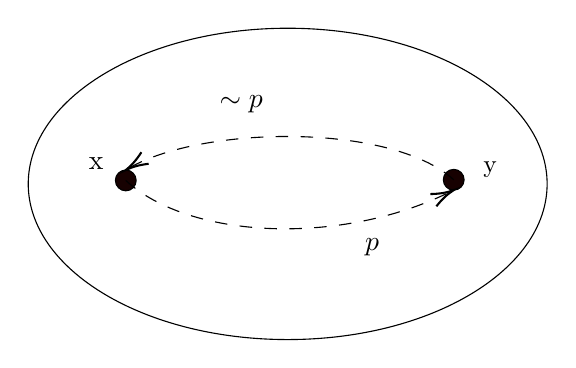
\begin{tikzpicture}[x=0.75pt,y=0.75pt,yscale=-1,xscale=1]
%uncomment if require: \path (0,300); %set diagram left start at 0, and has height of 300

%Shape: Ellipse [id:dp7216176657267284]
\draw   (220,155) .. controls (220,113.58) and (275.96,80) .. (345,80) .. controls (414.04,80) and (470,113.58) .. (470,155) .. controls (470,196.42) and (414.04,230) .. (345,230) .. controls (275.96,230) and (220,196.42) .. (220,155) -- cycle ;
%Shape: Circle [id:dp028557385614719877]
\draw  [fill={rgb, 255:red, 23; green, 1; blue, 1 }  ,fill opacity=1 ] (262,153.33) .. controls (262,150.56) and (264.24,148.33) .. (267,148.33) .. controls (269.76,148.33) and (272,150.56) .. (272,153.33) .. controls (272,156.09) and (269.76,158.33) .. (267,158.33) .. controls (264.24,158.33) and (262,156.09) .. (262,153.33) -- cycle ;
%Shape: Circle [id:dp44344880871890213]
\draw  [fill={rgb, 255:red, 23; green, 1; blue, 1 }  ,fill opacity=1 ] (420,153) .. controls (420,150.24) and (422.24,148) .. (425,148) .. controls (427.76,148) and (430,150.24) .. (430,153) .. controls (430,155.76) and (427.76,158) .. (425,158) .. controls (422.24,158) and (420,155.76) .. (420,153) -- cycle ;
%Curve Lines [id:da7287709889449594]
\draw  [dash pattern={on 4.5pt off 4.5pt}]  (267,153.33) .. controls (297.69,181.71) and (370.52,184.94) .. (423.4,158.8) ;
\draw [shift={(425,158)}, rotate = 153.7] [color={rgb, 255:red, 0; green, 0; blue, 0 }  ][line width=0.75]    (10.93,-3.29) .. controls (6.95,-1.4) and (3.31,-0.3) .. (0,0) .. controls (3.31,0.3) and (6.95,1.4) .. (10.93,3.29)   ;
%Curve Lines [id:da6566329581802051]
\draw  [dash pattern={on 4.5pt off 4.5pt}]  (425,153) .. controls (394.47,125.42) and (303.78,126.95) .. (268.57,147.38) ;
\draw [shift={(267,148.33)}, rotate = 327.9] [color={rgb, 255:red, 0; green, 0; blue, 0 }  ][line width=0.75]    (10.93,-3.29) .. controls (6.95,-1.4) and (3.31,-0.3) .. (0,0) .. controls (3.31,0.3) and (6.95,1.4) .. (10.93,3.29)   ;

% Text Node
\draw (438,143) node [anchor=north west][inner sep=0.75pt]  [font=\small] [align=left] {y};
% Text Node
\draw (381,180) node [anchor=north west][inner sep=0.75pt]   [align=left] {$\id{p}$};
% Text Node
\draw (248,141) node [anchor=north west][inner sep=0.75pt]   [align=left] {x};
% Text Node
\draw (311,111) node [anchor=north west][inner sep=0.75pt]   [align=left] {$\sim \id{p}$};

\end{tikzpicture}

\caption{A path from x to y along with its inversion}
\end{figure}

\subsection*{Functional extensionality}\label{subsec:funext}
The notion of functional extensionality implies that pointwise-equal functions are indeed equal. By postulating the existence of the $\type{Interval}$ type along with an equality type that's based on it, functional extensionality can be derived trivially as is illustrated by the below proof.

\begin{minted}[escapeinside=||,mathescape=true]{haskell}
Eq_funExt : (f : (? |$\rightarrow$| ?)) |$\Rightarrow$| (g : (? |$\rightarrow$| ?))
            |$\Rightarrow$| (p : (x : ?) |$\rightarrow$| Eq (f x) (g x)) |$\rightarrow$| Eq f g
Eq_funExt p = Eq_eq (f := |$\lambda$| i |$\Rrightarrow$| |$\lambda$| x |$\rightarrow$|
                                   Eq_uneq (p := p x) (i := i))
\end{minted}

We note that the above proof makes use of the $\eta$-equivalence of functions,
i.e. $\lambda \id{x} \rightarrow \Funapp{\id{f}}{\id{x}} \equiv \id{f}$. Another
thing that is worth noting is that we interpret erasable functions out of $\bI$
themselves as an equality type, i.e.\ if we do without the $\id{Eq\_eq}$
constructor, and if we think of $\id{Eq\_uneq}$ as the direct application of an
expression of type $\bI$ to such a function, we obtain the following
interpretation of $\id{Eq\_funExt}$ as is the case in Cubical Agda.

\begin{minted}[escapeinside=||,mathescape=true]{agda}
funExt : |$\forall$| {A B : Type |$\ell$|} {f g: A |$\rightarrow$| B}
         |$\rightarrow$| (p : (x : A) |$\rightarrow$| f x |$\equiv$| g x)
         |$\rightarrow$| f |$\equiv$| g
funExt p i x = p x i
\end{minted}

In this case, it becomes clear that $\fn{Eq\_funExt}$ is a trivial function that
does no more than swap the order of its two arguments. This is observed in
several recent proof assistants that implement cubical type theory, such as
Cubical Agda as mentioned before, as well as coolTT and redTT.\@


%% TODO: Link to the examples chapter after showing that Quot implies funExt
Functional extensionality is an important property of the equality type, it will
especially be required in order to prove the effectiveness of quotients in
\autoref{ch:quotient-effectiveness}. However, as we shall see in ???, the
existence of quotient types itself is actually sufficient to derive functional
extensionality.

%% FIXME: Should this come before the section on funext? probably
\subsection*{Congruence of equality}
This is a another typical property of equality whose proof is significantly
simplified in a system with a cubical equality.

%% Eq_cong : (x : ?A) => (y : ?A) =>
%%           (f : ?A -> ?) -> (p : Eq x y)
%%           -> Eq (f x) (f y)
%% Eq_cong = lambda f -> lambda p ->
%%             Eq_eq (f := lambda i ≡> f (Eq_uneq (p := p) (i := i)))
\begin{minted}[escapeinside=||,mathescape=true]{haskell}
Eq_cong : (x y : ?A) |$\Rightarrow$| (f : (?A |$\rightarrow$| ?)) |$\rightarrow$| (p : Eq x y)
          |$\rightarrow$| Eq (f x) (f y)
Eq_cong f p = Eq_eq (f := |$\lambda$| i |$\Rrightarrow$| f (Eq_uneq (p := p) (i := i)))
\end{minted}


Like before, we examine the definition of the theorem in Cubical Agda for a
change of perspective. We observe that the congruence of equality merely
involves applying the function $\id{f}$ to the terms at both endpoints of the
equality.

\begin{minted}[escapeinside=||,mathescape=true]{agda}
congS : |$\forall$| {A B : Type |$\ell$|} |$\rightarrow$| (f : A |$\rightarrow$| B) (p : x |$\equiv$| y) |$\rightarrow$| f x |$\equiv$| f y
congS f p i = f (p i)
\end{minted}

By appealing to the $\eta$-equivalence of the equality type described in
\autoref{sec:identity}, we also have that $\fn{Eq\_cong id p $\equiv$ p}$ holds
definitionally.

\subsection*{Transport}
The transport operation (also known as {\id{cast}}) allows us to transport
properties that are true for some type $\id{A}$ to another type $\id{B}$ if we
have a proof that $\eqtype{\id{A}}{\id{B}}$.

%% Eq_cast : (x : ?) ≡> (y : ?) ≡> (p : Eq x y) ≡> (f : ? -> ?)
%%             ≡> f x -> f y
%% Eq_cast = lambda _ ≡> lambda _ ≡> %% Two level variables
%%            lambda A ≡> %% Type of x and y
%%            lambda x ≡> lambda y ≡>
%%            lambda p ≡> lambda f ≡>
%%              lambda fx ->
%%                 I_transp (A := lambda i ≡> f (Heq_uneq
%%                                               (t := lambda _ ≡> A)
%%                                               (p := p) (i := i)))
%%                          (r := i0) fx
%%

\begin{minted}[escapeinside=||,mathescape=true]{haskell}
Eq_cast : (x y : ?A) |$\Rrightarrow$| (p : Eq x y) |$\Rrightarrow$| (f : (? |$\rightarrow$| ?)) |$\Rrightarrow$| f x
          |$\rightarrow$| f y
Eq_cast A x y p f fx =
  I_transp (A := |$\lambda$| t |$\Rrightarrow$| f (Eq_uneq (t := t) (p := p) (i := i)))
           (r := |$\ileft$|) fx
\end{minted}

Here, we make use of the built-in function $\id{I\_transp}$ by passing it the argument $\earg{\id{r}}{\ileft}$, intending it to behave as a transport function. In other words, by passing it something of type $\Funapp{\id{f}}{\id{x}}$, it returns something of type $\Funapp{\id{f}}{\id{y}}$, which is precisely what the transport/cast function is meant to do.

The $\id{I\_transp}$ function that looks slightly strange at first sight allows us to prove a certain property of the transport operation. Transporting across a reflexive path should be equivalent to a no-op, as is illustrated in the following proof.

\begin{minted}[escapeinside=||,mathescape=true]{haskell}
Eq_cast_refl : (A : Type) |$\Rrightarrow$| (x : A)
               |$\rightarrow$| Eq (Eq_cast (p := Eq_refl (x := x))
                              (f := |$\lambda$| _ |$\rightarrow$| A) x)
                     x
Eq_cast_refl A x = Eq_eq (f := |$\lambda$| i |$\Rrightarrow$|
                            I_transp (A := |$\lambda$| _ |$\Rrightarrow$| A) (r := i) x)
\end{minted}

\subsection*{J-rule}
The sole term former of the $\kw{Eq}$ only allows the construction of reflexive equalities, at first sight this leads us to believe that not much can actually be done with the $\kw{Eq}$ type. After all, if all we had were proofs of the form $x = x$, it would be difficult to imagine achieving anything with them. The true magic of the equality type lies in it's elimination principle. Traditionally, the equality type comes with an elimination principle known as the J-rule. This was first introduced by Per Martin-Löf in \cite{martin1975intuitionistic}, although it had not been given this particular name when the rule first made its appearance. (TODO:\ Where was the name J first introduced?) Suppose that we have a type family $C$ that is parametrised by two terms $x$ and $y$ of some type $A$ as well as a proof that $x$ and $y$ are equal, i.e. of type $\Funapp{\kw{Eq}}{x}{y}$. If we have have a proof term $p$ that witnesses the equality of two arbitrary terms $a$ and $b$ of type $A$, and we wish to produce a term of type $\Funapp{C}{a}{b}{p}$, then the J-rule says that it suffices for us to provide a means of producing for all $\oftype{x}{A}$ a term of type $\Funapp{C}{x}{x}{(\Funapp{\kw{refl}}{x})}$. We now state the type of the J-rule:

\begin{minted}[escapeinside=@@,mathescape=true]{haskell}
J : (C : (x : ?A) -> (y : ?A) -> Eq x y -> Type)
    -> ((x : A) -> C x x Eq_refl)
    -> (x : A) -> (y : A) -> (p : Eq x y)
    -> C x y p;
\end{minted}

This rule is essentially saying that in order to know what to do with an equality between an arbitrary $x$ and $y$, we merely need to know how to handle the case where we are dealing a reflexivity proof. Now, given the fact that the reflexivity constructor is the only constructor of the $\kw{Eq}$ type, one might think that the above elimination principle is well justified. Recall that elimination principle of an inductively defined datatype (that satisfies the positivity check, TODO: ideally I cite something here to not have to elaborate on this) can usually be derived based on the constructors of the datatype itself. For instance, consider the below inductive definition of the Peano natural numbers.

\begin{minted}{haskell}
type Nat
    | zero
    | succ Nat
\end{minted}

The corresponding elimination principle then takes on the following logical form:

\begin{minted}[escapeinside=@@,mathescape=true]{haskell}
Nat_elim : (P : Nat @$\rightarrow$@ Type)
           @$\Rrightarrow$@ P zero @$\rightarrow$@ ((n : Nat) @$\rightarrow$@ P n @$\rightarrow$@ P (succ n))
           @$\rightarrow$@ (n : Nat) @$\rightarrow$@ P n;
\end{minted}

First, we need to define what needs to be done if the natural number we are trying to eliminate is $\id{zero}$. Next, if the natural number we want to eliminate is something of the form $\Funapp{succ}{n}$, then we can imagine making a recursive call to the eliminator to produce a result for $\Funapp{succ}{n}$ for $n$, and now we need a means of transforming a proof of $\Funapp{P}{n}$ to one of $\Funapp{P}{(\Funapp{succ}{n})}$. Indeed, the elimination principle of natural numbers is just mathematical induction. Hence, it is reasonable to say that in order to eliminate an equality proof, it suffices for us define what needs to be odne for reflexivity proofs. However, as was mentioned before, we are not able to prove that all equality proofs are in fact equal to the reflexivity proof. Regardless, attempts have been made to justify the elimination principle of the equality type, although we opt not to elaborae on this here. (TODO: consider linking something on this topic here or discuss it elsewhere on the in appendix. Also, check the alternative yoneda justification to see if its worth mentioning p216 HoTT-book)

However in Typer, the elimination rule for the $\kw{Eq}$ type is not provided in the form of the J-rule, instead we have the means of using the equality proof to perform a cast. This operation is also known commonly known as `transport'. The type of the cast function is descriptive of what it does.

It is possible to derive $\kw{Eq\_cast}$ from the J-rule. The natural question that we should now ask ourselves is whether the J-rule can be derived from $\kw{Eq\_cast}$, in other words we would like to know if the two elimination principles are equivalent. It turns out that one way of doing it hinges upon whether we are able to inhabit the following type:

\begin{minted}[escapeinside=@@,mathescape=true]{haskell}
eqUnique : (A : Type) @$\Rrightarrow$@ (a b : A) (p : Eq a b)
           @$\rightarrow$@ Eq (t := Sigma A (lambda a' -> Eq a a'))
                              (sigma A Eq_refl) (sigma b p);
\end{minted}

We provide more details of this in the appendix (TODO: actually do this).

- TODO: If want to be able to prove that J can be derived from cast, we need to
leverage the fact that $(x , refl) = (y , p)$, check notes for more details.

In Typer and in intensional type theory in general, we need to explicitly invoke a cast function of some sort, this is in contrast with extensional type theory (ETT)\cite{martin1982constructive} where equality proofs in the context are automatically used by the typechecker to carry out casts whenever necessary. This is shown by the following judgement in ETT that states that equality proofs can be converted to judgemental equalities.

\begin{prooftree*}
  \hypo{\oftype{\ctx}{t}{\Funapp{\kw{Eq}}{a}{b}}}
  \infer1{\ctx \vdash a \equiv b}
\end{prooftree*}

This is also the reason why typechecking is not decidable in ETT as the necessity to invoke the above rule is not syntax directed.

\subsection*{Transitivity}\label{subsection:eqtransitivity}
Continuing our analogy of equality proofs as paths, the transitivity property allows us to concatenate two paths. We join the right endpoint of the first path with the left endpoint of the second path, producing a new path. The proof of this theorem is as follows:

\begin{minted}[escapeinside=||,mathescape=true]{haskell}
Eq_trans : (x y z: ?t) |$\Rrightarrow$| Eq x y |$\rightarrow$| Eq y z |$\rightarrow$| Eq x z
Eq_trans x y z x=y y=z = Eq_cast (p := y=z)
                                 (f := |$\lambda$| x' |$\rightarrow$| Eq x x')
                                 x=y
\end{minted}

\begin{figure}[H]
\centering
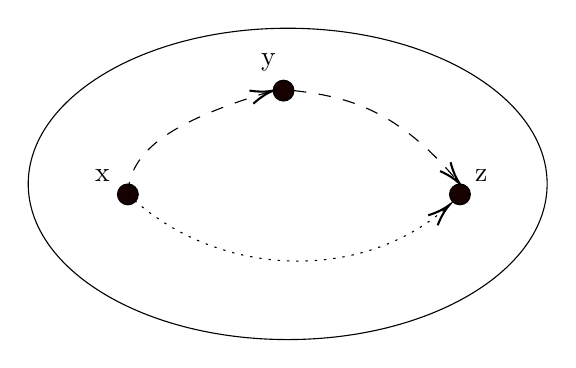
\begin{tikzpicture}[x=0.75pt,y=0.75pt,yscale=-1,xscale=1]
%uncomment if require: \path (0,300); %set diagram left start at 0, and has height of 300

%Shape: Ellipse [id:dp014634117148388581]
\draw   (210,155) .. controls (210,113.58) and (265.96,80) .. (335,80) .. controls (404.04,80) and (460,113.58) .. (460,155) .. controls (460,196.42) and (404.04,230) .. (335,230) .. controls (265.96,230) and (210,196.42) .. (210,155) -- cycle ;
%Shape: Circle [id:dp26323124675512766]
\draw  [fill={rgb, 255:red, 23; green, 1; blue, 1 }  ,fill opacity=1 ] (253,160.06) .. controls (253,157.3) and (255.24,155.06) .. (258,155.06) .. controls (260.76,155.06) and (263,157.3) .. (263,160.06) .. controls (263,162.82) and (260.76,165.06) .. (258,165.06) .. controls (255.24,165.06) and (253,162.82) .. (253,160.06) -- cycle ;
%Shape: Circle [id:dp6819431699402925]
\draw  [fill={rgb, 255:red, 23; green, 1; blue, 1 }  ,fill opacity=1 ] (328,110.06) .. controls (328,107.3) and (330.24,105.06) .. (333,105.06) .. controls (335.76,105.06) and (338,107.3) .. (338,110.06) .. controls (338,112.82) and (335.76,115.06) .. (333,115.06) .. controls (330.24,115.06) and (328,112.82) .. (328,110.06) -- cycle ;
%Curve Lines [id:da09243595336985422]
\draw  [dash pattern={on 4.5pt off 4.5pt}]  (338,110.06) .. controls (364.73,112.97) and (388.52,119.86) .. (417.13,154.01) ;
\draw [shift={(418,155.06)}, rotate = 229.87] [color={rgb, 255:red, 0; green, 0; blue, 0 }  ][line width=0.75]    (10.93,-3.29) .. controls (6.95,-1.4) and (3.31,-0.3) .. (0,0) .. controls (3.31,0.3) and (6.95,1.4) .. (10.93,3.29)   ;
%Curve Lines [id:da576198955407853]
\draw  [dash pattern={on 4.5pt off 4.5pt}]  (258,160.06) .. controls (258.99,139.27) and (277.62,125.28) .. (326.51,110.51) ;
\draw [shift={(328,110.06)}, rotate = 163.36] [color={rgb, 255:red, 0; green, 0; blue, 0 }  ][line width=0.75]    (10.93,-3.29) .. controls (6.95,-1.4) and (3.31,-0.3) .. (0,0) .. controls (3.31,0.3) and (6.95,1.4) .. (10.93,3.29)   ;
%Shape: Circle [id:dp7540304044235371]
\draw  [fill={rgb, 255:red, 23; green, 1; blue, 1 }  ,fill opacity=1 ] (413,160.06) .. controls (413,157.3) and (415.24,155.06) .. (418,155.06) .. controls (420.76,155.06) and (423,157.3) .. (423,160.06) .. controls (423,162.82) and (420.76,165.06) .. (418,165.06) .. controls (415.24,165.06) and (413,162.82) .. (413,160.06) -- cycle ;
%Curve Lines [id:da43079739398707617]
\draw  [dash pattern={on 0.84pt off 2.51pt}]  (258,160.06) .. controls (302.55,202.13) and (372.58,201.57) .. (411.82,166.14) ;
\draw [shift={(413,165.06)}, rotate = 136.9] [color={rgb, 255:red, 0; green, 0; blue, 0 }  ][line width=0.75]    (10.93,-3.29) .. controls (6.95,-1.4) and (3.31,-0.3) .. (0,0) .. controls (3.31,0.3) and (6.95,1.4) .. (10.93,3.29)   ;

% Text Node
\draw (321,91) node [anchor=north west][inner sep=0.75pt]   [align=left] {y};
% Text Node
\draw (241,147.06) node [anchor=north west][inner sep=0.75pt]   [align=left] {x};
% Text Node
\draw (424,147.06) node [anchor=north west][inner sep=0.75pt]   [align=left] {z};

\end{tikzpicture}

\caption{The concatenation of a path between x and y and a path between y and z to produce a new path between x and z.}
\end{figure}

\section{Equality as a mere proposition}
Although we say that our equality type is a proposition, it is by no means a
mere proposition (HoTT book\cite{HoTTbook} Chapter 3.3). This implies that it is
not a given that two proofs of the same equality are provably equal. In other
words, when we ask ourselves the question ``Is it the case that a = b'', we do
not only care if the answer is yes or no, if they are indeed equal, we can
interest ourselves in what ways exactly are they equal. This is in contrast to
other systems where the uniqueness of identity types (UIP) applies to all types.
Notably, this is true of systems that admit axiom
K\cite{streicher1993investigations} that states all identity proofs are equal to
the reflexivity proof, and by extension all proofs of the same equality are
equal. In the remainder of this section, we show that UIP is a property that is
true for a certain class of types in Typer.

\subsection{Hedberg's theorem}\label{subsec:hedberg}

To set the stage, we provide a few definitions. A type is said to be
\textbf{decidable} if we are able to decide whether the type is inhabited or
not. In the case where it is inhabited, we must also have a witness of such an
inhabitant. In Typer, decidability can be represented by the following inductive
type.

\begin{minted}[escapeinside=@@,mathescape=true]{haskell}
type Dec (A : Type)
  | yes A
  | no (A -> False)
\end{minted}

A type is said to be \textbf{collapsed} if any two inhabitants of the type may
be proved to be equal, this corresponds directly the notion of a mere
proposition. The two definitions that we just stated may also be used in the
context of identity types. If we have say that a type has decidable equality,
this implies that for any two terms of this type, we can decide whether or not
they are equal. On top of that, if the type has collapsed identity types, then
for any pair of terms of this type, any two proofs that they are equal are also
equal. The notion of collapsible identity types corresponds to the notion of a
$\kw{Set}$ or h-set in HoTT.

\begin{theo}[Hedberg's theorem\cite{hedberg1998coherence}]
If a type \fn{A} has decidable equality, then \fn{A} has collapsed identity
types.
\end{theo}

In this work, we provide a proof of this theorem in the form of Typer code. We
present the type of the function without going into the details of its
implementation\footnote{The actual implementation may be found in the attached \fn{samples/hedberg.typer} file}.

\begin{minted}[escapeinside=@@,mathescape=true]{haskell}
dici : (di : (x : ?A) @$\rightarrow$@ (y : ?A) @$\rightarrow$@ Dec (x @$\equiv$@ y))
       @$\rightarrow$@ (a : ?A) @$\rightarrow$@ (b : ?A)
       @$\rightarrow$@ (u : a @$\equiv$@ b) @$\rightarrow$@ (v : a @$\equiv$@ b)
       @$\rightarrow$@ u @$\equiv$@ v
\end{minted}

\section{Limitations}
We don't have primitives such as $hcomp$, what does this imply? Is there a
certain class of proofs we are unable to construct? Or do we just suffer from
some amount of inconvenience?


\chapter{Quotient Type}
\section{Typing rules}
We present the $\id{Quotient}$ primitives along with their typing rules.

\begin{prooftree*}
   \hypo{\oftype{\ctx}{\id{A}}{\kw{Type}}}
   \hypo{\oftype{\ctx}{\id{R}}{\id{A} \rightarrow \id{A} \rightarrow \kw{Type}}}
   \infer2[\kw{QUOT-FORMATION}]{\oftype{\ctx}{\Funapp{\kw{Quotient}}{\id{A}}{\id{R}}}
                                             {\kw{Type}}}
\end{prooftree*}

We introduce the $\kw{Quotient}$ type former, which takes a base type $\id{A}$
along with a relation $\id{R}$ as arguments. At this stage, we do not require
the relation to be an equivalence relation, though in order to define a
meaningful quotient type, the above requirement is often necessary. We also do
not enforce that the relation be a mere proposition, however as we will see in
\autoref{ch:quotient-effectiveness}, this is required in order for the quotient to be effective. (TODO: maybe link to more specific section instead of the chapter in general)

\begin{prooftree*}
   \hypo{\oftype{\ctx}{\id{a}}{\id{A}}}
   \hypo{\oftype{\ctx}{\Funapp{\id{Quotient}}{\id{A}}{\id{R}}}
                      {\kw{Type}}}
   \infer2[\kw{QUOT-INTRO-IN}]{\oftype{\ctx}{\Funapp{\id{Quotient\_in}}{\id{A}}{\id{R}}{\id{a}}}
                                         {\Funapp{\id{Quotient}}{\id{A}}{\id{R}}}}
\end{prooftree*}

$\id{Quotient\_in}$ is none other than a term former that injects a term of type
$\id{A}$ into a quotient under some relation.

\begin{prooftree*}
   \hypo{\oftype{\ctx}{\id{a}_1}{\id{A}}}
   \hypo{\oftype{\ctx}{\id{a}_2}{\id{A}}}
   \hypo{\oftype{\ctx}{\id{r}}{\Funapp{\id{R}}{\id{a}_1}}{\id{a}_2}}
   \infer3[\kw{QUOT-INTRO-EQ}]{
\oftype{\ctx}{\Funapp{\id{Quotient\_eq}}{\id{A}}{\id{R}}
                                        {\id{a}_1}{\id{a}_2}{\id{r}}}
             {\Funapp{\id{Quotient\_in}}{\id{A}}{\id{R}}{\id{a}_1} \equiv \Funapp{\id{Quotient\_in}}{\id{A}}{\id{R}}{\id{a}_2}}}

\end{prooftree*}

By definition, given that two terms $\id{a}_1$ and $\id{a}_2$ of type $\id{A}$
are related by some relation, then the injections of these two terms into a
quotient under the aforementioned relation should be equal. $\id{Quotient\_eq}$
is a witness of the above property.

\begin{prooftree*}
   \hypo{\oftype{\ctx}{\id{P}}{\Funapp{\id{Quotient}}{\id{A}}{\id{R}} \rightarrow \kw{Type}}}
   \hypo{\oftype{\ctx}{\id{q}}{\Funapp{\id{Quotient}}{\id{A}}{\id{R}}}}
   \infer[no rule]2{\oftype{\ctx}{\id{f}}
                           {(\oftype{\id{a}}{\id{A}}) \rightarrow \Funapp{\id{P}}{(\Funapp{\id{Quotient\_in}}{\id{A}}{\id{R}}{\id{a}})}}}
   \infer[no rule]1{\oftype{\ctx}{\id{h}}{(\oftype{\id{a}_1 \ \id{a}_2}{\id{A}})
                                          \rightarrow \Funapp{\id{R}}{\id{a}_1}{\id{a}_2}}
                                          \rightarrow \Funapp{\id{Heq}}{(\Funapp{\id{f}}{\id{a}_1})}
                                                                       {(\Funapp{\id{f}}{\id{a}_2})}}
   \infer1[\kw{QUOT-ELIM}]{\oftype{\ctx}{\Funapp{\id{Quotient\_elim}}{\id{A}}{\id{R}}{\id{f}}{\id{h}}{\id{q}}}
                                        {\Funapp{\id{P}}{\id{q}}}}
\end{prooftree*}

We would like to enable the dependent elimination of quotients, in other words
we would like to be able to eliminate a term of some quotient type
$\Funapp{\id{Quotient}}{\id{A}}{\id{R}}$ to some type family $\id{P}$ that is
indexed by the quotient type itself. To that end, we require some function
$\id{f}$ that takes some $\id{a}$ of the base type $\id{A}$ to
$\Funapp{\id{P}}{(\Funapp{\id{Quotient\_in}}{\id{A}}{\id{R}}{\id{a}})}$. In a
way, this implies that the function $\id{f}$ has the chance of `looking inside'
the quotient, and thus we also require a proof that such a function $\id{f}$
behaves consistently when applied to terms that are related by the underlying
relation of the quotient. The usage of heterogenous equality here is necessary
as $\Funapp{\id{f}}{\id{a}_1}$ and $\Funapp{\id{f}}{\id{a}_2}$ are not of the
same type. We note as well that our dependent elimination of quotients is not
limited to motives that are \type{Props}, as opposed to when quotient types are
added to a theory interpreted in a setoid model as proposed by
Li\cite{li2015quotient}.

\section{Reduction rules}
We present the computation rule for the elimination of quotients.

\begin{prooftree*}
   \hypo{\id{q} \rightsquigarrow \Funapp{\id{Quotient\_in}}{\id{A}}{\id{R}}{\id{a}}}
   \infer1[]{\Funapp{\id{Quotient\_elim}}{\id{A}}{\id{R}}{\id{f}}{\id{h}}{\id{q}}
             \rightsquigarrow \Funapp{\id{f}}{\id{a}}}
\end{prooftree*}

We note that during $\id{Quotient}$ elimination, the proof that the eliminator
function respects the $\id{Quotient}$ is ignored. Instead, the function is
applied directly to the underlying element of the base type. The fact that the
proof that the elimination respects the quotient is unused during computation
and is merely utilised during type-checking justifies our subsequent choice of
making the proof an erasable argument of $\id{Quotient\_elim}$.

It is also interesting to note that we are not able to derive a meaningful
$\eta$-rule. If we wish to apply $\id{Quotient\_in}$ after applying
$\id{Quotient\_elim}$ such that the composition amounts to the identity
function, this would imply that $\id{Quotient\_elim}$ would need to called with
a function $\id{f}$ that is itself the identity function. Unfortunately, in the
general case this would not respect the underlying relation of the quotient.
However, we could define an $\eta$-rule of sorts for quotients based on
normalisation. (TODO: discuss and link)

\section{Implementation}

In this section, we describe how the rules described above were added to Typer.
Subsequently, we describe the library that we provide to facilitate the usage of
quotient types in the development of Typer programs and proofs.

\subsection{Axioms}

Quotient types are introduced in Typer in axiomatic manner, i.e.\ the existence
of the type former, terms formers and eliminators are simply postulated.
However, the appropriate computational behaviour of the above constructs are
also added to the system whenever necessary such that we do not find ourselves
with stuck terms that adversely affect the computational properties of our
system.

\subsubsection*{Formation}
The existence of the $\id{Quotient}$ type is postulated as follows:

\begin{minted}[escapeinside=||,mathescape=true]{haskell}
Quotient : (A : Type) |$\rightarrow$| (R : A |$\rightarrow$| A |$\rightarrow$| Type) |$\rightarrow$| Type
\end{minted}

\subsubsection*{Introduction}
Two axioms are added, corresponding to the two introduction rules of $\id{Quotient}$.

\begin{minted}[escapeinside=||,mathescape=true]{haskell}
Quotient_in : (A : Type) |$\Rrightarrow$| (R : A |$\rightarrow$| A |$\rightarrow$| Type) |$\Rrightarrow$| A |$\rightarrow$| Quotient A R
Quotient_eq : (A : Type) |$\Rrightarrow$| (R A |$\rightarrow$| A |$\rightarrow$| Type)  |$\Rrightarrow$| (a a' : A) |$\Rrightarrow$| R a a'
              |$\rightarrow$| Eq (Quotient_in (R := R) a) (Quotient_in (R := R) a')
\end{minted}

TODO: In Quotient\_eq, debate the choice of not making R a a' erasable? I'm
unsure if there are any benefits of having it as non-erasable

As a constructor of equalities, $\id{Quotient\_eq}$ does not take part in
computations. As such, no special reduction rules needed to be added for it.

\subsubsection*{Elimination}

\begin{minted}[escapeinside=||,mathescape=true]{haskell}
Quotient_elim : (A : Type) |$\Rrightarrow$| (R : A |$\rightarrow$| A |$\rightarrow$| Type) |$\Rrightarrow$| (P : Quotient A R |$\rightarrow$| Type)
                |$\Rrightarrow$| ((a : A) |$\rightarrow$| P (Quotient_in a))
                |$\rightarrow$| ((a a' : A) |$\rightarrow$| R a a' |$\rightarrow$| Heq (f a) (f a')
                |$\Rrightarrow$| (q : Quotient A R) |$\rightarrow$| P q
\end{minted}

As mentioned in the previous section, the appropriate $\beta$-reduction rule is
added for the eliminator. When $\id{Quotient\_elim}$ is passed a term of the
form $\Funapp{\id{Quotient\_in}}{\id{a}}$, the entire $\id{Quotient\_elim}$ term
reduces to just $\Funapp{\id{f}}{\id{a}}$, ignoring the coherence proof that is
passed to the function as it acts simply as a form of static information.

\subsection{Syntaxique sugar}
TODO: Add more details after things get figured out

TODO: Maybe mention experience of trying to encode QITs using syntaxic sugar,
though unfortunately it didn't work out very well

\chapter{Quotient Effectiveness}\label{ch:quotient-effectiveness}

This only works for relations that are propositions and equivalence relations
(i.e.\ reflexive, symmetric and transitive).

\section{Propositional Extensionality}
We provide a alternative version of propositional extensionality that is
slightly weaker. Consequently, the version of quotient effectiveness that we
prove is also weaker.

\subsection*{Representation of propositions}

Intuitively speaking, propositions are a type that contain no intrinsic data, it
is their mere existence that counts. This is precisely the notion of proof
irrelevance. In Typer, this notion is represented via erasability. We introduce
a built-in data type that captures this idea.

\begin{minted}{haskell}
type Erased (T : Type)
  | erased (t ::: T)
\end{minted}

By ensuring that the witness $\id{t}$ of the type $\id{T}$ is erasable, this
provides us with a guarantee that during elimination, the witness $\id{t}$ can
only be used in an erasable, i.e.\ proof irrelevant manner.

To convince ourselves that this type does indeed capture the essence of a
proposition, we provide a proof of
$\Funapp{\id{isProp}}{(\Funapp{\id{Erased}}{?\id{T}})}$. We first state the
definition of $\id{isProp}$:

\begin{minted}[escapeinside=||,mathescape=true]{haskell}
isProp : (T : Type) |$\rightarrow$| Type
isProp T = (x y : T) |$\rightarrow$| Eq x y
\end{minted}

We now the present the proof in the form of Typer code.

\begin{minted}[escapeinside=@@,mathescape=true]{haskell}
erasedIsProp : (T : Type) @$\Rrightarrow$@ isProp (Erased T)
erasedIsProp t1 t2 =
  case t1
    | erased (_ := e1) @$\Rightarrow$@
        let
          p1 = ##DeBruijn 0 : Eq (erased (t := e1)) t1
        in
          case t2
            | erased (_ := e2) @$\Rightarrow$@
                let
                  p2 = ##DeBruijn 0 : Eq (erased (t := e2)) t2
                in
                  Eq_trans (Eq_comm p1) p2
\end{minted}

Typer does not offer the direct specialisation of $\kw{case}$ targets in
branches. In other words, in the first case branch, we do not have a
definitional equality between $\id{t1}$ and
$\Funapp{\id{erased}}{(\earg{\_}{\id{e1}})}$. Instead, an equality proof between
them is injected into the context, which can be accessed as the variable at
deBruijn index 0. Now that we have the two equality proofs, in order to
concatenate them\footnote{By considering equalities as path, the application of
the transitivity property of equality is conceptually similar to concatenating
two paths.}, we require $\Funapp{\id{erased}}{(\earg{\_}{\id{e1}})}$ and
$\Funapp{\id{erased}}{(\earg{\_}{\id{e2}})}$ to be equal. A priori, the two
terms are not equal as $\id{e1}$ and $\id{e2}$ are completely arbitrary.
However, Typer ignores erasable terms when checking the convertibility of terms,
this is a property that was proven to be sound in \cite{barras2008implicit} as
convertibility is tested on extracted terms. This allows the concatenation to
succeed and thus concludes the proof.

\subsection*{Implementation details}

Propositional extensionality essentially means that if two propositions that are
logically equivalent, i.e.\ each proposition implies the other, then we can say
that they are equal. And precisely because we are postulating a new equality
constructor, we have to be very careful that the resulting equality proof is
indeed proof irrelevant. In other words, we need this equality proof to not have
any runtime relevance. This is principally because we insist that the transport
operation to be a no-op during runtime. This is the motivation behind our choice
to use the $\id{Erased}$ type to represent propositions, as it is a guarantee
that such a type carries no useful runtime information. This implies that a
transport operation from one $\id{Erased}$ type to another is necessarily simply
a no-op.

In a setting with univalence, propositional extensionality is simply a theorem
that may be proven, more specifically, it may be seen as a degenerate case of univalence\cite{sozeau2013univalence}. This is a result that is
immediate as an equivalence between logically equivalent propositions is
trivial. In the setting of Typer however, propositional extensionality is
implemented as an axiom with the following type signature:

\begin{minted}[escapeinside=@@,mathescape=true]{haskell}
propExt : (A : Type) @$\Rrightarrow$@ (B : Type) @$\Rrightarrow$@ (Erased A @$\rightarrow$@ Erased B)
           @$\rightarrow$@ (Erased B @$\rightarrow$@ Erased A) @$\rightarrow$@ Erased A \equiv Erased B
\end{minted}

The above is a weaker notion of propositional extensionality compared to what is
proposed in Cubical Agda, which has the following type signature:

\begin{minted}[escapeinside=@@,mathescape=true]{Agda}
propExt : {A B : Type} @$\rightarrow$@ isProp A @$\rightarrow$@ isProp B @$\rightarrow$@ (A @$\rightarrow$@ B)
          @$\rightarrow$@ (B @$\rightarrow$@ A) @$\rightarrow$@ A @$\equiv$@ B
\end{minted}

However, this produces an equality proof that is not proof irrelevant, as
$\id{A}$ and $\id{B}$ are not necessarily the `same' type. We illustrate the
above with a simple example. We define two instances of the unit type which are
trivially `logically equivalent'.

\begin{minted}[escapeinside=@@,mathescape=true]{Agda}
data Unit1 : Type where unit1 : Unit1

data Unit2 : Type where
  unit2 : Unit2
\end{minted}

$\Funapp{\kw{isProp}}{\id{Unit1}}$ and $\Funapp{\kw{isProp}}{\id{Unit2}}$ are
trivially true, as is the case for all $\mathbb{1}$-types. $\id{Unit1}
\rightarrow \id{Unit2}$ and $\id{Unit2} \rightarrow \id{Unit1}$ are also
inhabited. Propositional extensionality thus gives us a proof of $\id{Unit1}
\equiv \id{Unit2}$. This implies that we should be able to use said proof to
transport $\id{unit1}$ to $\id{unit2}$, but since the two terms do not have the
same runtime representation, this simply cannot be a no-op. This is in stark
contrast to the version of propositional extensional that we are proposing in
Typer that only accepts types that are boxed in the $\id{Erased}$ type. We would
have no qualms about having a proof of equality between
$\Funapp{\id{Erased}}{Unit1}$ and $\Funapp{\id{Erased}}{Unit2}$ as terms of
these two types would essentially have the same runtime representation. It is
also for this precise reason that our version of propositional extensionality is
weaker, as we are constrained to construct an equality proof that is not
computationally relevant.

Another worthy comparison to make is with Lean, which has a $\kw{Prop}$ sort.
Terms of this sort are not autorised to be used in a proof relevant manner. Its
version of propositional extensionality has the following form:

\begin{minted}[escapeinside=@@,mathescape=true]{lean}
axiom propext {a b : Prop} : (a @$\leftrightarrow$@ b) @$\rightarrow$@ a = b
\end{minted}

This is similar to what we have in Typer, except that proof irrelevance is
enforced in a different manner.

\section{Equivalence relation}

First, we state what we mean when we say `relation' to set the stage for the
subsequent discussion. For our purposes, we consider binary relations, which are
type formers that take two arguments of some type $\kw{A}$. Assuming that we
call the relation $\kw{R}$ and its two arguments $\id{a}$ and $\id{a}'$
respectively, inhabitants of the type $\Funapp{\kw{R}}{\id{a}}{\id{a}'}$ are
witnesses of this binary relation. The type signature of a binary relation has
the below form:

\begin{minted}[escapeinside=||,mathescape=true]{haskell}
R : (A : Type) |$\Rrightarrow$| (a : A) |$\rightarrow$| (a' : A) |$\rightarrow$| Type
\end{minted}

For a quotient to be effective, its underlying relation has to be an equivalence relation, we shall use this property in the proof in the subsequent section. Recall that an equivalence relation implies that the relation is reflexive, symmetric and transitive. For it to be reflexive, it needs to be the case that given an arbitrary $\oftype{\id{a}}{\kw{A}}$, $\Funapp{\kw{R}}{\id{a}}{\id{a}}$ must be trivially inhabited. The symmetry of the relation implies that if we are given an arbitrary witness of $\Funapp{\kw{R}}{\id{a}}{\id{a}'}$, we need to be able to transform that into an inhabitant of $\Funapp{\kw{R}}{\id{a}'}{\id{a}}$. The relation is transitive if we are able to transform witnesses of $\Funapp{\kw{R}}{\id{a}}{\id{b}}$ and $\Funapp{\kw{R}}{\id{b}}{\id{c}}$ into witnesses of $\Funapp{\kw{R}}{\id{a}}{\id{c}}$\footnote{The equality type fulfills these criteria and is an equivalence relation.}.

In the built-in library, we define the following type as a witness that a certain relation is indeed an equivalence relation.

\begin{minted}{haskell}
type isEquivRel (A : Type) (R : A -> A -> Type) : Type
  | equivRel (isRefl : (a : A) -> R a a)
             (isSym : (a : A) -> (b : A) -> R a b -> R b a)
             (isTrans : (a : A) -> (b : A) -> (c : A)
                         -> R a b -> R b c -> R a c)
\end{minted}

\section{Proof}
Given two arbitrary elements $\id{a}$ and $\id{a}'$ of a base type $\kw{A}$, a quotient is said to be effective if given a proof that the injection of $\id{a}$ and $\id{a}'$ into the quotient are equal, then it must be the case that $\Funapp{\kw{R}}{\id{a}}{\id{a}'}$ is true, i.e.\ we are able to find an inhabitant of it. A sufficient condition for a quotient to be effective is that the underlying relation must be both a proposition and an equivalence relation.


For an arbitrary binary relation $\kw{R}$, we can define the following:

\begin{minted}[escapeinside=||,mathescape=true]{haskell}
ErasedR : (A : Type) |$\Rrightarrow$| (A |$\rightarrow$| A |$\rightarrow$| Type) |$\rightarrow$| A |$\rightarrow$| A |$\rightarrow$| Type
ErasedR R a b = Erased (R a b)
\end{minted}

Now, we state the proof of the effectiveness of quotients in the form of Typer code

\begin{minted}[escapeinside=||,mathescape=true]{haskell}
effective : (A : Type) |$\Rrightarrow$| (R : A |$\rightarrow$| A |$\rightarrow$| Type)
            |$\rightarrow$| isEquivRel A (ErasedR R) |$\rightarrow$| (a : A) |$\rightarrow$| (b : A)
            |$\rightarrow$| Eq (Quotient_in (R := ErasedR R) a)
                  (Quotient_in (R := ErasedR R) b)
            |$\rightarrow$| ErasedR R a b
effective = lambda A |$\Rrightarrow$| lambda R equiv a b eq |$\rightarrow$|
  let
    helper : Quotient A (ErasedR R) -> Type
    helper x =
      Quotient_rec
        (R := ErasedR R)
        (lambda c |$\rightarrow$| ErasedR R a c)
        (p := lambda c d cd |$\rightarrow$|
          let
            ac->ad : Erased (R a c) |$\rightarrow$| Erased (R a d)
            ac->ad ac = equiv.isTrans a c d ac cd
            ad->ac : Erased (R a d) |$\rightarrow$| Erased (R a c)
            ad->ac ad = equiv.isTrans a d c ad
                                      (equiv.isSym c d cd)
          in
            propExt ac->ad ad->ac)
        x
    aa=ab : Eq (Erased (R a a)) (Erased (R a b))
    aa=ab = Eq_cong helper eq
  in
    Eq_cast (p := aa=ab) (f := id) (equiv.isRefl a)
\end{minted}

Compared to the more general version of the theorem we state before, here we insist that the quotient we consider be based on the erased version of some binary relation $\kw{R}$. And instead of proving that the base relation itself holds for some $\id{a}$ and $\id{b}$, we can only show that the erased version of this relation holds.

In this proof, we can see that all aspects of the sufficient condition are at
play. It is mainly used to prove that for arbitrary terms $\id{a}$, $\id{b}$ and
$\id{c}$ of type $\kw{A}$, if it is the case that if
$\Funapp{\id{Erased}}{(\Funapp{\kw{R}}{\id{b}}{\id{c}})}$ is inhabited, then
$\Funapp{\id{Erased}}{(\Funapp{\kw{R}}{\id{a}}{\id{b}})}$ $\iff$
$\Funapp{\id{Erased}}{(\Funapp{\kw{R}}{\id{a}}{\id{c}})}$. Intuitively speaking
this makes a lot of sense,
$\Funapp{\id{Erased}}{(\Funapp{\kw{R}}{\id{b}}{\id{c}})}$ implies that $\id{b}$
and $\id{c}$ are in the same equivalence class of the quotient. Hence, if we
know that $\id{a}$ is in the same equivalence class as $\id{b}$, we should
naturally be able to infer that $\id{a}$ and $\id{c}$ are also in the same
equivalence class, and vice versa. Propositional extensionality takes us even
further, by allowing us to prove that
$\Funapp{\id{Erased}}{(\Funapp{\kw{R}}{\id{a}}{\id{b}})}$ and
$\Funapp{\id{Erased}}{(\Funapp{\kw{R}}{\id{a}}{\id{c}})}$ are equal since they
are both mere propositions.

Examples of usage of the above theorem are in Chapter XXX (TODO: Link to other section).

\chapter{Examples}
The addition of quotient types to Typer allows us to define certain constructs
that are typically defined in set theory as quotient sets. In this chapter, we
discuss some types that are now natively definable by taking the quotient of
existing types in the system.

\section{Rational numbers}
To define the rational numbers as a quotient type, we have two obvious options for the base type.

The first option is as follows:

\begin{align*}
  & \mathbb{Q} \ \coloneqq \mathbb{Z} \times \mathbb{N} / \sim_{\mathbb{Q}} \\
  & (z_1 , n_1) \sim_{\mathbb{Q}} (z_2 , n_2) \ \coloneqq Eq \ (z_1 * (n_2 + 1)) \ (z_2 * (n_1 + 1))
\end{align*}

A pair $(z , n)$ represents the rational number $z / (n + 1)$, this trick allows us to ensure that the denominator is non-zero.

The second option is similar to the first:

\begin{align*}
  & \mathbb{Q} \ \coloneqq \Sigma_{\oftype{(x, y)}{\mathbb{Z} \times \mathbb{Z}}} . y \ne 0 / \sim_{\mathbb{Q}} \\
  & (x_1 , y_1, \_) \sim_{\mathbb{Q}} (x_2 , y_2, \_) \ \coloneqq Eq \ (x_1 * y_2) \ (y_1 * x_2)
\end{align*}

In this definition, the base type of a quotient is a pair of integers, along
with a proof that the denominator is non-zero. We chose to use this as the basis
of our definition of the rationals, as it is more convenient to work with a pair
of elements of the same type.

Given that the equivalence of rational numbers is captured by a relation, we do
not need to normalise our rational numbers before or after each computation,
instead we prove that all of our operations respect the equivalence of rational
numbers. We hoped that this would give us better runtime efficiency, as opposed
to more naives implementations. To make this clearer, we illustrate one possible
naive implementation. To ensure that operations on the base type of the quotient
type that we intend to use to represent the rational numbers respect the
equivalence relation, we may be tempted to simply normalise the operands before
actually carrying out any computation. This implies that if the operands were
indeed equivalent, then the normalisation of the operands would have yielded two
terms that are provably equal. Hence by the congruence property of equality, the
operation would necessarily respect the underlying relation. However, it is
clear that such an approach might possibly be expensive. In order to normalise
the base type, which we could imagine to be a pair of integers, we would have to
divide both integers by their greatest commmon divisor (GCD). The calculation of
their GCD could in itself be more costly that the actual operation itself. Thus,
this unnecessary normalisation could potentially adversely affect the runtime
efficiency of our operations on rational numbers. Hence, our definitions of
operations on the rational numbers do not rely on normalisation. However, this
is not without its downsides as it entails heavier proof obligations, this is a
topic that we shall discuss subsequently.

Typer has a built-in $\kw{Integer}$ type. Behind the scenes, this is based on
big integers in OCaml (TODO:\ Maybe some more elaboration here). Operations on
the typer $\kw{Integer}$ type such as addition, multiplication etc are
implemented as axioms. At runtime, the responsibilities of these functions are
simply delegated to their corresponding OCaml functions to carry out the
necessary computations. So far, we are unable to reason about these operations
in Typer as they are merely primitives that are implemented in the host
language. In the following section, we propose the addition of several axioms
that serve as witnesses of certain properties of the built-in $\kw{Integer}$
type, this will be crucial when we start reasoning about operations on rational
numbers.

\subsection*{Integer axioms}
We start off by axiomatising the associativity and commutativity of the addition and multiplication operations.

\begin{minted}[escapeinside=||,mathescape=true]{haskell}
Integer_+-comm : (x : Integer) |$\rightarrow$| (y : Integer)
                 |$\rightarrow$| Eq (Integer_+ x y) (Integer_+ y x)

Integer_+-assoc : (x : Integer) |$\rightarrow$| (y : Integer) |$\rightarrow$| (z : Integer)
                  |$\rightarrow$| Eq (Integer_+ x (Integer_+ y z))
                        (Integer_+ (Integer_+ x y) z)

Integer_*-comm : (x : Integer) |$\rightarrow$| (y : Integer)
                 |$\rightarrow$| Eq (Integer_* x y) (Integer_* y x)

Integer_*-assoc : (x : Integer) |$\rightarrow$| (y : Integer) |$\rightarrow$| (z : Integer)
                  |$\rightarrow$| Eq (Integer_* x (Integer_* y z))
                        (Integer_* (Integer_* x y) z)
\end{minted}

We also want to be able to show that multipication is distributive with respect to addition. We only add left distributivity as an axiom, as right distributivity can be easily proven as a theorem, this is also the case for the other axioms that we will describe below.

\begin{minted}[escapeinside=||,mathescape=true]{haskell}
Integer_*DistL+ : (x : Integer) |$\rightarrow$| (y : Integer) |$\rightarrow$| (z : Integer)
                  |$\rightarrow$| Eq (Integer_* (Integer_+ x y) z)
                        (Integer_+ (Integer_* x z) (Integer_* y z))
\end{minted}

The above properties can also be stated for the subtraction operation. We also want to be able to say that we have additive inverses for all integers and that 0 is the additive identity.

\begin{minted}[escapeinside=||,mathescape=true]{haskell}
Integer_+Linv : (x : Integer) |$\rightarrow$| Eq (Integer_+ (Integer_- 0 x) x) 0

Integer_+Lid : (x : Integer) |$\rightarrow$| Eq (Integer_+ 0 x) x
\end{minted}

Of course, we should also be able to say that 1 is the multiplicative identity.

\begin{minted}[escapeinside=||,mathescape=true]{haskell}
Integer_*Lid : (x : Integer) |$\rightarrow$| Eq (Integer_* 1 x) x
\end{minted}

Now that we have all these axioms, we can say that $\kw{Integer}$ fulfills the properties of a commutative ring. Aside from these axioms, there are some other properties that we require in order to be able to construct some useful operations on the resulting $\kw{Rational}$ type. Notably, we need to be able to say that if the product of two integers is zero, then at least one of them is zero. We formulate this in the following manner:

\begin{minted}[escapeinside=||,mathescape=true]{haskell}
Integer_isIntegral : (x : Integer) |$\rightarrow$| (y : Integer)
                     |$\rightarrow$| Eq (Integer_* x y) 0 |$\rightarrow$| (Eq x 0 |$\rightarrow$| Void)
                     |$\rightarrow$| Eq y 0
\end{minted}

Here, $\kw{Void}$ is the $\mathbb{0}$ type (also known as the empty type or bottom). This axiom essentially states that if a product $x \cdot y = 0$, then $x \ne 0 \rightarrow y = 0$.

Another useful axiom to have is one that asserts that 0 is an absorbing element with respect to multiplication. In other words, multiplying by 0 always yields 0 as a result.

\begin{minted}[escapeinside=||,mathescape=true]{haskell}
Integer_*Lzero : (x : Integer) |$\rightarrow$| Eq (Integer_* 0 x) 0
\end{minted}

\subsection*{Integer theorems}\label{subsection:int-theorems}
As stated in the subsequent section, we only added the `left' version of some axioms, as their `right' counterparts may be trivially proven as theorems based on the commutativity property of addition and multiplication.

\begin{minted}[escapeinside=||,mathescape=true]{haskell}
Integer_+Rid : (x : Integer) |$\rightarrow$| Eq (Integer_+ x 0) x
Integer_+Rid x = Eq_trans (Integer_+-comm x 0) (Integer_+Lid x)

Integer_+Rinv : (x : Integer) |$\rightarrow$| Eq (Integer_+ x (Integer_- 0 x)) 0
Integer_+Rinv x = Eq_trans (Integer_+-comm x (Integer_- 0 x))
                           (Integer_+Linv x)

Integer_*Rid : (x : Integer) |$\rightarrow$| Eq (Integer_* x 1) x
Integer_*Rid x = Eq_trans (Integer_*-comm x 1) (Integer_*Lid x)

Integer_*Rzero : (x : Integer) |$\rightarrow$| Eq (Integer_* x 0) 0
Integer_*Rzero x = Eq_trans (Integer_*-comm x 0) (Integer_*Lzero x)

Integer_*DistR+ : (x : Integer) |$\rightarrow$| (y : Integer) |$\rightarrow$| (z : Integer)
                  |$\rightarrow$| Eq (Integer_* x (Integer_+ y z))
                        (Integer_+ (Integer_* x y) (Integer_* x z))
Integer_*DistR+ x y z =
  Eq_trans (Integer_*-comm x (Integer_+ y z))
           (Eq_trans (Integer_*DistL+ y z x)
                     (Eq_trans (Eq_cong (lambda e |$\rightarrow$|
                                           Integer_+ e (Integer_* z x))
                                        (Integer_*-comm y x))
                               (Eq_cong (lambda e |$\rightarrow$|
                                           Integer_+ (Integer_* x y) e)
                                        (Integer_*-comm z x))))
\end{minted}

Another useful theorem that we can prove states that the product of two non-zero integers is necessarily non-zero.

\begin{minted}[escapeinside=||,mathescape=true]{haskell}
Integer_0-product : (x : Integer) |$\rightarrow$| (y : Integer)
                    |$\rightarrow$| (Eq x 0 |$\rightarrow$| Void) |$\rightarrow$| (Eq y 0 |$\rightarrow$| Void)
                    |$\rightarrow$| (Eq (Integer_* x y) 0 |$\rightarrow$| Void)
Integer_0-product x y x|$\ne$|0 y|$\ne$|0 xy|$\ne$|0 =
    y|$\ne$|0 (Integer_isIntegral x y xy|$\ne$|0 x|$\ne$|0)
\end{minted}

We will eventually also make use of the below theorem that states that the negation of an integer may be distributed over multiplication. Its `right' counterpart may also be proven in a similar manner.

\begin{minted}[escapeinside=||,mathescape=true]{haskell}
Integer_NegateDistL* : (x : Integer) |$\rightarrow$| (y : Integer)
                        |$\rightarrow$| Eq (Integer_- 0 (Integer_* x y))
                              (Integer_* (Integer_- 0 x) y)
Integer_NegateDistL* x y =
  Integer_- 0 (Integer_* x y)
  ==< Eq_cong (lambda e |$\rightarrow$| Integer_- e (Integer_* x y))
              (Eq_comm (Integer_*Lzero y)) >==
  Integer_- (Integer_* 0 y) (Integer_* x y)
  ==< Eq_comm (Integer_*DistL- 0 x y) >==
  Integer_* (Integer_- 0 x) y |$\qed$|
\end{minted}

\subsection*{Implementation of Rationals}
As stated before, the base type of our quotient type is essentially a pair of integers along with a proof that the second integer is non-zero. We decided to implement this as an inductive type with a single constructor.

\begin{minted}[escapeinside=@@,mathescape=true]{haskell}
type @$\mathbb{Z}{\times}\mathbb{Z}{\ne}0$@
  | inR (@$z_1$@ : Integer) (@$z_2$@ : Integer) (p : Not (Eq @$z_2$@ 0))
\end{minted}

$\kw{Not}$ has the typical definition as follows:
\begin{minted}[escapeinside=@@,mathescape=true]{haskell}
Not : (T : Type) @$\rightarrow$@ Type
Not T = T @$\rightarrow$@ Void
\end{minted}

The underlying relation takes on the following form, this can be proven to be an equivalence relation.
\begin{minted}[escapeinside=@@,mathescape=true]{haskell}
equal@$\mathbb{Q}$@ : @$\zpair$@ @$\rightarrow$@ @$\zpair$@ @$\rightarrow$@ Type
equal@$\mathbb{Q}$@ p1 p2 = Eq (p1.z1 * p2.z2) (p1.z2 * p2.z1)
\end{minted}

Finally, we can state the definition of the Rationals.

\begin{minted}[escapeinside=@@,mathescape=true]{haskell}
Rational : Type
Rational = Quotient @$\zpair$@ equal@$\mathbb{Q}$@
\end{minted}

As a sanity check, we prove that the resulting $\kw{Rational}$ type is indeed a field as it should be. Negation is the simplest operation that we can define on the rationals, it is achieved by simply negating the integer numerator. This is done via the below function.

\begin{minted}[escapeinside=@@,mathescape=true]{haskell}
negate_fst : @$\zpair \rightarrow \zpair$@
negate_fst x = inR (-1 * x.z1) x.z2 x.p
\end{minted}

We also need to prove that $\id{negate\_fst}$ respects the underlying relation $equal\mathbb{Q}$. In other words, we need to prove the following:

\begin{minted}[escapeinside=@@,mathescape=true]{haskell}
negate_compat : (a : @$\zpair$@) @$\rightarrow$@ (b : @$\zpair$@) @$\rightarrow$@
                @$\equalq$@ a b @$\rightarrow$@ @$\equalq$@ (negate_fst a) (negate_fst b)
negate_compat a b r =
    (-1 * a.z1) * b.z2
    ==< Eq_comm (Integer_*-assoc -1 a.z1 b.z2) >==
    -1 * (a.z1 * b.z2)
    ==< Eq_cong (lambda e @$\rightarrow$@ -1 * e) r >==
    -1 * (a.z2 * b.z1)
    ==< Integer_*-assoc -1 a.z2 b.z1 >==
    (-1 * a.z2) * b.z1
    ==< Eq_cong (lambda e @$\rightarrow$@ e * b.z1)
                (Integer_*-comm -1 a.z2) >==
    (a.z2 * -1) * b.z1
    ==< Eq_comm (Integer_*-assoc a.z2 -1 b.z1) >==
    a.z2 * (-1 * b.z1) @$\qed$@
\end{minted}

We introduced equational reasoning to facilitate the development and reading of such proofs, more details are given in Section~\ref{section:eqreasoning} of the appendix.

Finally, the negation operation of rational numbers can be constructed like so:

\begin{minted}[escapeinside=@@,mathescape=true,samepage]{haskell}
Rational_negate : Rational @$\rightarrow$@ Rational
Rational_negate x =
  qcase (x : @$\zpair$@ / @$\equalq$@)
    | Quotient_in a @$\Rightarrow$@ Quotient_in (R := @$\equalq$@) (negate_fst a)
    | Quotient_eq a a' r @$\Rightarrow$@ Quotient_eq (R := @$\equalq$@)
                                        (a := negate_fst a)
                                        (a' := negate_fst a')
                                        (negate_compat a a' r)
\end{minted}

We can also define the addition operation on the rationals. As before, we start off by defining a function that operates on expressions of the base type.

\begin{minted}[escapeinside=@@,mathescape=true,samepage]{haskell}
@$\zpairplus$@ : @$\zpair$@ @$\rightarrow$@ @$\zpair$@ @$\rightarrow$@ @$\zpair$@
@$\zpairplus$@ a b = inR ((a.z1 * b.z2) + (b.z1 * a.z2))
                 (a.z2 * b.z2)
                 (Integer_0-product a.z2 b.z2 a.p b.p)
\end{minted}

This is an operation that can be shown to be commutative with respect to the equivalence relation.

\begin{minted}[escapeinside=@@,mathescape=true,samepage]{haskell}
@$\zpairplus$-Comm@ : (a : @$\zpair$@) @$\rightarrow$@ (b : @$\zpair$@)
               @$\rightarrow$@ Eq (t := Quotient @$\zpair$@ @$\equalq$@)
                     (Quotient_in (@$\zpairplus$@+ a b)) (Quotient_in (@$\zpairplus$@+ b a))
@$\zpairplus$-Comm@ a b =
  let
    compat =
      (a.z1 * b.z2 + b.z1 * a.z2) * (b.z2 * a.z2)
        ==< Eq_cong (lambda e @$\rightarrow$@ (a.z1 * b.z2 + b.z1 * a.z2) * e)
                    (Integer_*-comm b.z2 a.z2) >==
      (a.z1 * b.z2 + b.z1 * a.z2) * (a.z2 * b.z2)
        ==< Integer_*-comm (a.z1 * b.z2 + b.z1 * a.z2) (a.z2 * b.z2) >==
      a.z2 * b.z2 * (a.z1 * b.z2 + b.z1 * a.z2)
        ==< Eq_cong (lambda e @$\rightarrow$@ a.z2 * b.z2 * e)
                    (Integer_+-comm (a.z1 * b.z2) (b.z1 * a.z2)) >==
      a.z2 * b.z2 * (b.z1 * a.z2 + a.z1 * b.z2) @$\qed$@
  in
      Quotient_eq (R := @$\equalq$@)
                  (a  := @$\zpairplus$@+ a b)
                  (a' := @$\zpairplus$@+ b a)
                  compat
\end{minted}

We still need to show that the $\zpairplus$ function itself respects the underlying relation, and since this is a binary operation, we will have to prove it for `both sides'. In other words, we have to produce the below proofs.

\begin{minted}[escapeinside=@@,mathescape=true,samepage]{haskell}
@$\mathbb{Q}$+\_feql@ : (a : @$\zpair$@) @$\rightarrow$@ (a' : @$\zpair$@) @$\rightarrow$@ (b : @$\zpair$@) @$\rightarrow$@ @$\equalq$@ a a'
          @$\rightarrow$@ Eq (t := Quotient @$\zpair$@ @$\equalq$@)
                (Quotient_in (@$\zpairplus$@ a b))
                (Quotient_in (@$\zpairplus$@ a' b))
@$\mathbb{Q}$+\_feql@ = ?

@$\mathbb{Q}$+\_feqr@ : (a : @$\zpair$@) @$\rightarrow$@ (b : @$\zpair$@) @$\rightarrow$@ (b' : @$\zpair$@) @$\rightarrow$@ @$\equalq$@ b b'
          @$\rightarrow$@ Eq (t := Quotient @$\zpair$@ @$\equalq$@)
                (Quotient_in (@$\zpairplus$@ a b))
                (Quotient_in (@$\zpairplus$@ a b'))
@$\mathbb{Q}$+\_feqr@ = ?
\end{minted}

The proof of $\mathbb{Q}{+}\_\kw{feql}$ is long and uninteresting and thus will not described here\footnote{Interested readers may find the proof at TODO:\ link}. However, once this has been proved, its counterpart is a trivial corollary by virtue of the commutativity of $\zpairplus$.

\begin{minted}[escapeinside=@@,mathescape=true,samepage]{haskell}
@$\mathbb{Q}$+\_feqr@ a b b' p =
    Eq_trans (@$\zpairplus$-Comm@ a b)
             (Eq_trans (@$\mathbb{Q}$@+_feql b b' a p) (@$\zpairplus$-Comm@ b' a))
\end{minted}

We can now assemble the above to define both the addition and subtraction of rationals as follows:

\begin{minted}[escapeinside=@@,mathescape=true,samepage]{haskell}
Rational_+ : Rational @$\rightarrow$@ Rational @$\rightarrow$@ Rational
Rational_+ a b =
  Quotient_rec2 (R := @$\equalq$@) (S := @$\equalq$@)
                Rational_isSet (lambda x y @$\rightarrow$@ Quotient_in (@$\zpairplus$@ x y))
                @$\mathbb{Q}$+\_feql@ @$\mathbb{Q}$+\_feqr@ a b

Rational_- : Rational @$\rightarrow$@ Rational @$\rightarrow$@ Rational
Rational_- a b = Rational_+ a (Rational_negate b)
\end{minted}

$\kw{Quotient\_rec2}$ is a library function that allows us to simultaneously eliminate two quotient expressions, more details are given in Section ??? (TODO:\ Add this). Finally, we want to prove that negation of a rational produces its additive inverse. We define $\kw{Rational\_0}$ to be the additive identity using a trivial representative of its equivalence class.

\begin{minted}[escapeinside=@@,mathescape=true]{haskell}
@$\zpairplus$@-Linv : (a : @$\zpair$@) @$\rightarrow$@ Eq (t := Rational)
                              (Quotient_in (@$\zpairplus$@ (negate_a.z1) a))
                              Rational_0
@$\zpairplus$@-Linv a =
  let
    h : Eq ((-1 * a.z1 * a.z2 + a.z1 * a.z2) * 1)
           (a.z2 * a.z2 * 0)
    h =
      (-1 * a.z1 * a.z2 + a.z1 * a.z2) * 1
      ==< Eq_cong (lambda e @$\rightarrow$@ (e * a.z2 + a.z1 * a.z2) * 1)
                  (Integer_Negate@$\equiv$@ a.z1) >==
      ((0 - a.z1) * a.z2 + a.z1 * a.z2) * 1
      ==< Integer_*Rid ((0 - a.z1) * a.z2 + a.z1 * a.z2) >==
      (0 - a.z1) * a.z2 + a.z1 * a.z2
      ==< Eq_cong (lambda e @$\rightarrow$@ e + a.z1 * a.z2)
                  (Eq_comm (Integer_NegateDistL* a.z1 a.z2)) >==
      (0 - (a.z1 * a.z2)) + a.z1 * a.z2
      ==< Integer_+-comm (0 - (a.z1 * a.z2)) (a.z1 * a.z2) >==
      a.z1 * a.z2 + (0 - (a.z1 * a.z2))
      ==< Integer_+Rinv (a.z1 * a.z2) >==
      0
      ==< Eq_comm (Integer_*Rzero (a.z2 * a.z2)) >==
      a.z2 * a.z2 * 0 @$\qed$@
  in
    Quotient_eq (R := @$\equalq$@)
                (a := @$\zpairplus$@ (negate_a.z1) a)
                (a' := inR 0 1 Integer_1@$\ne$@0)
                h

Rational_+Linv : (q : Rational) @$\rightarrow$@ Eq (Rational_+ (Rational_negate q) q)
                                      Rational_0
Rational_+Linv q =
  Quotient_elimProp (R := @$\equalq$@)
                    (P := lambda q @$\rightarrow$@
                            Eq (Rational_+ (Rational_negate q) q)
                               Rational_0)
                    (lambda q @$\rightarrow$@
                        Rational_isSet (Rational_+ (Rational_negate q) q)
                                       Rational_0)
                    @$\zpairplus$@-Linv q

Rational_+Rinv : (q : Rational) @$\rightarrow$@ Eq (Rational_+ q (Rational_negate q))
                                      Rational_0
Rational_+Rinv q = Eq_trans (Rational_+-Comm q (Rational_negate q))
                            (Rational_+Linv q)

\end{minted}

For brevity, we do not describe the proofs for multiplication as they can be
carried out in a similar fashion as above.

\subsection{Benchmarks}

%% TODO: If I end up running benchmarks for other examples as well, maybe then I
%% should consider having a dedicated section for benchmarks

In this section, we use our implementation of rational numbers to explore the
runtime cost of using quotient types in Typer. Quotient types are nothing more
than a means of using the type system to ensure that programmers respect a
certain relation on a base type by means of proof obligations. Such proofs can
be expected to be erased before the actual execution of a program, our intuition
would then lead us to expect that the usage of quotient types to have a
negligible runtime overhead. Hence, the tests in our benchmark were designed
with the simple objective of verifying the above claim.

Since the operations on rational numbers are essentially wrappers around
operations on the base type $\zpair$, our benchmark simply compares the
execution time of operations on $\zpair$ with their $\fn{Rational}$
counterparts\footnote{The code for this may be found in the
$\fn{rational\_benchmark.typer}$ file.}. We examine the runtime
cost\footnote{The tests were executed on the author's 2018 Macbook Pro with a
quadcore 2.3GHz Intel Core i5 processor with 8GB of RAM.} of
$\fn{Rational\_negate}$, $\fn{Rational\_+}$, $\fn{Rational\_-}$ and
$\fn{Rational\_*}$.

%% TODO: Column sizes aren't equal between zpair and Rational? How do I fix this?
\begin{table}[H]
\centering
\begin{tabular}{ccccc}
\hline
\multirow{2}{*}{\textbf{Operation}} & \multicolumn{2}{c}{\textbf{Execution Time (seconds)}} & \multicolumn{2}{c}{\textbf{Overhead}} \\ \cline{2-5}
                                    & \textbf{$\zpair$}          & \textbf{Rational}         & \textbf{seconds}     & \textbf{\%}    \\ \hline
Negation       & 0.39 & 0.53 & 0.14 & 35.9 \\
Addition       & 0.64 & 0.87 & 0.23 & 35.9 \\
Subtraction    & 0.76 & 1.15 & 0.39 & 51.3 \\
Multiplication & 0.50 & 0.80 & 0.30 & 60.0 \\ \hline
\end{tabular}
\caption{The runtime cost of operations on rational numbers with and without the
  use of quotient types.}
\label{tab:rational-benchmark}
\end{table}

We observe that there is indeed a non-negligible overhead caused by the usage of
quotient types, which we will now try to justify. Without loss of generality, we
discuss the addition operation. Once the $\zpairplus$ function that handles the
addition of $\zpair$ and its $\fn{Rational}$ counterpart, $\fn{Rational\_+}$
have undergone erasure, the resulting functions are extensionally equal. By
definition of erasure\cite{monnier2019typer}, all erasable arguments are
removed, hence all proof objects required by the quotient type will be absent in
the erased versions of the above functions. The two erased functions are
nevertheless not completely equal, as we shall see by examining the Elexp
(erased lambda expression) \cite{delaunay2017implementation} of
$\fn{Rational\_+}$:

\begin{minted}[escapeinside=@@,mathescape=true]{scheme}
  (lambda (a) @$\rightarrow$@ (lambda (b) @$\rightarrow$@
    (Quotient_rec2 (lambda (x) @$\rightarrow$@
                       (lambda (y) @$\rightarrow$@
                           (Quotient_in (@$\zpairplus$@ x y)))) a b)))
\end{minted}

Through a series of $\eta$-reductions and $\beta$-reductions, we can see that
the above expression is equivalent to $\zpairplus$. This implies that with an
appropriate optimisation phase, Elexps containing quotient primitives could be
simplified to completely neutralise the overhead of quotient types. We leave
this optimisation for a future work.

\section{Multiset}

TODO: Cook up an example of this

\section{Propositional Truncation}

We can encode propositional truncation as a quotient type. The required properties are:

\begin{itemize}
	\item $\id{A} \ \kw{true} \rightarrow \norm{A} \ \kw{true}$ and $\norm{A}$
      is a subsingleton (exists unique)
%% 	\item $\id{A}  \ $subsingleton$ \rightarrow (\norm{A} \ \kw{true} \rightarrow \id{A} \ \kw{true})$
	\item For some P that is a subsingleton and some $f : \id{A} \rightarrow \kw{P}$, there exists a function $g : \norm{A} \rightarrow P$ s.t. $ \forall a : A \ . \ g(a^*) = f(a)$, where $a^* \in \norm{A}$.
\end{itemize}

The encoding is simple, we simply define the following type former along with its term former:

\begin{minted}[escapeinside=@@,mathescape=true]{haskell}
PropTrunc : (P : Type) @$\rightarrow$@ Type
PropTrunc P = Quotient P (@$\lambda$@ p1 p2 @$\rightarrow$@ Unit)

inPropTrunc : (P : Type) @$\Rrightarrow$@ P @$\rightarrow$@ PropTrunc P
inPropTrunc p = Quotient_in (R := @$\lambda$@ p1 p2 @$\rightarrow$@ Unit) p
\end{minted}

The choice of $\id{R}$ here essentially implies that every term of the base type $\kw{P}$ shall be equated in the resulting quotient type. This is witnessed by the following function:

\begin{minted}[escapeinside=@@,mathescape=true]{haskell}
squash : (P : Type) @$\Rrightarrow$@ (x : PropTrunc P) @$\rightarrow$@ (y : PropTrunc P) @$\rightarrow$@ Eq x y
squash = @$\lambda$@ P @$\Rrightarrow$@ @$\lambda$@ x y @$\rightarrow$@
  let
    rel : P @$\rightarrow$@ P @$\rightarrow$@ Type
    rel _ _ = Unit
  in
    elimProp2 (R := rel) (S := rel)
              (P := @$\lambda$@ x y @$\rightarrow$@ Eq x y)
              (@$\lambda$@ x y @$\rightarrow$@ Quotient_trunc (R := rel) (x := x) (y := y))
              (@$\lambda$@ a a' @$\rightarrow$@ Quotient_eq (R := rel)
                                     (a := a) (a' := a') unit)
              x y
\end{minted}

$\id{inPropTrunc}$ and $\id{squash}$ combined imply that the first property is satisfied. Next, we state the elimination principle of the propositional truncation of some type $\id{P}$.

\begin{minted}[escapeinside=@@,mathescape=true]{haskell}
propTruncRec : (A P : Type) @$\Rrightarrow$@ isProp P @$\rightarrow$@ (A @$\rightarrow$@ P) @$\rightarrow$@ PropTrunc A @$\rightarrow$@ P
propTruncRec prop f a = elimProp (R := @$\lambda$@ _ _ @$\rightarrow$@ Unit)
                                 (P := @$\lambda$@ _ @$\rightarrow$@ P)
                                 (@$\lambda$@ _ @$\rightarrow$@ prop)
                                 f a
\end{minted}

By partially applying a proof that P is a proposition and a function of type $\id{A} \rightarrow \id{P}$ to $\id{propTruncRec}$, we obtain the second property. (TODO:\ This doesn't seem to imply that P is a subsingleton though!?)

\section{Elimination (Special cases)}
TODO\: Mention library that facilitates the elimination of more than one quotient expression at a time, eliminating to Prop, Set, Contr etc

The elimination of quotients involves numerous proof obligations, and this quickly gets tedious especially if we are eliminating multiple quotient expressions at once. We provide a library that aims to reduce repetitive boilerplate in user code.

\subsection*{rec2}
We start off by describing \id{Quotient\_rec2}, which serves to eliminate two arbitrary quotient expressions.

\begin{minted}[escapeinside=@@,mathescape=true]{haskell}
rec2 : (A B C: Type_ ?) @$\Rrightarrow$@
       (R : A @$\rightarrow$@ A @$\rightarrow$@ Type_ ?) @$\Rrightarrow$@
       (S : B @$\rightarrow$@ B @$\rightarrow$@ Type_ ?) @$\Rrightarrow$@
       (C_isSet : isSet C) @$\rightarrow$@
       (f : A @$\rightarrow$@ B @$\rightarrow$@ C) @$\rightarrow$@
       ((a : A) @$\rightarrow$@ (b : A) @$\rightarrow$@ (c : B) @$\rightarrow$@ R a b @$\rightarrow$@ Eq (f a c) (f b c)) @$\rightarrow$@
       ((a : A) @$\rightarrow$@ (b : B) @$\rightarrow$@ (c : B) @$\rightarrow$@ S b c @$\rightarrow$@ Eq (f a b) (f a c)) @$\rightarrow$@
       Quotient A R @$\rightarrow$@ Quotient B S @$\rightarrow$@ C
rec2 =
  @$\lambda$@ _ _ _ _ _ A B C R S @$\Rrightarrow$@
    @$\lambda$@ C_isSet f feql feqr @$\rightarrow$@
      Quotient_rec (R := R)
        (@$\lambda$@ a @$\rightarrow$@ @$\lambda$@ b @$\rightarrow$@
          Quotient_rec (R := S) (f a) (p := feqr a) b)
        (p := @$\lambda$@ a a' r @$\rightarrow$@
          let
            eqf : (b : B) @$\rightarrow$@ Eq (f a b) (f a' b)
            eqf b = feql a a' b r
            p : (x : Quotient B S) @$\rightarrow$@
                isProp (Eq (Quotient_rec (f a) (p := feqr a) x)
                           (Quotient_rec (f a') (p := feqr a') x))
            p x = C_isSet (Quotient_rec (f a) (p := feqr a) x)
                          (Quotient_rec (f a') (p := feqr a') x)
            compat : (x : Quotient B S) @$\rightarrow$@
                     (Eq (Quotient_rec (f a) (p := feqr a) x)
                         (Quotient_rec (f a') (p := feqr a') x))
            compat x = elimProp (R := S)
                                (P := @$\lambda$@ x @$\rightarrow$@
                                  (Eq (Quotient_rec (f a) (p := feqr a) x)
                                      (Quotient_rec (f a') (p := feqr a') x)))
                                p eqf x
          in
            Eq_funext (f := Quotient_rec (f a) (p := feqr a))
                      (g := Quotient_rec (f a') (p := feqr a'))
                      compat)
\end{minted}

The function itself does the only logical thing it could do, it uses \kw{Quotient\_rec} to eliminate the first quotient, and then it makes another nested call to \kw{Quotient\_rec} to eliminate the second one. Essentially, the result of the elimination of the first quotient is a function that takes another quotient as an argument and then eliminates that. This is the intution behind the requirement that the output type $\id{C}$ be a $\kw{Set}$. In other words, this enables us to prove that for two quotients of type $\id{Quotient A R}$, we are indeed producting two output functions that are equal. We also made use of $\id{elimProp}$, a function that we shall describe next.

\subsection*{elimProp}
$\id{elimProp}$ is a function that simplifies the elimination of a quotient when the target type is a $\kw{Prop}$ (TODO:\ Link to other section that first introduced this notion). We will see that the nature of the function $\id{f}$ has no bearing on our proof obligations, as they can be discharged in a very systematic way by leveraging the fact that output type is a $\kw{Prop}$. First, we need to proof a lemma, $\id{toPathOver}$. Suppose that we have a type former $\id{A} : \id{I} \Rrightarrow \kw{Type}$ and two terms $\id{x}$ and $\id{y}$ of types $\Funapp{\id{A}}{(\earg{\_}{\ileft})}$ and $\Funapp{\id{A}}{(\earg{\_}{\iright})}$ respectively, we get the following diagram.


\begin{center}
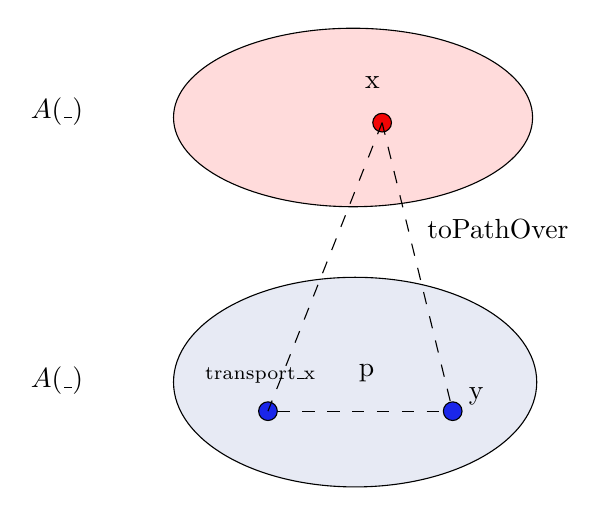
\begin{tikzpicture}[x=0.75pt,y=0.75pt,yscale=-1,xscale=1]
%uncomment if require: \path (0,300); %set diagram left start at 0, and has height of 300

%Shape: Ellipse [id:dp6858943436655307]
\draw  [fill={rgb, 255:red, 231; green, 234; blue, 244 }  ,fill opacity=1 ] (230,230.5) .. controls (230,202.61) and (269.18,180) .. (317.5,180) .. controls (365.82,180) and (405,202.61) .. (405,230.5) .. controls (405,258.39) and (365.82,281) .. (317.5,281) .. controls (269.18,281) and (230,258.39) .. (230,230.5) -- cycle ;
%Shape: Ellipse [id:dp4978096684614166]
\draw  [fill={rgb, 255:red, 255; green, 219; blue, 219 }  ,fill opacity=1 ] (230,103) .. controls (230,79.25) and (268.73,60) .. (316.5,60) .. controls (364.27,60) and (403,79.25) .. (403,103) .. controls (403,126.75) and (364.27,146) .. (316.5,146) .. controls (268.73,146) and (230,126.75) .. (230,103) -- cycle ;
%Shape: Circle [id:dp2462377080592002]
\draw  [fill={rgb, 255:red, 242; green, 5; blue, 5 }  ,fill opacity=1 ] (326,105.5) .. controls (326,103.01) and (328.01,101) .. (330.5,101) .. controls (332.99,101) and (335,103.01) .. (335,105.5) .. controls (335,107.99) and (332.99,110) .. (330.5,110) .. controls (328.01,110) and (326,107.99) .. (326,105.5) -- cycle ;
%Shape: Circle [id:dp1552015327211651]
\draw  [fill={rgb, 255:red, 26; green, 38; blue, 234 }  ,fill opacity=1 ] (360,244.5) .. controls (360,242.01) and (362.01,240) .. (364.5,240) .. controls (366.99,240) and (369,242.01) .. (369,244.5) .. controls (369,246.99) and (366.99,249) .. (364.5,249) .. controls (362.01,249) and (360,246.99) .. (360,244.5) -- cycle ;
%Shape: Circle [id:dp924511868212545]
\draw  [fill={rgb, 255:red, 26; green, 38; blue, 234 }  ,fill opacity=1 ] (271,244.5) .. controls (271,242.01) and (273.01,240) .. (275.5,240) .. controls (277.99,240) and (280,242.01) .. (280,244.5) .. controls (280,246.99) and (277.99,249) .. (275.5,249) .. controls (273.01,249) and (271,246.99) .. (271,244.5) -- cycle ;
%Straight Lines [id:da43777492366231496]
\draw  [dash pattern={on 4.5pt off 4.5pt}]  (280,244.5) -- (360,244.5) ;
%Straight Lines [id:da5251303335065973]
\draw  [dash pattern={on 4.5pt off 4.5pt}]  (330.5,105.5) -- (364.5,244.5) ;
%Straight Lines [id:da2553652396779533]
\draw  [dash pattern={on 4.5pt off 4.5pt}]  (330.5,105.5) -- (275.5,244.5) ;

% Text Node
\draw (321,82) node [anchor=north west][inner sep=0.75pt]   [align=left] {x};
% Text Node
\draw (371,232) node [anchor=north west][inner sep=0.75pt]   [align=left] {y};
% Text Node
\draw (244,222) node [anchor=north west][inner sep=0.75pt]  [font=\scriptsize] [align=left] {transport\_x};
% Text Node
\draw (318,221) node [anchor=north west][inner sep=0.75pt]   [align=left] {p};
% Text Node
\draw (160,92) node [anchor=north west][inner sep=0.75pt]   [align=left] {$\Funapp{\id{A}}{(\earg{\_}{\ileft})}$};
% Text Node
\draw (160,222) node [anchor=north west][inner sep=0.75pt]   [align=left] {$\Funapp{\id{A}}{(\earg{\_}{\iright})}$};
% Text Node
\draw (351,150.92) node [anchor=north west][inner sep=0.75pt]  [rotate=-0.06] [align=left] {toPathOver};

\end{tikzpicture}
\end{center}

The circles represent the two types and points in the circle are elements of the corresponding types. With our definition of equality, we can trivially construct an equality between $\Funapp{\id{A}}{(\earg{\_}{\ileft})}$ and $\Funapp{\id{A}}{(\earg{\_}{\iright})}$. Now, given that the two circles are `equal', intuitively speaking, every point in one circle should have a counterpart in the other circle, and this can be obtained transporting a point along the equality between the two types. The result of transporting $\id{x}$ to the type $\Funapp{\id{A}}{(\earg{\_}{\iright})}$ is a point that we shall call $\id{transport\_x}$. Additionally, suppose also that we have an equality between $\id{transport\_x}$ and $\id{y}$, this is indicated by the path $\id{p}$ between the two points in the diagram. Given that $\id{x}$ is transported to $\id{transport\_x}$, and that $\id{transport\_x}$ is equal to $\id{y}$, we also want to be able to say something about the relationship between $\id{x}$ and $\id{y}$. Since they are not of the same type, all we can do is construct a heterogenous equality between them, and this is precisely what the function $\id{toPathOver}$ seeks to do.

\begin{minted}[escapeinside=@@,mathescape=true]{haskell}
toPathOver : (A : I @$\Rrightarrow$@ Type) @$\Rrightarrow$@ (x : A (_ := i0)) @$\Rightarrow$@ (y : A (_ := i1))
             @$\Rightarrow$@ Eq (Eq_cast (p := Eq_eq (f := A)) (f := id) x) y
             @$\rightarrow$@ Heq x y;
toPathOver = @$\lambda$@ _  A @$\Rrightarrow$@ @$\lambda$@ x y @$\Rightarrow$@ @$\lambda$@ p @$\rightarrow$@
  let
    l : Heq x (Eq_cast (p := Eq_eq (f := A)) (f := id) x);
    l = Heq_eq (t := A)
               (f := @$\lambda$@ i @$\Rrightarrow$@
                     I_transp (A := (@$\lambda$@ j @$\Rrightarrow$@ A (_ := I_meet i j)))
                              (r := I_not i) x);
  in
    Eq_cast
        (x := (Eq_cast (p := Eq_eq (f := A)) (f := id) x))
        (y := y)
        (p := p) (f := @$\lambda$@ y' @$\rightarrow$@ Heq x y') l;
\end{minted}

We construct a heterogenous equality between $\id{x}$ and $\id{transport\_x}$ and we concatenate it with the equality proof between $\id{transport\_x}$ and $\id{y}$ to complete the proof.

\begin{minted}[escapeinside=@@,mathescape=true]{haskell}
elimProp : (A : Type_ ?) @$\Rrightarrow$@ (R : A @$\rightarrow$@ A @$\rightarrow$@ Type)
           @$\Rrightarrow$@ (P : Quotient A R @$\rightarrow$@ Type)
           @$\Rrightarrow$@ (prop : (x : Quotient A R) @$\rightarrow$@ isProp (P x))
           @$\rightarrow$@ (f : (x : A) @$\rightarrow$@ P (Quotient_in x))
           @$\rightarrow$@ (x : Quotient A R) @$\rightarrow$@ P x
elimProp = @$\lambda$@ _ _ _ A R P @$\Rrightarrow$@ @$\lambda$@ prop f @$\rightarrow$@
  Quotient_elim
    (R := R) (P := P) f
    (p := @$\lambda$@ a a' r @$\rightarrow$@
      let
        a=a' : Eq (t := Quotient A R) (Quotient_in a) (Quotient_in a')
        a=a' = Quotient_eq (R := R) (a := a) (a' := a') r
        fa=fa' : Heq (f a) (f a')
        fa=fa' = toPathOver
                    (A := @$\lambda$@ i @$\Rrightarrow$@ P (Eq_uneq (p := a=a') (i := i)))
                    (prop (Quotient_in a')
                          (Eq_cast (p := a=a') (f := P) (f a))
                          (f a'))
      in
        fa=fa')
\end{minted}

$\fn{toPathOver}$ does the heavy lifting in this proof by allowing us to leverage $\Funapp{\fn{isProp}}{(\Funapp{\id{P}}{\id{x}})}$ to easily produce a proof of $\Funapp{\id{Heq}}{(\Funapp{\id{f}}{\id{a}})}{(\Funapp{\id{f}}{\id{a}'})}$. We can also iterate this to define $\fn{elimProp}_2$, $\fn{elimProp}_3$ etc. In general, we can define $\fn{elimProp}_n$ in terms of $\fn{elimProp}_{n-1}$ and $\fn{elimProp}$. To illustrate this, we define $\fn{elimProp}_2$.

\begin{minted}[escapeinside=@@,mathescape=true]{haskell}
elimProp2 : (A B : Type)
            @$\Rrightarrow$@ (R : A @$\rightarrow$@ A @$\rightarrow$@ Type) @$\Rrightarrow$@ (S : B @$\rightarrow$@ B @$\rightarrow$@ Type)
            @$\Rrightarrow$@ (P : Quotient A R @$\rightarrow$@ Quotient B S @$\rightarrow$@ Type)
            @$\Rrightarrow$@ (prop : (x : Quotient A R) @$\rightarrow$@ (y : Quotient B S)
                       @$\rightarrow$@ isProp (P x y))
            @$\rightarrow$@ (f : (x : A) @$\rightarrow$@ (y : B) @$\rightarrow$@ P (Quotient_in x) (Quotient_in y))
            @$\rightarrow$@ (x : Quotient A R) @$\rightarrow$@ (y : Quotient B S) @$\rightarrow$@ P x y
elimProp2 = @$\lambda$@ _ _ _ _ _ A B R S P @$\Rrightarrow$@ @$\lambda$@ prop f @$\rightarrow$@
  elimProp (P := @$\lambda$@ x @$\rightarrow$@ (y : Quotient B S) @$\rightarrow$@ P x y)
           (@$\lambda$@ x @$\rightarrow$@ isProp@$\Pi$@ (B := P x) (prop x))
           (@$\lambda$@ a @$\rightarrow$@ elimProp (P := P (Quotient_in a))
                            (prop (Quotient_in a)) (f a))
\end{minted}

TODO\: Consider defining a macro that defines $\fn{elimProp}_n$, i.e.\ the general case.

\chapter{Holy Trinity?}
There is an intricate relationship between logic, programming (type theory) and category theory, as was proposed by Harper (TODO:\ link his article https://existentialtype.wordpress.com/2011/03/27/the-holy-trinity/). Everything that exists in each of these domains necessarily has an interesting analogue in the other two. In this chapter, we discuss quotients from the perspective of logic and category theory. In some cases, this will motivate the `discovery' of some interesting properties of the $\kw{Quotient}$ type.

\section{Relationship to Logic}
TODO:\ Figure out what could be informative to say here.

\section{Relationship to Category Theory}
%% TODO: Maybe I should reconsider how much value is added by having this here
%% honestly, I'm starting to have second thoughts... If this can inspire a few
%% interesting theorems out about Quotient types it'd be more interesting

Numerous constructs in type theory have equivalents in category theory. To set the stage for this, we shall do a very short primer on category theory. For a more detailed introduction, interested readers are directed to other works such as Awodey's textbook\cite{awodey-cattheory}.

\subsection{Introduction}
Category theory is built on merely a few foundational constructs, these alone give rise to a lot of interesting structures and properties. First, we postulate the existence of categories that contain objects. Next, we say that objects can be related to other objects via morphisms (also known as arrows, these two terms shall be used interchangeably in the following discussion). Assuming that readers are familiar with programming and/or type theory, one could think of categories as types, objects as terms of a particular type, and morphisms as functions. Every object has an identity arrow that relates it with itself.

\begin{figure}[H]
\centering
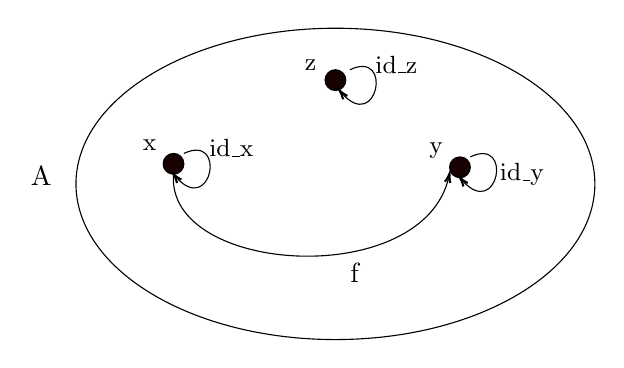
\begin{tikzpicture}[x=0.75pt,y=0.75pt,yscale=-1,xscale=1]
%uncomment if require: \path (0,300); %set diagram left start at 0, and has height of 300

%Shape: Ellipse [id:dp9346439808655433]
\draw   (220,155) .. controls (220,113.58) and (275.96,80) .. (345,80) .. controls (414.04,80) and (470,113.58) .. (470,155) .. controls (470,196.42) and (414.04,230) .. (345,230) .. controls (275.96,230) and (220,196.42) .. (220,155) -- cycle ;
%Shape: Circle [id:dp22784360669527182]
\draw  [fill={rgb, 255:red, 23; green, 1; blue, 1 }  ,fill opacity=1 ] (262,145.33) .. controls (262,142.56) and (264.24,140.33) .. (267,140.33) .. controls (269.76,140.33) and (272,142.56) .. (272,145.33) .. controls (272,148.09) and (269.76,150.33) .. (267,150.33) .. controls (264.24,150.33) and (262,148.09) .. (262,145.33) -- cycle ;
%Curve Lines [id:da27074905740711297]
\draw    (272,140.33) .. controls (292.91,130.36) and (285.32,171.14) .. (268.07,151.6) ;
\draw [shift={(267,150.33)}, rotate = 51.34] [color={rgb, 255:red, 0; green, 0; blue, 0 }  ][line width=0.75]    (4.37,-1.32) .. controls (2.78,-0.56) and (1.32,-0.12) .. (0,0) .. controls (1.32,0.12) and (2.78,0.56) .. (4.37,1.32)   ;
%Shape: Circle [id:dp9211255412324888]
\draw  [fill={rgb, 255:red, 23; green, 1; blue, 1 }  ,fill opacity=1 ] (400,147) .. controls (400,144.24) and (402.24,142) .. (405,142) .. controls (407.76,142) and (410,144.24) .. (410,147) .. controls (410,149.76) and (407.76,152) .. (405,152) .. controls (402.24,152) and (400,149.76) .. (400,147) -- cycle ;
%Curve Lines [id:da7233344958507704]
\draw    (410,142) .. controls (430.91,132.04) and (423.32,172.81) .. (406.07,153.27) ;
\draw [shift={(405,152)}, rotate = 51.34] [color={rgb, 255:red, 0; green, 0; blue, 0 }  ][line width=0.75]    (4.37,-1.32) .. controls (2.78,-0.56) and (1.32,-0.12) .. (0,0) .. controls (1.32,0.12) and (2.78,0.56) .. (4.37,1.32)   ;
%Curve Lines [id:da38568823352847637]
\draw    (267,150.33) .. controls (263.04,198.67) and (387.15,206.66) .. (399.66,151.69) ;
\draw [shift={(400,150)}, rotate = 102.82] [color={rgb, 255:red, 0; green, 0; blue, 0 }  ][line width=0.75]    (4.37,-1.32) .. controls (2.78,-0.56) and (1.32,-0.12) .. (0,0) .. controls (1.32,0.12) and (2.78,0.56) .. (4.37,1.32)   ;
%Shape: Circle [id:dp8096171242464965]
\draw  [fill={rgb, 255:red, 23; green, 1; blue, 1 }  ,fill opacity=1 ] (340,105) .. controls (340,102.24) and (342.24,100) .. (345,100) .. controls (347.76,100) and (350,102.24) .. (350,105) .. controls (350,107.76) and (347.76,110) .. (345,110) .. controls (342.24,110) and (340,107.76) .. (340,105) -- cycle ;
%Curve Lines [id:da10314349904359177]
\draw    (352,100) .. controls (372.91,90.04) and (365.32,130.81) .. (348.07,111.27) ;
\draw [shift={(347,110)}, rotate = 51.34] [color={rgb, 255:red, 0; green, 0; blue, 0 }  ][line width=0.75]    (4.37,-1.32) .. controls (2.78,-0.56) and (1.32,-0.12) .. (0,0) .. controls (1.32,0.12) and (2.78,0.56) .. (4.37,1.32)   ;

% Text Node
\draw (197,145.5) node [anchor=north west][inner sep=0.75pt]   [align=left] {A};
% Text Node
\draw (251,132.33) node [anchor=north west][inner sep=0.75pt]  [font=\small] [align=left] {x};
% Text Node
\draw (283,132.33) node [anchor=north west][inner sep=0.75pt]  [font=\small] [align=left] {id\_x};
% Text Node
\draw (389,134) node [anchor=north west][inner sep=0.75pt]  [font=\small] [align=left] {y};
% Text Node
\draw (423,144) node [anchor=north west][inner sep=0.75pt]  [font=\small] [align=left] {id\_y};
% Text Node
\draw (351,192) node [anchor=north west][inner sep=0.75pt]   [align=left] {f};
% Text Node
\draw (363,92) node [anchor=north west][inner sep=0.75pt]  [font=\small] [align=left] {id\_z};
% Text Node
\draw (329,94) node [anchor=north west][inner sep=0.75pt]  [font=\small] [align=left] {z};


\end{tikzpicture}
\caption{Example of a category A with objects x, y and z with a morphism f that goes from x to y}
\end{figure}

At the heart of category theory, we have the notion of composition. Suppose that we have an arrow from A to B, and another arrow from B to C, then there is necessarily another arrow that goes directly from A to C. We call this the composition of the first two arrows. This is of course analogous to function composition in programming.

\begin{figure}[H]
\centering

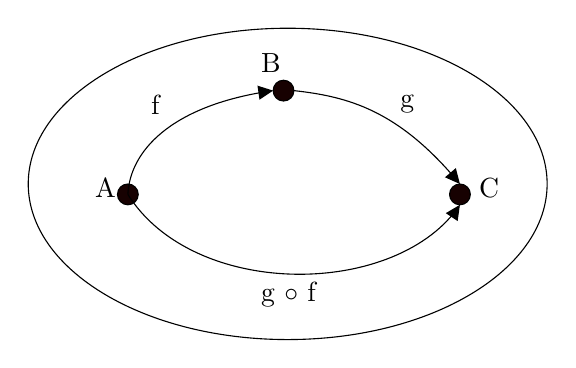
\begin{tikzpicture}[x=0.75pt,y=0.75pt,yscale=-1,xscale=1]
%uncomment if require: \path (0,300); %set diagram left start at 0, and has height of 300

%Shape: Ellipse [id:dp5682347326089148]
\draw   (210,155) .. controls (210,113.58) and (265.96,80) .. (335,80) .. controls (404.04,80) and (460,113.58) .. (460,155) .. controls (460,196.42) and (404.04,230) .. (335,230) .. controls (265.96,230) and (210,196.42) .. (210,155) -- cycle ;
%Shape: Circle [id:dp9592501831446234]
\draw  [fill={rgb, 255:red, 23; green, 1; blue, 1 }  ,fill opacity=1 ] (253,160.06) .. controls (253,157.3) and (255.24,155.06) .. (258,155.06) .. controls (260.76,155.06) and (263,157.3) .. (263,160.06) .. controls (263,162.82) and (260.76,165.06) .. (258,165.06) .. controls (255.24,165.06) and (253,162.82) .. (253,160.06) -- cycle ;
%Shape: Circle [id:dp2931536659208638]
\draw  [fill={rgb, 255:red, 23; green, 1; blue, 1 }  ,fill opacity=1 ] (328,110.06) .. controls (328,107.3) and (330.24,105.06) .. (333,105.06) .. controls (335.76,105.06) and (338,107.3) .. (338,110.06) .. controls (338,112.82) and (335.76,115.06) .. (333,115.06) .. controls (330.24,115.06) and (328,112.82) .. (328,110.06) -- cycle ;
%Curve Lines [id:da24285465512107507]
\draw    (338,110.06) .. controls (364.46,112.94) and (388.04,119.72) .. (416.27,152.99) ;
\draw [shift={(418,155.06)}, rotate = 229.87] [fill={rgb, 255:red, 0; green, 0; blue, 0 }  ][line width=0.08]  [draw opacity=0] (7.14,-3.43) -- (0,0) -- (7.14,3.43) -- cycle    ;
%Curve Lines [id:da2451569195346175]
\draw    (258,160.06) .. controls (258.98,139.48) and (278.21,117.88) .. (325.09,110.49) ;
\draw [shift={(328,110.06)}, rotate = 171.94] [fill={rgb, 255:red, 0; green, 0; blue, 0 }  ][line width=0.08]  [draw opacity=0] (7.14,-3.43) -- (0,0) -- (7.14,3.43) -- cycle    ;
%Shape: Circle [id:dp5266322522520346]
\draw  [fill={rgb, 255:red, 23; green, 1; blue, 1 }  ,fill opacity=1 ] (413,160.06) .. controls (413,157.3) and (415.24,155.06) .. (418,155.06) .. controls (420.76,155.06) and (423,157.3) .. (423,160.06) .. controls (423,162.82) and (420.76,165.06) .. (418,165.06) .. controls (415.24,165.06) and (413,162.82) .. (413,160.06) -- cycle ;
%Curve Lines [id:da19962913311880914]
\draw    (258,160.06) .. controls (289.52,210.24) and (385.07,210.02) .. (416.6,167.05) ;
\draw [shift={(418,165.06)}, rotate = 123.72] [fill={rgb, 255:red, 0; green, 0; blue, 0 }  ][line width=0.08]  [draw opacity=0] (7.14,-3.43) -- (0,0) -- (7.14,3.43) -- cycle    ;

% Text Node
\draw (321,91) node [anchor=north west][inner sep=0.75pt]   [align=left] {B};
% Text Node
\draw (241,151) node [anchor=north west][inner sep=0.75pt]   [align=left] {A};
% Text Node
\draw (426,151) node [anchor=north west][inner sep=0.75pt]   [align=left] {C};
% Text Node
\draw (268,111) node [anchor=north west][inner sep=0.75pt]   [align=left] {f};
% Text Node
\draw (388,111) node [anchor=north west][inner sep=0.75pt]   [align=left] {g};
% Text Node
\draw (321,201) node [anchor=north west][inner sep=0.75pt]   [align=left] {g $\circ$ f};

\end{tikzpicture}

\caption{The composition of two morphisms f and g. The identity arrows are not explicitly shown as we can take their existence for granted.}

\end{figure}

To conclude our short introduction to category theory, we would like to present the category theoretic equivalent of a ubiqituous construct in type theory, i.e.\ products (also known as tuples). One should be familiar with the notion of products being defined as pairs of elements, however in category theory, we have to define such objects in terms of its morphisms that relate it to other objects. If some object C were to be the product of objects A and B, then we require that it has two morphisms that behave as the first and second projections out of the product. In other words, we require the two morphisms $\id{p} : \id{C} \rightarrow \id{A}$ and $\id{q} : \id{C} \rightarrow \id{B}$.

\begin{figure}[H]
  \centering

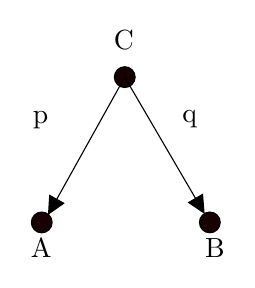
\begin{tikzpicture}[x=0.75pt,y=0.75pt,yscale=-1,xscale=1]
%uncomment if require: \path (0,300); %set diagram left start at 0, and has height of 300

%Shape: Circle [id:dp07095704485213461]
\draw  [fill={rgb, 255:red, 23; green, 1; blue, 1 }  ,fill opacity=1 ] (339.5,95.06) .. controls (339.5,92.3) and (341.74,90.06) .. (344.5,90.06) .. controls (347.26,90.06) and (349.5,92.3) .. (349.5,95.06) .. controls (349.5,97.82) and (347.26,100.06) .. (344.5,100.06) .. controls (341.74,100.06) and (339.5,97.82) .. (339.5,95.06) -- cycle ;
%Shape: Circle [id:dp6029113112328306]
\draw  [fill={rgb, 255:red, 23; green, 1; blue, 1 }  ,fill opacity=1 ] (380.5,165.06) .. controls (380.5,162.3) and (382.74,160.06) .. (385.5,160.06) .. controls (388.26,160.06) and (390.5,162.3) .. (390.5,165.06) .. controls (390.5,167.82) and (388.26,170.06) .. (385.5,170.06) .. controls (382.74,170.06) and (380.5,167.82) .. (380.5,165.06) -- cycle ;
%Shape: Circle [id:dp8272191866621565]
\draw  [fill={rgb, 255:red, 23; green, 1; blue, 1 }  ,fill opacity=1 ] (299.5,165.06) .. controls (299.5,162.3) and (301.74,160.06) .. (304.5,160.06) .. controls (307.26,160.06) and (309.5,162.3) .. (309.5,165.06) .. controls (309.5,167.82) and (307.26,170.06) .. (304.5,170.06) .. controls (301.74,170.06) and (299.5,167.82) .. (299.5,165.06) -- cycle ;
%Straight Lines [id:da6629962247946746]
\draw    (344.5,95.06) -- (308.96,158.88) ;
\draw [shift={(307.5,161.5)}, rotate = 299.11] [fill={rgb, 255:red, 0; green, 0; blue, 0 }  ][line width=0.08]  [draw opacity=0] (8.93,-4.29) -- (0,0) -- (8.93,4.29) -- cycle    ;
%Straight Lines [id:da8118877575329375]
\draw    (344.5,95.06) -- (381.49,158.41) ;
\draw [shift={(383,161)}, rotate = 239.72] [fill={rgb, 255:red, 0; green, 0; blue, 0 }  ][line width=0.08]  [draw opacity=0] (8.93,-4.29) -- (0,0) -- (8.93,4.29) -- cycle    ;

% Text Node
\draw (338,71.5) node [anchor=north west][inner sep=0.75pt]   [align=left] {C};
% Text Node
\draw (382,171.5) node [anchor=north west][inner sep=0.75pt]   [align=left] {B};
% Text Node
\draw (298,171.5) node [anchor=north west][inner sep=0.75pt]   [align=left] {A};
% Text Node
\draw (299,110.5) node [anchor=north west][inner sep=0.75pt]   [align=left] {p};
% Text Node
\draw (371,110) node [anchor=north west][inner sep=0.75pt]   [align=left] {q};

\end{tikzpicture}

\caption{A candidate product of A and B with its projection morphisms.}

\end{figure}

However, we notice that this is far too general of a definition since it is likely that there are many objects that fulfil these criteria. Here, we introduce the notion of a universal property which allows us to identify `the best product'. The best product is the one that is not too general, and yet not too restrictive, it is `just right'. More formally, the product of $\id{A}$ and $\id{B}$ is an object $\id{A} \times \id{B}$ with the morphisms $\pi_1 : \id{A} \times \id{B} \rightarrow A$ and $\pi_2 : \id{A} \times \id{B} \rightarrow B$. Additionally, for any other object $\id{C}$ with morphisms $\id{p} : \id{C} \rightarrow \id{A}$ and $\id{q} : \id{C} \rightarrow \id{B}$, there exists a unique morphism $\id{f}$ such that $\id{p} = \pi_1 \circ \id{f}$ and $\id{q} = \pi_2 \circ \id{f}$. In other words, we require that the following diagram commute:

\begin{figure}[H]
\centering

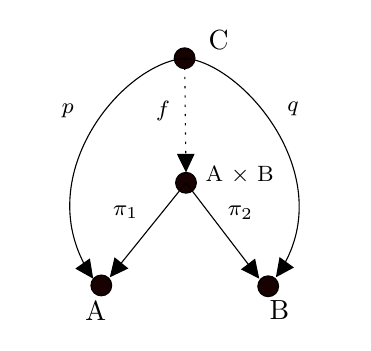
\begin{tikzpicture}[x=0.75pt,y=0.75pt,yscale=-1,xscale=1]
%uncomment if require: \path (0,300); %set diagram left start at 0, and has height of 300

%Shape: Circle [id:dp8623415585531431]
\draw  [fill={rgb, 255:red, 23; green, 1; blue, 1 }  ,fill opacity=1 ] (350.7,165.46) .. controls (350.7,162.7) and (352.94,160.46) .. (355.7,160.46) .. controls (358.46,160.46) and (360.7,162.7) .. (360.7,165.46) .. controls (360.7,168.22) and (358.46,170.46) .. (355.7,170.46) .. controls (352.94,170.46) and (350.7,168.22) .. (350.7,165.46) -- cycle ;
%Shape: Circle [id:dp8629465911347864]
\draw  [fill={rgb, 255:red, 23; green, 1; blue, 1 }  ,fill opacity=1 ] (309.9,214.92) .. controls (309.9,212.16) and (312.14,209.92) .. (314.9,209.92) .. controls (317.66,209.92) and (319.9,212.16) .. (319.9,214.92) .. controls (319.9,217.69) and (317.66,219.92) .. (314.9,219.92) .. controls (312.14,219.92) and (309.9,217.69) .. (309.9,214.92) -- cycle ;
%Shape: Circle [id:dp07686054824860356]
\draw  [fill={rgb, 255:red, 23; green, 1; blue, 1 }  ,fill opacity=1 ] (390.3,215.32) .. controls (390.3,212.56) and (392.54,210.32) .. (395.3,210.32) .. controls (398.06,210.32) and (400.3,212.56) .. (400.3,215.32) .. controls (400.3,218.09) and (398.06,220.32) .. (395.3,220.32) .. controls (392.54,220.32) and (390.3,218.09) .. (390.3,215.32) -- cycle ;
%Straight Lines [id:da5396059636931949]
\draw    (355.7,165.46) -- (320.88,208.66) ;
\draw [shift={(319,211)}, rotate = 308.86] [fill={rgb, 255:red, 0; green, 0; blue, 0 }  ][line width=0.08]  [draw opacity=0] (8.93,-4.29) -- (0,0) -- (8.93,4.29) -- cycle    ;
%Straight Lines [id:da09985777044473254]
\draw    (355.7,165.46) -- (389.18,209.28) ;
\draw [shift={(391,211.67)}, rotate = 232.62] [fill={rgb, 255:red, 0; green, 0; blue, 0 }  ][line width=0.08]  [draw opacity=0] (8.93,-4.29) -- (0,0) -- (8.93,4.29) -- cycle    ;
%Shape: Circle [id:dp44714117032868783]
\draw  [fill={rgb, 255:red, 23; green, 1; blue, 1 }  ,fill opacity=1 ] (350.03,105.46) .. controls (350.03,102.7) and (352.27,100.46) .. (355.03,100.46) .. controls (357.79,100.46) and (360.03,102.7) .. (360.03,105.46) .. controls (360.03,108.22) and (357.79,110.46) .. (355.03,110.46) .. controls (352.27,110.46) and (350.03,108.22) .. (350.03,105.46) -- cycle ;
%Curve Lines [id:da13360932709149242]
\draw    (355.03,105.46) .. controls (324.14,108.29) and (279.69,163.31) .. (309.58,209.56) ;
\draw [shift={(311,211.67)}, rotate = 235.01] [fill={rgb, 255:red, 0; green, 0; blue, 0 }  ][line width=0.08]  [draw opacity=0] (8.93,-4.29) -- (0,0) -- (8.93,4.29) -- cycle    ;
%Curve Lines [id:da35945481458004735]
\draw    (355.03,105.46) .. controls (383.24,107.63) and (430.88,163.29) .. (400.44,208.92) ;
\draw [shift={(399,211)}, rotate = 305.93] [fill={rgb, 255:red, 0; green, 0; blue, 0 }  ][line width=0.08]  [draw opacity=0] (8.93,-4.29) -- (0,0) -- (8.93,4.29) -- cycle    ;
%Straight Lines [id:da17703597924842862]
\draw  [dash pattern={on 0.84pt off 2.51pt}]  (355.03,105.46) -- (355.66,157.46) ;
\draw [shift={(355.7,160.46)}, rotate = 269.31] [fill={rgb, 255:red, 0; green, 0; blue, 0 }  ][line width=0.08]  [draw opacity=0] (8.93,-4.29) -- (0,0) -- (8.93,4.29) -- cycle    ;

% Text Node
\draw (363.87,156.33) node [anchor=north west][inner sep=0.75pt]  [font=\footnotesize] [align=left] {A $\times$ B};
% Text Node
\draw (306,221.67) node [anchor=north west][inner sep=0.75pt]   [align=left] {A};
% Text Node
\draw (394.67,221) node [anchor=north west][inner sep=0.75pt]   [align=left] {B};
% Text Node
\draw (319.33,175.33) node [anchor=north west][inner sep=0.75pt]  [font=\footnotesize] [align=left] {$\displaystyle \pi _{1}$};
% Text Node
\draw (374.67,175.6) node [anchor=north west][inner sep=0.75pt]  [font=\footnotesize] [align=left] {$\displaystyle \pi _{2}$};
% Text Node
\draw (365.33,91) node [anchor=north west][inner sep=0.75pt]   [align=left] {C};
% Text Node
\draw (294.67,126) node [anchor=north west][inner sep=0.75pt]  [font=\footnotesize] [align=left] {$\displaystyle p$};
% Text Node
\draw (403.33,125.33) node [anchor=north west][inner sep=0.75pt]  [font=\footnotesize] [align=left] {$\displaystyle q$};
% Text Node
\draw (340,124.67) node [anchor=north west][inner sep=0.75pt]  [font=\footnotesize] [align=left] {$\displaystyle f$};

\end{tikzpicture}

\caption{Universal mapping property of the product}

\end{figure}

Another way of saying the above is that $\id{h}$ factorises $\id{p}$ and $\id{q}$. The universal product, if it exists, is unique up to isomorphism. Products are not guaranteed to exist in every category. In the category of sets, the universal product is none other than the Cartesian product.

\subsection{Coequaliser}
We now introduce the notion of a coequaliser. We shall see later that $\kw{Quotient}$ acts indeed as a coequaliser, or rather coequalisers are generalisation of quotients. For two arrows $\oftype{f, g}{A \rightarrow B}$, a coequaliser is an arrow $\oftype{q}{B \rightarrow Q}$ such that $qf = qg$ (we use juxtaposition to imply composition). The universal property of the coequaliser then dictates that for any other $Z$ and $\oftype{z}{B \rightarrow Z}$, if $zf = zg$, then there must exist a unique $\oftype{u}{Q \rightarrow Z}$ such that $uq = g$. This allows us to call $q$ \textbf{the} coequaliser of $f$ and $g$.

\begin{figure}[H]
  \centering
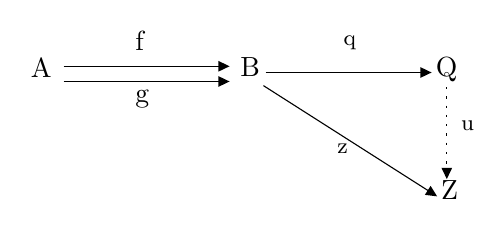
\begin{tikzpicture}[x=0.75pt,y=0.75pt,yscale=-1,xscale=1]
%uncomment if require: \path (0,300); %set diagram left start at 0, and has height of 300

%Straight Lines [id:da9967367962188358]
\draw    (208,127) -- (285,127) ;
\draw [shift={(288,127)}, rotate = 180] [fill={rgb, 255:red, 0; green, 0; blue, 0 }  ][line width=0.08]  [draw opacity=0] (5.36,-2.57) -- (0,0) -- (5.36,2.57) -- cycle    ;
%Straight Lines [id:da10808455754917401]
\draw    (208,134.33) -- (285,134.33) ;
\draw [shift={(288,134.33)}, rotate = 180] [fill={rgb, 255:red, 0; green, 0; blue, 0 }  ][line width=0.08]  [draw opacity=0] (5.36,-2.57) -- (0,0) -- (5.36,2.57) -- cycle    ;
%Straight Lines [id:da5630721975359221]
\draw    (305.33,130) -- (382.33,130) ;
\draw [shift={(385.33,130)}, rotate = 180] [fill={rgb, 255:red, 0; green, 0; blue, 0 }  ][line width=0.08]  [draw opacity=0] (5.36,-2.57) -- (0,0) -- (5.36,2.57) -- cycle    ;
%Straight Lines [id:da6026678626663149]
\draw    (304.33,136.33) -- (385.47,188.05) ;
\draw [shift={(388,189.67)}, rotate = 212.52] [fill={rgb, 255:red, 0; green, 0; blue, 0 }  ][line width=0.08]  [draw opacity=0] (5.36,-2.57) -- (0,0) -- (5.36,2.57) -- cycle    ;
%Straight Lines [id:da1216641628607622]
\draw  [dash pattern={on 0.84pt off 2.51pt}]  (392.67,137) -- (392.67,178.33) ;
\draw [shift={(392.67,181.33)}, rotate = 270] [fill={rgb, 255:red, 0; green, 0; blue, 0 }  ][line width=0.08]  [draw opacity=0] (5.36,-2.57) -- (0,0) -- (5.36,2.57) -- cycle    ;

% Text Node
\draw (191,122) node [anchor=north west][inner sep=0.75pt]  [font=\normalsize] [align=left] {A};
% Text Node
\draw (292,121.5) node [anchor=north west][inner sep=0.75pt]   [align=left] {B};
% Text Node
\draw (386.17,121.67) node [anchor=north west][inner sep=0.75pt]   [align=left] {Q};
% Text Node
\draw (388.67,181) node [anchor=north west][inner sep=0.75pt]   [align=left] {Z};
% Text Node
\draw (241.33,108.67) node [anchor=north west][inner sep=0.75pt]   [align=left] {f};
% Text Node
\draw (241.33,137.33) node [anchor=north west][inner sep=0.75pt]   [align=left] {g};
% Text Node
\draw (341.67,111) node [anchor=north west][inner sep=0.75pt]  [font=\footnotesize] [align=left] {q};
% Text Node
\draw (338.67,163) node [anchor=north west][inner sep=0.75pt]  [font=\footnotesize] [align=left] {z};
% Text Node
\draw (398.33,152) node [anchor=north west][inner sep=0.75pt]  [font=\footnotesize] [align=left] {u};


\end{tikzpicture}

\caption{Illustration of a coequaliser}

\end{figure}

\textbf{Proposition} In any category, if $\oftype{q}{B \rightarrow Q}$ is a coequaliser of a pair of arrows $\oftype{f, \ g}{A \rightarrow B}$, then $q$ is an epimorphism.

Proof.

We first state the definition of an epimorphism. An epimorphism is a morphism $\oftype{f}{X \rightarrow Y}$ such that for all objects C and morphisms $\oftype{g_1, g_2}{Y \rightarrow Z}$, if $g_1f = g_2f$ then $g_1 = g_2$.

Now, we consider the below diagram

\begin{figure}[H]
  \centering
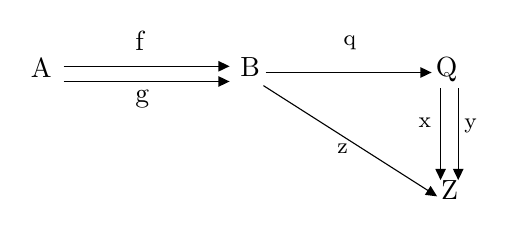
\begin{tikzpicture}[x=0.75pt,y=0.75pt,yscale=-1,xscale=1]
%uncomment if require: \path (0,300); %set diagram left start at 0, and has height of 300

%Straight Lines [id:da5779265165541632]
\draw    (208,127) -- (285,127) ;
\draw [shift={(288,127)}, rotate = 180] [fill={rgb, 255:red, 0; green, 0; blue, 0 }  ][line width=0.08]  [draw opacity=0] (5.36,-2.57) -- (0,0) -- (5.36,2.57) -- cycle    ;
%Straight Lines [id:da20539623997737722]
\draw    (208,134.33) -- (285,134.33) ;
\draw [shift={(288,134.33)}, rotate = 180] [fill={rgb, 255:red, 0; green, 0; blue, 0 }  ][line width=0.08]  [draw opacity=0] (5.36,-2.57) -- (0,0) -- (5.36,2.57) -- cycle    ;
%Straight Lines [id:da259761440148945]
\draw    (305.33,130) -- (382.33,130) ;
\draw [shift={(385.33,130)}, rotate = 180] [fill={rgb, 255:red, 0; green, 0; blue, 0 }  ][line width=0.08]  [draw opacity=0] (5.36,-2.57) -- (0,0) -- (5.36,2.57) -- cycle    ;
%Straight Lines [id:da923412514180374]
\draw    (304.33,136.33) -- (385.47,188.05) ;
\draw [shift={(388,189.67)}, rotate = 212.52] [fill={rgb, 255:red, 0; green, 0; blue, 0 }  ][line width=0.08]  [draw opacity=0] (5.36,-2.57) -- (0,0) -- (5.36,2.57) -- cycle    ;
%Straight Lines [id:da6028721128255661]
\draw    (389.67,137.5) -- (389.67,178.83) ;
\draw [shift={(389.67,181.83)}, rotate = 270] [fill={rgb, 255:red, 0; green, 0; blue, 0 }  ][line width=0.08]  [draw opacity=0] (5.36,-2.57) -- (0,0) -- (5.36,2.57) -- cycle    ;
%Straight Lines [id:da20084318131652013]
\draw    (398.17,137.5) -- (398.17,178.83) ;
\draw [shift={(398.17,181.83)}, rotate = 270] [fill={rgb, 255:red, 0; green, 0; blue, 0 }  ][line width=0.08]  [draw opacity=0] (5.36,-2.57) -- (0,0) -- (5.36,2.57) -- cycle    ;

% Text Node
\draw (191,122) node [anchor=north west][inner sep=0.75pt]  [font=\normalsize] [align=left] {A};
% Text Node
\draw (292,121.5) node [anchor=north west][inner sep=0.75pt]   [align=left] {B};
% Text Node
\draw (386.17,121.67) node [anchor=north west][inner sep=0.75pt]   [align=left] {Q};
% Text Node
\draw (388.67,181) node [anchor=north west][inner sep=0.75pt]   [align=left] {Z};
% Text Node
\draw (241.33,108.67) node [anchor=north west][inner sep=0.75pt]   [align=left] {f};
% Text Node
\draw (241.33,137.33) node [anchor=north west][inner sep=0.75pt]   [align=left] {g};
% Text Node
\draw (341.67,111) node [anchor=north west][inner sep=0.75pt]  [font=\footnotesize] [align=left] {q};
% Text Node
\draw (338.67,163) node [anchor=north west][inner sep=0.75pt]  [font=\footnotesize] [align=left] {z};
% Text Node
\draw (377.83,150.5) node [anchor=north west][inner sep=0.75pt]  [font=\footnotesize] [align=left] {x};
% Text Node
\draw (399.83,151) node [anchor=north west][inner sep=0.75pt]  [font=\footnotesize] [align=left] {y};

\end{tikzpicture}
\end{figure}

in which $q$ is the coequaliser of $f$ and $g$. Supposing that $xq = yq$, we need to show that $x = y$. We have that $z = xq = yq$, implying that $zf = xqf = xqg = zg$. By the universal property of the coequaliser, there exists a unique $u$ such that $z = uq$. Since $z = xq$ and $z = yq$, it must be the case that $u = x = y$. Hence, $q$ is epic.

Suppose that $R$ is a pair of some set X that is related by some equivalence relation, such that there are morphisms $\oftype{\pi_1, \pi_2}{R \rightarrow X}$ that act as projections out of the pair. Then, the injection into the quotient, $\oftype{q}{X \rightarrow X/R}$ is an coequaliser of $\pi_1$ and $\pi_2$. Its counterpart in Typer is the function $\kw{Quotient\_in}$. Since the coequaliser is epic, this implies that $\kw{Quotient\_in}$ is surjective, as can be proven within Typer. When we say that a function $\oftype{f}{X \rightarrow Y}$ is surjective, we are essentially saying that $\forall y \in Y. \ \exists x \in X. \ f(x) = y$. Note that we should represent this by a weak sum, i.e.\ we do not require a concrete witness of $x$.

\begin{minted}[escapeinside=@@,mathescape=true]{haskell}
type SurjectiveQuotientProof (A : Type) (R : A -> A -> Type)
                             (x : Quotient A R) : Type
   | surjectiveQuotientProof (a : A) (Eq (Quotient_in (R := R) a) x);
\end{minted}

We define the above type, intending to return the propositional truncation of it as a proof of the surjectivity of $\kw{Quotient\_in}$. The proof goes as follows:

\begin{minted}[escapeinside=@@,mathescape=true]{haskell}
Quotient_in_surjective : (A : Type) @$\Rrightarrow$@ (R : A @$\rightarrow$@ A @$\rightarrow$@ Type)
                         @$\Rrightarrow$@ (x : Quotient A R)
                         @$\rightarrow$@ PropTrunc (SurjectiveQuotientProof A R x)
Quotient_in_surjective = lambda A R @$\Rrightarrow$@
  elimProp (@$\lambda$@ x @$\rightarrow$@ squash (P := SurjectiveQuotientProof A R x))
           (@$\lambda$@ a @$\rightarrow$@ inPropTrunc (surjectiveQuotientProof a Eq_refl))
\end{minted}

Additionally, if we have an $\oftype{f}{X \rightarrow Y}$ such that it respects the underlying equivalence relation, i.e. $f \circ \pi_1 = f \circ \pi_2$, then there exists a unique function $\oftype{\overline{f}}{X/R \rightarrow Y}$. For $x \in X$, we have that $f(x) = \overline{f}(q(x))$. The equivalent of $\overline{f}$ in Typer is the function $\Funapp{\kw{Quotient\_elim}}{f}{(\earg{p}{p})}$ where $p$ is an appropriate proof that $f$ respects the relation. This also justifies the reduction rule of $\kw{Quotient\_elim}$.

\begin{figure}[H]
  \centering

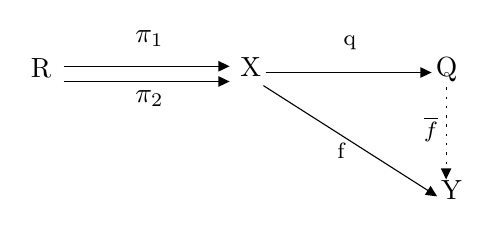
\begin{tikzpicture}[x=0.75pt,y=0.75pt,yscale=-1,xscale=1]
%uncomment if require: \path (0,300); %set diagram left start at 0, and has height of 300

%Straight Lines [id:da7734725100317463]
\draw    (228,147) -- (305,147) ;
\draw [shift={(308,147)}, rotate = 180] [fill={rgb, 255:red, 0; green, 0; blue, 0 }  ][line width=0.08]  [draw opacity=0] (5.36,-2.57) -- (0,0) -- (5.36,2.57) -- cycle    ;
%Straight Lines [id:da007971811961900777]
\draw    (228,154.33) -- (305,154.33) ;
\draw [shift={(308,154.33)}, rotate = 180] [fill={rgb, 255:red, 0; green, 0; blue, 0 }  ][line width=0.08]  [draw opacity=0] (5.36,-2.57) -- (0,0) -- (5.36,2.57) -- cycle    ;
%Straight Lines [id:da3202673895090322]
\draw    (325.33,150) -- (402.33,150) ;
\draw [shift={(405.33,150)}, rotate = 180] [fill={rgb, 255:red, 0; green, 0; blue, 0 }  ][line width=0.08]  [draw opacity=0] (5.36,-2.57) -- (0,0) -- (5.36,2.57) -- cycle    ;
%Straight Lines [id:da7225860259717922]
\draw    (324.33,156.33) -- (405.47,208.05) ;
\draw [shift={(408,209.67)}, rotate = 212.52] [fill={rgb, 255:red, 0; green, 0; blue, 0 }  ][line width=0.08]  [draw opacity=0] (5.36,-2.57) -- (0,0) -- (5.36,2.57) -- cycle    ;
%Straight Lines [id:da21057174956898383]
\draw  [dash pattern={on 0.84pt off 2.51pt}]  (412.33,157.17) -- (412.33,198.5) ;
\draw [shift={(412.33,201.5)}, rotate = 270] [fill={rgb, 255:red, 0; green, 0; blue, 0 }  ][line width=0.08]  [draw opacity=0] (5.36,-2.57) -- (0,0) -- (5.36,2.57) -- cycle    ;

% Text Node
\draw (211,142) node [anchor=north west][inner sep=0.75pt]  [font=\normalsize] [align=left] {R};
% Text Node
\draw (312,141.5) node [anchor=north west][inner sep=0.75pt]   [align=left] {X};
% Text Node
\draw (406.17,141.67) node [anchor=north west][inner sep=0.75pt]   [align=left] {Q};
% Text Node
\draw (408.67,201) node [anchor=north west][inner sep=0.75pt]   [align=left] {Y};
% Text Node
\draw (261.33,128.67) node [anchor=north west][inner sep=0.75pt]   [align=left] {$\displaystyle \pi _{1}$};
% Text Node
\draw (261.33,157.33) node [anchor=north west][inner sep=0.75pt]   [align=left] {$\displaystyle \pi _{2}$};
% Text Node
\draw (361.67,131) node [anchor=north west][inner sep=0.75pt]  [font=\footnotesize] [align=left] {q};
% Text Node
\draw (358.67,183) node [anchor=north west][inner sep=0.75pt]  [font=\footnotesize] [align=left] {f};
% Text Node
\draw (400.5,170.17) node [anchor=north west][inner sep=0.75pt]  [font=\footnotesize] [align=left] {$\overline{f}$};

\end{tikzpicture}

\end{figure}

We can also phrase the universal property of $\kw{Quotient}$ in a type-theoretic way as follows:

\begin{align*}
  & (X/R \rightarrow Y) \simeq \Sigma \ (X \rightarrow Y) \ (\lambda \ f \rightarrow (x \ y : X) \rightarrow \Funapp{R}{x}{y} \rightarrow \Funapp{f}{x} \equiv \Funapp{f}{y}) \\
\end{align*}

This property may be proven within Typer itself. (TODO:\ Actually make this work and direct readers to it).

\subsection{Initial object of quotient set algebras}

Ok maybe let's scratch this, this isn't super interesting.

\chapter{Related works}
\section{HITs}
Higher inductive types (HITs) are a generalisation of inductive types that has been popularized by homotopy type theory\cite{HoTTbook}. Aside from the usual definitions of constructors, HITs allow the definition of path constructors, i.e.\ equalities between terms of the inductive type. Additionally, we are allowed to define paths between paths.
In other words, in a system that supports HITs, we could simply define quotient types as a HIT. For instance, here is how one might do it in Cubical Agda.

\begin{minted}[escapeinside=@@,mathescape=true]{agda}
data _/_ {l l'} (A : Type l) (R : A @$\rightarrow$@ A @$\rightarrow$@ Type l') : Type (l-max l l')
   where
   [_] : (a : A) @$\rightarrow$@ A / R
   eq/ : (a b : A) @$\rightarrow$@ (r : R a b) @$\rightarrow$@ [ a ] @$\equiv$@ [ b ]
   trunc/ : (a b : A / R) @$\rightarrow$@ (p q : a @$\equiv$@ b) @$\rightarrow$@ p @$\equiv$@ q
\end{minted}

In such languages, the elimination of HITs is done in the same manner in which we typically eliminate inductive types, i.e.\ with pattern matching. Path constructors also need to be handled during pattern matching. Explicit side conditions are then added to ensure that the elimination of path constructors is coherent with the elimination of other constructors. To illustrate the above, we describe some HITs that are common in the context of synthetic homotopy theory.

%% FIXME: Why isn't loop of the right colour?
\begin{minted}[escapeinside=@@,mathescape=true]{agda}
data @$S^1$@ : Type where
  base : @$S^1$@
  loop : base @$\equiv$@ base
\end{minted}

%% TODO: I think I need to find a good place to define the word `identify'
The $S^1$ type is a synthetic way of representing a circle (also known as a 1-sphere). A reasonable way of describing a circle would be to say that it consists of a base point and a continuous line that joins the base point to itself. In this HIT, we have the $\id{base}$ as a normal constructor of the type. But more curiously, we also have a path constructor $\id{loop}$ that identifies $\id{base}$ with itself. By visualising the type, we see that it indeed ressembles a circle.

\begin{figure}[H]
  \centering
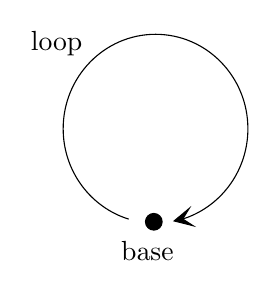
\begin{tikzpicture}[x=0.75pt,y=0.75pt,yscale=-1,xscale=1]
%uncomment if require: \path (0,300); %set diagram left start at 0, and has height of 300

%Shape: Circle [id:dp8752212823145744]
\draw  [fill={rgb, 255:red, 0; green, 0; blue, 0 }  ,fill opacity=1 ] (351,225) .. controls (351,222.79) and (352.79,221) .. (355,221) .. controls (357.21,221) and (359,222.79) .. (359,225) .. controls (359,227.21) and (357.21,229) .. (355,229) .. controls (352.79,229) and (351,227.21) .. (351,225) -- cycle ;
%Shape: Arc [id:dp1917418004201512]
\draw  [draw opacity=0] (342.88,223.71) .. controls (324.62,218.04) and (311.33,200.69) .. (311.33,180.17) .. controls (311.33,155.04) and (331.26,134.67) .. (355.83,134.67) .. controls (380.41,134.67) and (400.33,155.04) .. (400.33,180.17) .. controls (400.33,200.99) and (386.66,218.54) .. (367.99,223.95) -- (355.83,180.17) -- cycle ; \draw   (342.88,223.71) .. controls (324.62,218.04) and (311.33,200.69) .. (311.33,180.17) .. controls (311.33,155.04) and (331.26,134.67) .. (355.83,134.67) .. controls (380.41,134.67) and (400.33,155.04) .. (400.33,180.17) .. controls (400.33,200.99) and (386.66,218.54) .. (367.99,223.95) ;
\draw  [fill={rgb, 255:red, 0; green, 0; blue, 0 }  ,fill opacity=1 ] (373.91,226.89) -- (364.82,224.59) -- (372.03,218.6) -- (368.9,223.67) -- cycle ;

% Text Node
\draw (338,233) node [anchor=north west][inner sep=0.75pt]   [align=left] {base};
% Text Node
\draw (294.5,131.75) node [anchor=north west][inner sep=0.75pt]   [align=left] {loop};


\end{tikzpicture}

\caption{Visualisation of $S^1$}
\end{figure}

To really show how HITs shine, we briefly describe the definition of $\id{double}$ that is a function from $S^1$ to $S^1$ that sends the $\id{loop}$ to the concatenation of two
loops.

\begin{minted}[escapeinside=@@,mathescape=true]{agda}
double : @$S^1$@ @$\rightarrow$@ @$S^1$@
double base = base
double (loop i) = (loop @$\cdot$@ loop) i
\end{minted}

%% TODO: Improve wording here
Pattern matching allows us to `do the job' more cleanly. Aside from that, we get defitional equalities even for path constructors.

TODO:\ Wanted to show an example of HIT-style elimination of a quotient, but I didn't find anything worth showing for now.

\section{QITs and Quotient Haskell}
Points:

Quotient inductive types (QITs) are essentially HITs that are set-truncated. This essentially provides us with the full range of expressiveness of HITs without higher-dimensional paths. In other words, we are not allowed to define paths between paths. Indeed, such paths are not typically used in day-to-day programming tasks.

Compare to Quotient Haskell and cite examples of types that are convenient to define with QITs but are `tedious' to express as our Quotient type.

Requires significantly more work to accomplish, but approximately the same expressive power as quotient types (how true is this!?)? Or do we draw the line at ``in practice, it has comparable expressivity''?
The implementation of QITs would negatively impact the modularity of inductive types.

\section{Quotient by normalisation}
When we take the quotient of a type/set based on an equivalence relation, we are essentially partitioning the elements of the type into their respective equivalence classes. Elements of the same equivalence class are then identified in the resulting quotient type/set.

\begin{figure}[H]
  \centering
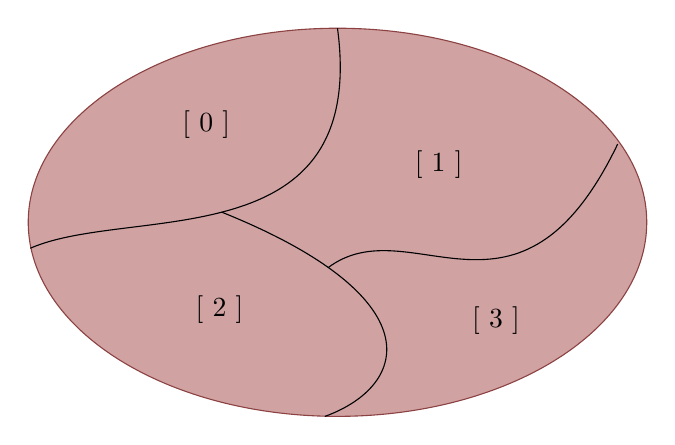
\begin{tikzpicture}[x=0.75pt,y=0.75pt,yscale=-1,xscale=1]
%uncomment if require: \path (0,300); %set diagram left start at 0, and has height of 300

%Shape: Ellipse [id:dp4829810342761349]
\draw  [color={rgb, 255:red, 140; green, 66; blue, 66 }  ,draw opacity=1 ][fill={rgb, 255:red, 208; green, 162; blue, 162 }  ,fill opacity=1 ] (171,152.5) .. controls (171,100.86) and (237.71,59) .. (320,59) .. controls (402.29,59) and (469,100.86) .. (469,152.5) .. controls (469,204.14) and (402.29,246) .. (320,246) .. controls (237.71,246) and (171,204.14) .. (171,152.5) -- cycle ;
%Curve Lines [id:da7772387220169334]
\draw    (172,165) .. controls (220,144) and (335,171) .. (320,59) ;
%Curve Lines [id:da0576638127246778]
\draw    (264.2,147.6) .. controls (366.2,188.6) and (355,231) .. (314,246) ;
%Curve Lines [id:da8789468342677784]
\draw    (315.4,174.4) .. controls (355.4,144.4) and (407.4,213.6) .. (455,114.8) ;

% Text Node
\draw (244,97.6) node [anchor=north west][inner sep=0.75pt]   [align=left] {[ 0 ]};
% Text Node
\draw (356,116.8) node [anchor=north west][inner sep=0.75pt]   [align=left] {[ 1 ]};
% Text Node
\draw (250.4,186.4) node [anchor=north west][inner sep=0.75pt]   [align=left] {[ 2 ]};
% Text Node
\draw (383.6,192) node [anchor=north west][inner sep=0.75pt]   [align=left] {[ 3 ]};


\end{tikzpicture}
\caption{Equivalence classes of $\mathbb{Z}$ under the relation $x \equiv y \ (\kw{mod} \ 4)$}
\end{figure}

An alternative way of defining a quotient on type $\kw{A}$ under a relation $\kw{R}$ is to construct a function $\oftype{\id{nf}}{A \rightarrow A}$ such that $\Funapp{\id{nf}}{\id{a}}$ is the canonical representative of the equivalence class that $\id{a}$ belongs to. This approach is comparable to \cite{courtieu-normalizedtypes}. In other words, for $\oftype{x, y}{A}$, $\Funapp{\kw{Eq}}{(\Funapp{\kw{Quotient\_in}}{\id{x}})}{(\Funapp{\kw{Quotient\_in}}{\id{y}})} \iff \Funapp{\kw{Eq}}{(\Funapp{\id{nf}}{\id{x}})}{(\Funapp{\id{nf}}{\id{y}})}$. To represent this in our system, we can simply treat this as a quotient under the relation $\Funapp{\id{R}}{\id{x}}{\id{y}} = \Funapp{\kw{Eq}}{(\Funapp{\id{nf}}{\id{x}})}{(\Funapp{\id{nf}}{\id{y}})}$.

To simplify the utilisation of this class of quotients in Typer programs, we define the following helper functions:

\begin{minted}[escapeinside=@@,mathescape=true]{haskell}
Qnorm : (A : Type) @$\rightarrow$@ (nf : A @$\rightarrow$@ A) @$\rightarrow$@ Type
Qnorm A nf = Quotient A (@$\lambda$@ x y @$\rightarrow$@ Eq (nf x) (nf y))

Qnorm_in : ?A @$\rightarrow$@ Qnorm ?A ?nf;
Qnorm_in a = Quotient_in a;

Qnorm_elim : Qnorm ?A ?nf @$\rightarrow$@ (?A @$\rightarrow$@ ?B) @$\rightarrow$@ ?B
Qnorm_elim q f = Quotient_rec (f @$\circ$@ nf)
                              (p := @$\lambda$@ x y r @$\rightarrow$@ Eq_cong f r)
                              q

Qnorm_eq : (a a' : ?A) @$\rightarrow$@ Eq (nf a) (nf a') @$\rightarrow$@ Eq (Qnorm_in a) (Qnorm_in a')
Qnorm_eq a a' eq = Quotient_eq (a := a') (a' = a') eq
\end{minted}

We could have alternatively introduced quotients to Typer by implementing the above as a built-in construct instead of what we have implemented currently. However, as we have demonstrated above, this flavour of quotients is a strict subset of our implementation. Implying that this is less expressive and flexible compared to our implementation. Indeed, it is not always possible to define a normalisation function for a certain equivalence relation (TODO:\ Construct a convincing example). However, this approach also has its advantages, notably in Courtieu's system \cite{courtieu-normalizedtypes}, $\Funapp{\kw{Eq}}{(\Funapp{\id{nf}}{\id{x}})}{(\Funapp{\id{nf}}{\id{y}})} \Rightarrow \Funapp{\kw{Eq}}{(\Funapp{\kw{Quotient\_in}}{\id{x}})}{(\Funapp{\kw{Quotient\_in}}{\id{y}})}$ actually deals with definitional equivalences instead of propositional equivalences as is done with $Qnorm\_eq$.

Quotients based on normalisation may actually be represented in Typer without extending the language. Indeed, this can be done in any language that supports coproducts, as is suggested in \cite{HoTTbook}. Similarly, Courtieu's implementation may also be translated to the Calculus of Inductive Constructions \cite{werner-cic}. We now describe the aforementioned construction in Typer, and then provide a proof that it fulfils the universal property of a quotient.

We define a dependent pair as follows (this is why we require coproducts):

\begin{minted}[escapeinside=@@,mathescape=true]{haskell}
type Sigma (A : Type) (B : A @$\rightarrow$@ Type)
  | sigma (fst : A) (snd : B fst);
\end{minted}

Now, we can define the type $\kw{Qnorm}$ for some type $\id{A}$ and normalisation function $\oftype{r}{A \rightarrow A}$ as a dependent pair that contains some term of type $\id{A}$ and a proof that it has been normalised. This of course necessitates the idempotency of the normalisation function.

\begin{minted}[escapeinside=@@,mathescape=true]{haskell}
Qnorm : (A : Type) @$\rightarrow$@ isSet A @$\rightarrow$@ (r : A @$\rightarrow$@ A)
        @$\rightarrow$@ (i : (x : A) @$\rightarrow$@ Eq (r (r x)) (r x)) @$\rightarrow$@ Type
Qnorm A p r i = Sigma A (@$\lambda$@ (x : A) @$\rightarrow$@ Eq (r x) x)
\end{minted}

The injection into $\kw{Qnorm}$ is simply the construction of a dependent pair containing a term that has been normalised and a proof of its normalisation. This is in contrast to the construction that was described previously with $\kw{Quotient}$ which applied the normalisation upon the elimination of a quotient, whereas here, normalisation immediately occurs upon the construction of a term of type $\kw{Qnorm}$.

We can prove that the equality of $\kw{Qnorm}$ terms is characterised by the equality between the normalised forms of the underlying terms. As usual, we require $\Funapp{\kw{isSet}}{\id{A}}$ to prove this equality. A simple invocation of the ${\Sigma}{\equiv}$\_prop lemma completes the proof.


\begin{minted}[escapeinside=@@,mathescape=true]{haskell}
Qnorm_eq : (A : Type) @$\Rrightarrow$@ (x y : A) @$\Rightarrow$@ (p : HoTT_isSet A)
           @$\Rightarrow$@ (r : A @$\rightarrow$@ A) @$\Rightarrow$@ (i : (x : A) @$\rightarrow$@ Eq (r (r x)) (r x))
           @$\Rightarrow$@ Eq (r x) (r y) @$\rightarrow$@ Eq (Qnorm_in (p := p) (r := r) (i := i) x)
                                   (Qnorm_in (p := p) (r := r) (i := i) y)
Qnorm_eq = @$\lambda$@ A @$\Rrightarrow$@ @$\lambda$@ x y p r i @$\Rightarrow$@ @$\lambda$@ rx@$\equiv$@ry @$\rightarrow$@
  @${\Sigma}{\equiv}$@_prop (B := @$\lambda$@ x @$\rightarrow$@ Eq (r x) x)
           (@$\lambda$@ x @$\rightarrow$@ p (r x) x)
           (sigma (B := @$\lambda$@ x @$\rightarrow$@ Eq (r x) x) (r x) (i x))
           (sigma (B := @$\lambda$@ x @$\rightarrow$@ Eq (r x) x) (r y) (i y))
           rx@$\equiv$@ry
\end{minted}

We can easily prove the reverse of this too, i.e. if we have that $\Funapp{\kw{Eq}}{(\Funapp{\kw{Qnorm\_in}}{x})}{(\Funapp{\kw{Qnorm\_in}}{y})}$, then $\Funapp{\kw{Eq}}{(\Funapp{r}{x})}{(\Funapp{r}{y})}$ is immediate by taking the first projection of the pairs.

Finally, we can also show that $\kw{Qnorm}$ fulfils the universal property of a quotient. In other words, we want show the following equivalence:

\begin{align*}
  & (\Funapp{\kw{Qnorm}}{A}{p}{r}{i} \rightarrow B) \simeq \Sigma \ (A \rightarrow B) \ (\lambda g \rightarrow (x \ y : A) \rightarrow \Funapp{r}{x} \equiv \Funapp{r}{y} \rightarrow \Funapp{g}{x} \equiv \Funapp{g}{y})
\end{align*}

The proof itself is not very interesting, hence we do not describe it here. (TODO:\ Link to proof). We note however that the reverse direction of this equivalence gives us a means of eliminating $\kw{Qnorm}$, as was the case for $\kw{Quotient}$.

TODO: Mention how we could also have an NF of type $A \rightarrow B$, i.e. doesn't have to be the same type as the base type, but obviously this doesn't work with this precise construction.


%%--------------%
%%     index    %
%%--------------%

%% S'il y a lieu, décommenter la ligne pour mettre votre index

%%\printindex

%%------------------------------------------------- %
%%         références --- bibliographie             %
%%------------------------------------------------- %

\def\bibname{References}
\bibliography{main}
\bibliographystyle{ieeetr}



%%------------------------------------------------- %
%%                  Annexe A                        %
%%------------------------------------------------- %

\anglais
\appendix

\chapter{Equational Reasoning}\label{section:eqreasoning}
Equational reasoning provides us with a neat way of expressing proofs in Typer. With the help of some syntactic sugar, this allows us to build chains of equality proofs by using the transitivity property of equality as shown in Section~\ref{subsection:eqtransitivity}. This is something that is implemented in the libraries of most proof assistants, such as Agda, Lean, and Lean. This allows lengthy proofs to remain readable as intermediate steps are documented and are clearly seen.

First, we introduce a helper function that simply invokes the transitivity property of equality proofs. This function carries out a single step of equational reasoning.

\begin{minted}[escapeinside=@@,mathescape=true]{haskell}
step-@$\equiv$@ : (x : ?A) @$\rightarrow$@ (y : ?A) @$\rightarrow$@ (z : ?A) @$\rightarrow$@ Eq x y @$\rightarrow$@ Eq y z @$\rightarrow$@ Eq x z
step-@$\equiv$@ _ p q = Eq_trans p q
\end{minted}

Next, we require a second function to conclude a chain of equational reasoning.

\begin{minted}[escapeinside=@@,mathescape=true]{haskell}
qed : (x : ?A) @$\rightarrow$@ Eq x x
qed x = Eq_refl
\end{minted}

To make it all come together, we wrap the above functions with some syntaxic sugar.

\begin{minted}[escapeinside=@@,mathescape=true]{haskell}
_==<_>==_ = step-@$\equiv$@
_@$\qed$@ = qed
\end{minted}

%% TODO:\ Make \_$\qed$ look nicer
\verb|_==<_>==_| can be seen as a mixfix operator, whereas \_$\qed$ is a postfix operator.

When we write the following

\begin{lstlisting}
  x
  ==< p >==
  y
  ==< ... >==
  .
  .
  .
  ==< ... >==
  z $\qed$
\end{lstlisting}

We require that $\id{p}$ be a proof of equality between $\id{x}$ and $\id{y}$, and this can be chained \latinphrase{ad infinitum}. The expression in its entirety is a proof of equality between $\id{x}$ and $\id{z}$. The usage of this is best illustrated via a simple example:

\begin{minted}[escapeinside=@@,mathescape=true]{haskell}
example : (x : ?A) @$\rightarrow$@ (y : ?A) @$\rightarrow$@ (z : ?A) @$\rightarrow$@ (w : ?A)
          @$\rightarrow$@ (p : Eq x y) @$\rightarrow$@ (q : Eq y z) @$\rightarrow$@ (r : Eq z w) @$\rightarrow$@ Eq x w
example x y z w p q r =
  x ==< p >==
  y ==< q >==
  z ==< r >==
  w @$\qed$@
\end{minted}

For a more involved example, we rewrite the proof of \verb|Integer_*DistR+| that was shown in Section~\ref{subsection:int-theorems} by using equational reasoning.

\begin{minted}[escapeinside=@@,mathescape=true]{haskell}
Integer_*DistR+ : (x : Integer) @$\rightarrow$@ (y : Integer) @$\rightarrow$@ (z : Integer)
                  @$\rightarrow$@ Eq (Integer_* x (Integer_+ y z))
                        (Integer_+ (Integer_* x y) (Integer_* x z))
Integer_*DistR+ x y z =
  Integer_* x (Integer_+ y z)
  ==< Integer_*-comm x (Integer_+ y z) >==
  Integer_* (Integer_+ y z) x
  ==< Integer_*DistL+ y z x >==
  Integer_+ (Integer_* y x) (Integer_* z x)
  ==< Eq_cong (flip Integer_+ (Integer_* z x)) (Integer_*-comm y x) >==
  Integer_+ (Integer_* x y) (Integer_* z x)
  ==< Eq_cong (Integer_+ (Integer_* x y)) (Integer_*-comm z x) >==
  Integer_+ (Integer_* x y) (Integer_* x z) @$\qed$@
\end{minted}

TODO:\ Consider adding a discussion on additional macros and tactics that could be added to ease the development of such proofs, e.g.\ it would be nice to have rewrite tactics that Lean has to avoid having to invoke Eq\_cong that often

\chapter{Other proofs}\label{app:other-proofs}

\section{Commutativity of addition of natural numbers}

We first define the type of natural numbers along with the addition operation
the usual way.

\begin{minted}[escapeinside=@@,mathescape=true]{haskell}
Nat : Type

type Nat
  | zero
  | succ Nat

_+_ : Nat @$\rightarrow$@ Nat @$\rightarrow$@ Nat
_+_ x y = case x
  | zero @$\Rightarrow$@ y
  | succ m @$\Rightarrow$@ succ (m + y)
\end{minted}

We then define two lemmas that we ultimately use to prove the commutativity of
addition.

\begin{minted}[escapeinside=@@,mathescape=true]{haskell}
Nat+_zero : (m : Nat) @$\rightarrow$@ Eq (m + zero) m
Nat+_zero m =
  case m return Eq (m + zero) m
         | zero @$\Rightarrow$@ Eq_refl
         | succ n @$\Rightarrow$@ Eq_cong succ (Nat+_zero n)

Nat+_succ : (m : Nat) @$\rightarrow$@ (n : Nat) @$\rightarrow$@ Eq (m + succ n) (succ (m + n))
Nat+_succ m n =
  case m return Eq (m + succ n) (succ (m + n))
         | zero @$\Rightarrow$@ Eq_refl
         | succ m' @$\Rightarrow$@ Eq_cong succ (Nat+_succ m' n)

Nat+_comm : (m : Nat) @$\rightarrow$@ (n : Nat) @$\rightarrow$@ Eq (m + n) (n + m)
Nat+_comm m n =
  case n return Eq (m + n) (n + m)
         | zero @$\Rightarrow$@ Nat+_zero m
         | succ n' @$\Rightarrow$@ Eq_trans (Nat+_succ m n')
                               (Eq_cong succ (Nat+_comm m n'))
\end{minted}

\chapter{Les différentes parties et leur ordre d'apparition}

%% TODO: Don't forget to ultimately remove this!

J'ajoute ici les différentes parties d'un mémoire ou d'une thèse ainsi
que leur ordre d'apparition tel que décrit dans le guide de
présentation des mémoires et des thèses de la Faculté des études
supérieures.  Pour plus d'information, consultez le guide sur le site
web de la facutlé (www.fes.umontreal.ca).

\newcount\colnum
\colnum=1
\def\i{\number\colnum. \global\advance\colnum by 1\ignorespaces}
\begin{table}[p]
  \begin{center}
    \begin{tabular}{|l|l|r|}\hline
       \noindent\hfil
         \textbf{\strut Ordre des éléments constitutifs du mémoire ou de la thèse}
         \hfil\span\omit\span\omit\\\hline % \span\omit pour couvrir plus d'une
                                           % case sans utiliser le package multirow ou autre
      \i &  La page de titre & obligatoire\\\hline
      \i &  La page d'identification des membres du jury & obligatoire\\\hline
      \i &  Le résumé en français et les mots clés français\kern3em& obligatoires\\\hline
      \i &  Le résumé en anglais et les mots clés anglais & obligatoires\\\hline
      \i &  Le résumé dans une autre langue que l'anglais & obligatoire \\
         &  ou le français (si le document est écrit dans &\\
         &  une autre langue que l'anglais ou le français)&\\\hline
      \i &  Le résumé de vulgarisation& facultatif\\\hline
      \i &  La table des matières, la liste des tableaux,& obligatoires\\
         &   la liste des figures ou autre &\\\hline
      \i &  La liste des sigles et des abréviations& obligatoire\\\hline
      \i &  La dédicace& facultative\\\hline
      \i &  Les remerciements & facultatifs\\\hline
      \i &  L'avant-propos & facultatif\\\hline
      \i &  Le corps de l'ouvrage& obligatoire\\\hline
      \i &  Les index& facultatif\\\hline
      \i &  Les références bibliographiques & obligatoires\\\hline
      \i &  Les annexes & facultatifs\\\hline
      \i &  Les documents spéciaux & facultatifs\\\hline
    \end{tabular}
  \end{center}
\end{table}

\end{document}

\endinput
%%
%% End of file `gabaritmem.tex'.
